\chapter[NFSWEs的原始能量和质量守恒方法]{NFSWEs的原始能量和质量守恒方法}
据了解, 目前针对 NFSWEs 的数值方法只能保证修正后的能量和(或)质量守恒.
注意到最近提出的分区平均向量场系列方法不仅可以保持原始能量,还有可能保持更多的守恒性质,并且已被用于构造哈密顿常微分方程的守恒数值方案\cite{caiPartitionedAveragedVector2018}.
本章通过升级版的平均向量场方法为NFSWEs构建了能同时保持原始能量和质量的数值方法.
\section{NFSWEs的哈密顿格式}\label{Section_PAVF: 2_1}

哈密顿结构是构建PAVF系列格式的前提.然而,目前没有研究人员考虑过具有周期性边界条件的NFSWEs \eqref{eq_SAVRRK:1}-\eqref{eq_SAVRRK:3} 的哈密顿结构.
基于此, 本小节推导了 NFSWEs 的哈密顿结构.

设
\begin{align}
u = p+\mathrm{i}q, \quad u_t = \varphi+ \mathrm{i}\psi,
\end{align}
其中$p, q,\varphi,\psi$均为实值函数.那么,NFSWEs \eqref{eq_SAVRRK:1}-\eqref{eq_SAVRRK:3} 可以重写为
\begin{align}\label{eq_PAVF:28}
\varphi_{t}+\mathrm{i}\psi_{t}+\left( -\Delta \right) ^{\frac{\alpha }{2}}p+\mathrm{i}\left( -\Delta \right) ^{\frac{\alpha }{2}}q+\mathrm{i}\kappa \varphi-\kappa \psi+\beta \left( p^{2}+q^{2}\right) \left( p+\mathrm{i} q\right) =0.
\end{align}
分离实部和虚部,得到
\begin{align}
&\varphi_{t}+\left( -\Delta \right) ^{\frac{\alpha }{2}}p-\kappa \psi+\beta \left( p^{2}+q^{2}\right)p=0,\nonumber\\
&\psi_{t}+\left( -\Delta \right) ^{\frac{\alpha }{2}}q+\kappa \varphi+\beta \left( p^{2}+q^{2}\right)q=0.\label{eq_PAVF:29}
\end{align}
即,NFSWEs \eqref{eq_SAVRRK:1}-\eqref{eq_SAVRRK:3} 可以重写为一个等价的耦合系统
\begin{align}
&\varphi_{t}=-\left( -\Delta \right) ^{\frac{\alpha }{2}}p+\kappa \psi-\beta \left( p^{2}+q^{2}\right)p\label{eq_PAVF:30},\\
&\psi_{t}=-\left( -\Delta \right) ^{\frac{\alpha }{2}}q-\kappa \varphi-\beta \left( p^{2}+q^{2}\right)q\label{eq_PAVF:31},\\
&p_t=\varphi, \label{eq_PAVF:32}\\
&q_t=\psi, \label{eq_PAVF:33}
\end{align}
其中$p, q,\varphi,\psi$满足周期性边界条件.

为了得到NFSWEs \eqref{eq_SAVRRK:1}-\eqref{eq_SAVRRK:3} 的哈密顿形式,引入以下两个重要引理.
\begin{lemma}\label{lem_PAVF:1}
	\cite{fuStructurepreservingAlgorithmsTwodimensional2020} 
	 给定 $1<\alpha \leq 2$,那么对于任何实周期函数 $p, q \in L^{2}(\Omega)$,有
	\begin{align}\label{eq_PAVF:22}
	\int_{\Omega}(-\Delta)^{\frac{\alpha}{2}} p q d \boldsymbol{x}=\int_{\Omega}(-\Delta)^{\frac{\alpha}{4}} p(-\Delta)^{\frac{\alpha}{4}} q d \boldsymbol{x}=\int_{\Omega} p(-\Delta)^{\frac{\alpha}{2}} q d \boldsymbol{x}.
	\end{align}
	\end{lemma}

\begin{proof}
	根据 Plancherel 定理,有
\begin{equation}
\begin{aligned}
\int_{\Omega}(-\Delta)^{\frac{\alpha}{2}} p q d \boldsymbol{x} &=(2 L)^{2} \sum_{l_{1} \in \mathbb{Z}} \sum_{l_{2} \in \mathbb{Z}}\left|v_{l_{1}}^{2}+v_{l_{2}}^{2}\right|^{\frac{\alpha}{2}} \hat{p}_{l_{1}, l_{2}} \hat{q}_{l_{1}, l_{2}} \\
&=(2 L)^{2} \sum_{l_{1} \in \mathbb{Z}} \sum_{l_{2} \in \mathbb{Z}}\left|v_{l_{1}}^{2}+v_{l_{2}}^{2}\right|^{\frac{\alpha}{4}} \hat{p}_{l_{1}, l_{2}}\left|v_{l_{1}}^{2}+v_{l_{2}}^{2}\right|^{\frac{\alpha}{4}} \hat{q}_{l_{1}, l_{2}} \\
&=(2 L)^{2} \sum_{l_{1} \in \mathbb{Z}} \sum_{l_{2} \in \mathbb{Z}} \hat{p}_{l_{1}, l_{2}}\left|v_{l_{1}}^{2}+v_{l_{2}}^{2}\right|^{\frac{\alpha}{2}} \hat{q}_{l_{1}, l_{2}} .
\end{aligned}
\label{eq_23}\end{equation}
于是
\begin{equation}
\int_{\Omega}(-\Delta)^{\frac{\alpha}{2}} p q d \boldsymbol{x}=\int_{\Omega}(-\Delta)^{\frac{\alpha}{4}} p(-\Delta)^{\frac{\alpha}{4}} q d x=\int_{\Omega} p(-\Delta)^{\frac{\alpha}{2}} q d \boldsymbol{x}
\label{eq_24}\end{equation}
证毕.
\end{proof}


\begin{lemma}\label{lem_PAVF:2}
	\cite{wangStructurepreservingNumericalMethods2018} 
	 对于形如
	\begin{align}\label{eq_PAVF:25}
	F[g]=\int_{\Omega} f\left(g(\boldsymbol{x}),(-\Delta)^{\frac{\alpha}{4}} g(\boldsymbol{x})\right) d \boldsymbol{x},
	\end{align}
	的泛函 $F[g]$, $f$ 是 $\Omega$ 上的光滑函数,其变分导数如下
	\begin{align}\label{eq_PAVF:26}
	\frac{\delta F}{\delta g}=\frac{\partial f}{\partial g}+(-\Delta)^{\frac{\alpha}{4}} \frac{\partial f}{\partial\left((-\Delta)^{\frac{\alpha}{4}} g\right)} .
	\end{align}
	\end{lemma}

\begin{proof}
	令 $\phi(\boldsymbol{x})$ 为具有周期性边界条件的任意函数.由于分数阶拉普拉斯算子是线性算子,根据变分导数的定义,有
\begin{equation}
\begin{aligned}
\int_{\Omega} \frac{\delta F}{\delta g} \phi(\boldsymbol{x}) d \boldsymbol{x} &=\left[\frac{d}{d \mu} \int_{\Omega} f\left(g+\mu \phi,(-\Delta)^{\frac{\alpha}{4}} g+\mu(-\Delta)^{\frac{\alpha}{4}} \phi\right) d \boldsymbol{x}\right]_{\mu=0} \\
&=\int_{\Omega}\left(\frac{\partial f}{\partial g} \phi+\frac{\partial f}{\partial\left((-\Delta)^{\frac{\alpha}{4}} g\right)}(-\Delta)^{\frac{\alpha}{4}} \phi\right) d \boldsymbol{x}\\
&=\int_{\Omega}\left(\frac{\partial f}{\partial g} \phi+\left((-\Delta)^{\frac{\alpha}{4}} \frac{\partial f}{\partial\left((-\Delta)^{\frac{\alpha}{4}} g\right)}\right) \phi\right) d \boldsymbol{x} \\
&=\int_{\Omega}\left(\frac{\partial f}{\partial g}+(-\Delta)^{\frac{\alpha}{4}} \frac{\partial f}{\partial\left((-\Delta)^{\frac{\alpha}{4}} g\right)}\right) \phi d \boldsymbol{x},
\end{aligned}
\label{eq_27}\end{equation}
其中使用了 式\eqref{eq_PAVF:22}.基于 $\phi(\boldsymbol{x})$ 的任意性,通过变分法基本引理,可以得到 式\eqref{eq_PAVF:26}.
\end{proof}

基于上述引理,可以得到以下结果.

\begin{theorem}	\label{thm_PAVF:2_1}
设
\begin{align}
&\mathcal{G}=\kappa\int_{\Omega}(p^2+q^2) d \boldsymbol{x}+2\operatorname{Im}(\int_{\Omega}(\varphi+\mathrm{i}\psi)(p-\mathrm{i}q)d \boldsymbol{x}),\label{eq_PAVF:34} \\
&\mathcal{H}=\frac{1}{2}\int_{\Omega}\left((\varphi^2+\psi^2)+\left((-\Delta)^{\frac{\alpha}{4}} p\right)^{2}+\left((-\Delta)^{\frac{\alpha}{4}} q\right)^{2}+\frac{\beta}{2}(p^2+q^2)^{2}\right) d \boldsymbol{x}.\label{eq_PAVF:35}
\end{align}
那么等价系统 \eqref{eq_PAVF:30}-\eqref{eq_PAVF:33} 具有以下两个守恒定律:
\begin{align}
\frac{d}{d t} \mathcal{G}=0, \quad \frac{d}{d t} \mathcal{H}=0.
\end{align}
\end{theorem}

\begin{proof}
将式 \eqref{eq_PAVF:30} 和 式\eqref{eq_PAVF:31} 分别与 $\varphi$ 和 $\psi$ 做内积,可以立即得到第一个守恒定律.
注意到引理 \ref{lem_PAVF:1},并将方程 \eqref{eq_PAVF:30}-\eqref{eq_PAVF:33} 与 $\varphi_{t}, \psi_{t}, p_{t},-q_{t}$ 分别做内积,可以推导出第二个守恒定律.
\end{proof}

\begin{theorem}\label{thm_PAVF:2}
	NFSWEs \eqref{eq_SAVRRK:1}-\eqref{eq_SAVRRK:3} 可以被重构为以下哈密顿系统
\begin{equation}\label{eq_PAVF:37}
	\left(\begin{array}{l}
		\varphi_{t} \\
		\psi_{t} \\
		p_{t} \\
		q_{t}
		\end{array}\right)=J\left(\begin{array}{l}
		\delta \mathcal{H} / \delta \varphi \\
		\delta \mathcal{H} / \delta \psi \\
		\delta \mathcal{H} / \delta p \\
		\delta \mathcal{H} / \delta q
		\end{array}\right),
\end{equation}
其中能量泛函 $\mathcal{H}$ 定义如 式\eqref{eq_PAVF:35}, 哈密顿算符
\begin{equation}\label{eq_PAVF:37b}
J=\left(\begin{array}{cccc}
		0 & \kappa & -1 & 0 \\
		-\kappa & 0 & 0 & -1 \\
		1 & 0 & 0 & 0 \\
		0 & 1 & 0 & 0
		\end{array}\right).
\end{equation}
\end{theorem}

\begin{proof}
注意到
\begin{align}\label{eq_PAVF:12071}
(-\Delta)^{\frac{\alpha}{4}}((-\Delta)^{\frac{\alpha}{4}}  u(\boldsymbol{x},t))&=\mathcal{F}^{-1}\left[|\boldsymbol{\sigma}|^{\frac{\alpha}{2}} \mathcal{F}(\mathcal{F}^{-1}\left[|\boldsymbol{\sigma}|^{\frac{\alpha}{2}} \mathcal{F}(u(\boldsymbol{\sigma},t))\right])\right]\nonumber\\
&=\mathcal{F}^{-1}\left[|\boldsymbol{\sigma}|^{\frac{\alpha}{2}} |\boldsymbol{\sigma}|^{\frac{\alpha}{2}} \mathcal{F}(u(\boldsymbol{\sigma},t))\right]\nonumber\\
&=\mathcal{F}^{-1}\left[|\boldsymbol{\sigma}|^{\alpha} \mathcal{F}(u(\boldsymbol{\sigma},t))\right]\nonumber\\
&=(-\Delta)^{\frac{\alpha}{2}} u(\boldsymbol{x},t),
\end{align}
并应用引理 \ref{lem_PAVF:2} 中的分数阶变分原理,得到
\begin{align}
\frac{\delta \mathcal{H}}{\delta p} &=\frac{1}{2}\left(2(-\Delta)^{\frac{\alpha}{2}} p+2 \cdot \frac{\beta}{2}\left(p^{2}+q^{2}\right) \cdot 2 p\right)=(-\Delta)^{\frac{\alpha}{2}}p+\beta\left(p^{2}+q^{2}\right) p,\label{eq_PAVF:38a}\\
\frac{\delta \mathcal{H}}{\delta q} &=\frac{1}{2}\left(2(-\Delta)^{\frac{\alpha}{2}} q+2 \cdot \frac{\beta}{2}\left(p^{2}+q^{2}\right) \cdot 2 q\right)=(-\Delta)^{\frac{\alpha}{2}}q+\beta\left(p^{2}+q^{2}\right) q,\label{eq_PAVF:38b}\\
\frac{\delta \mathcal{H}}{\delta \varphi} &=\varphi,\label{eq_PAVF:38c}\\
\frac{\delta \mathcal{H}}{\delta \psi} &=\psi.\label{eq_PAVF:38}
\end{align}
结合 NFSWEs \eqref{eq_SAVRRK:1}-\eqref{eq_SAVRRK:3} 的等价形式 \eqref{eq_PAVF:30}-\eqref{eq_PAVF:33},可得到
\begin{equation}\label{eq_PAVF:39}
\left(\begin{array}{l}
		\varphi_{t} \\
		\psi_{t} \\
		p_{t} \\
		q_{t}
\end{array}\right)
=\left(\begin{array}{cccc}
			0 & \kappa & -1 & 0 \\
			-\kappa & 0 & 0 & -1 \\
			1 & 0 & 0 & 0 \\
			0 & 1 & 0 & 0
\end{array}\right)
\left(\begin{array}{l}
		\delta \mathcal{H} / \delta \varphi \\
		\delta \mathcal{H} / \delta \psi \\
		\delta \mathcal{H} / \delta p \\
		\delta \mathcal{H} / \delta q
\end{array}\right).
\end{equation}
证毕.
\end{proof}

\section{傅里叶拟谱离散格式}\label{Section_PAVF: 2_2}

鉴于周期性边界条件,选择傅里叶拟谱法离散等价系统 \eqref{eq_PAVF:30}-\eqref{eq_PAVF:33},
得到如下的空间半离散系统
\begin{align}
&\varPhi_{t}=D^{\alpha}P+\kappa \Psi-\beta \left( P^{2}+Q^{2}\right)\cdot P,\label{eq_PAVF:56}\\
&\Psi_{t}=D^{\alpha}Q-\kappa \varPhi-\beta \left( P^{2}+Q^{2}\right)\cdot Q,\label{eq_PAVF:57}\\
&P_t=\varPhi,\label{eq_PAVF:58}\\
&Q_t=\Psi,\label{eq_PAVF:59}
\end{align}
其中$P^{2}=P \cdot P$.

简洁起见,定义向量
\begin{align}\label{eq_PAVF:60a}
Y=\left(\varPhi^{T}, \Psi^{T}, P^{T}, Q^{T}\right),
\end{align}
则上述半离散系统可重写为如下哈密顿形式
\begin{align}\label{eq_PAVF:60}
\frac{d Y}{d t}=f(Y)=S \nabla H(Y),
\end{align}
哈密顿能量定义如下
\begin{align}\label{eq_PAVF:61}
	H(Y)=\frac{1}{2}\left((\varPhi^{T}\varPhi+\Psi^{T}\Psi){-P^{T} D^{\alpha} P-Q^{T} D^{\alpha} Q}+\frac{\beta}{2}(P^2+Q^2)^{T}(P^2+Q^2)\right),
\end{align}
其中$S$是具有以下形式的反对称矩阵
\begin{align}\label{eq_PAVF:62}
S=\left(\begin{array}{cccc}
0 & \kappa I & -I & 0 \\
-\kappa I & 0 & 0 & -I \\
I & 0 & 0 & 0 \\
0 & I & 0 & 0
\end{array}\right).
\end{align}
此外,定义质量
\begin{align}\label{eq_PAVF:63}
G(Y)=\kappa\|P\|^{2}+\kappa\|Q\|^{2} +2\Psi^{T}P-2\varPhi^{T}Q.
\end{align}
% 接下来有以下定理.

\begin{theorem}	\label{thm_PAVF:3}
	半离散系统 \eqref{eq_PAVF:56}-\eqref{eq_PAVF:59} 具有质量和能量守恒定律
\begin{align}
\frac{d G(Y)}{d t}=0,~\frac{d H(Y)}{d t}=0.
\end{align}
\end{theorem}

\begin{proof}
	根据式 \eqref{eq_PAVF:63},可以推导出
	\begin{align}\label{eq_PAVF:64}
		\frac{d G(Y)}{d t}=&~2 h_{x} h_{y}\left(\kappa P^{T}P_t+\kappa Q^{T}Q_t+\Psi^{T}_t P+\Psi^{T}P_{t}-\varPhi^{T}_t Q-\varPhi^{T}Q_{t}\right)\nonumber\\
		=&~2 h_{x} h_{y}\left(\kappa P^{T}\varPhi+\kappa Q^{T}\Psi {+ P^{T}D^{\alpha}Q}-\kappa P^{T}\varPhi-\beta P^{T}\left( P^{2}+Q^{2}\right)\cdot Q\right.\nonumber\\
		&~\left.+\Psi^{T}\varPhi{-Q^{T}D^{\alpha}P}-\kappa Q^{T}\Psi+\beta Q^{T}\left( P^{2}+Q^{2}\right)\cdot P-\varPhi^{T}\Psi\right)\nonumber\\
		=&~0.
		\end{align}
		基于矩阵 $S$ 的反对称性质,结合式 \eqref{eq_PAVF:60},有
		\begin{equation}\label{eq_PAVF:65}
		\frac{d H(Y)}{d t}=\nabla H(Y)^{T} f(Y)=\nabla H(Y)^{T} S \nabla H(Y)=0 .
		\end{equation}
		证毕.
		\end{proof}

\section{PAVF-P 方法}\label{Section_PAVF: 3}
对于NFSWEs\eqref{eq_SAVRRK:1}-\eqref{eq_SAVRRK:3},如表\ref{tab:NFSWEs}所示存在许多保结构的方法,但其中大多数只保持修正后的能量或质量.
本小节基于等价哈密顿系统\eqref{eq_PAVF:60},通过PAVF-P方法\cite{caiPartitionedAveragedVector2018}为NFSWEs构建了能够同时保持原始能量和质量的数值格式.

\subsection{PAVF-P 格式}
对哈密顿系统\eqref{eq_PAVF:60}应用PAVF方法,得到NFSWEs \eqref{eq_SAVRRK:1}-\eqref{eq_SAVRRK:3} 的全离散格式如下
\begin{align}
\delta_{t} \varPhi^{m}=&\int_{0}^{1}\kappa H_{\Psi}\left(\varPhi^{m+1}, \varepsilon \Psi^{m+1}+(1-\varepsilon) \Psi^{m}, P^{m}, Q^{m}\right)d \varepsilon\nonumber\\
&-\int_{0}^{1}H_{P}\left(\varPhi^{m+1}, \Psi^{m+1}, \varepsilon P^{m+1}+(1-\varepsilon) P^{m}, Q^{m}\right)d \varepsilon,\label{eq_PAVF:70}\\
\delta_{t} \Psi^{m}=&-\int_{0}^{1}\kappa H_{\varPhi}\left(\varepsilon \varPhi^{m+1}+(1-\varepsilon) \varPhi^{m}, \Psi^{m}, P^{m}, Q^{m}\right)d \varepsilon\nonumber\\
&+\int_{0}^{1}H_{Q}\left(\varPhi^{m+1}, \Psi^{m+1}, P^{m+1}, \varepsilon Q^{m+1}+(1-\varepsilon) Q^{m}\right)d\varepsilon,\label{eq_PAVF:71}\\
\delta_{t} P^{m}=&\int_{0}^{1}H_{\varPhi}\left(\varepsilon \varPhi^{m+1}+(1-\varepsilon) \varPhi^{m}, \Psi^{m}, P^{m}, Q^{m}\right) d \varepsilon,\label{eq_PAVF:72}\\
\delta_{t} Q^{m}=&\int_{0}^{1}H_{\Psi}\left(\varPhi^{m+1}, \varepsilon \Psi^{m+1}+(1-\varepsilon) \Psi^{m}, P^{m}, Q^{m}\right) d \varepsilon.\label{eq_PAVF:73}
\end{align}
上述数值格式可以进一步整合为如下傅里叶拟谱 PAVF(FPAVF)格式
\begin{align}
\delta_{t} \varPhi^{m}=&~\kappa \Psi^{m+\frac{1}{2}}{+D^{\alpha} P^{m+\frac{1}{2}}}-\frac{\beta}{4}\left( (P^{m+1})^3+ (P^{m})^{2}\cdot P^{m+1}+(P^{m+1})^{2}\cdot P^{m}\right.\nonumber\\
	&+\left. (P^{m})^{3}+2 P^{m+1}\cdot (Q^{m})^{2}+2 P^{m}\cdot (Q^{m})^{2}\right),\label{eq_PAVF:74}\\
\delta_{t} \Psi^{m}=&-\kappa \varPhi^{m+\frac{1}{2}}{+D^{\alpha} Q^{m+\frac{1}{2}}}-\frac{\beta}{4}\left( (Q^{m+1})^3+ (Q^{m})^{2}\cdot Q^{m+1}+(Q^{m+1})^{2}\cdot Q^{m}\right.\nonumber\\
	&+\left. (Q^{m})^{3}+2 Q^{m+1}\cdot (P^{m+1})^{2}+2 Q^{m}\cdot (P^{m+1})^{2}\right),\label{eq_PAVF:75}\\
\delta_{t} P^{m}=&~\varPhi^{m+\frac{1}{2}},\label{eq_PAVF:76}\\
\delta_{t} Q^{m}=&~\Psi^{m+\frac{1}{2}}.\label{eq_PAVF:77}
\end{align}
通过将\eqref{eq_PAVF:74}-\eqref{eq_PAVF:75}分别与$\delta_t P^{m}$和$\delta_t Q^{m}$做内积, 即可证明 FPAVF 格式的能量守恒性质.
不幸的是,此格式并不能保证质量守恒, 这在数值算例中被反映出来.

FPAVF格式\eqref{eq_PAVF:74}-\eqref{eq_PAVF:77}的伴随格式为
\begin{align}
\delta_{t} \varPhi^{m}=&~\kappa \Psi^{m+\frac{1}{2}}{+D^{\alpha} P^{m+\frac{1}{2}}}-\frac{\beta}{4}\left( (P^{m+1})^3+ (P^{m})^{2}\cdot P^{m+1}+(P^{m+1})^{2}\cdot P^{m}\right.\nonumber\\
	&\left.+ (P^{m})^{3}+2 P^{m+1}\cdot (Q^{m+1})^{2}+2 P^{m}\cdot (Q^{m+1})^{2}\right),\label{eq_PAVF:86}\\
\delta_{t} \Psi^{m}=&-\kappa \varPhi^{m+\frac{1}{2}}{+D^{\alpha} Q^{m+\frac{1}{2}}}-\frac{\beta}{4}\left( (Q^{m+1})^3+ (Q^{m})^{2}\cdot Q^{m+1}+ (Q^{m+1})^{2}\cdot Q^{m}\right.\nonumber\\
	&\left.+ (Q^{m})^{3}+2 Q^{m+1}\cdot (P^{m})^{2}+2 Q^{m}\cdot (P^{m})^{2}\right),\label{eq_PAVF:87}\\
\delta_{t} P^{m}=&~\varPhi^{m+\frac{1}{2}},\label{eq_PAVF:88}\\
\delta_{t} Q^{m}=&~\Psi^{m+\frac{1}{2}}.\label{eq_PAVF:89}
\end{align}

将FPAVF格式\eqref{eq_PAVF:74}-\eqref{eq_PAVF:77}与其伴随FPAVF格式\eqref{eq_PAVF:86}-\eqref{eq_PAVF:89}相结合,得到傅里叶拟谱 PAVF-P(FPAVF-P)格式如下
\begin{align}
\delta_{t} \varPhi^{m}=&~\kappa \Psi^{m+\frac{1}{2}}{+D^{\alpha} P^{m+\frac{1}{2}}}-\frac{\beta}{4}\left((P^{m+1})^3+(P^{m})^{2}\cdot P^{m+1}+(P^{m+1})^{2}\cdot P^{m}\right.\nonumber\\
	&\left.+(P^{m})^{3}+P^{m+1}\cdot (Q^{m})^{2}+P^{m}\cdot (Q^{m})^{2}+P^{m+1}\cdot (Q^{m+1})^{2}+P^{m}\cdot (Q^{m+1})^{2}\right),\label{eq_PAVF:98}\\
\delta_{t} \Psi^{m}=&-\kappa \varPhi^{m+\frac{1}{2}}{+D^{\alpha} Q^{m+\frac{1}{2}}}-\frac{\beta}{4}\left((Q^{m+1})^3+(Q^{m})^{2}\cdot Q^{m+1}+(Q^{m+1})^{2}\cdot Q^{m}\right.\nonumber\\
	&\left.+(Q^{m})^{3}+Q^{m+1}\cdot (P^{m+1})^{2}+Q^{m}\cdot (P^{m+1})^{2}+Q^{m+1}\cdot (P^{m})^{2}+Q^{m}\cdot (P^{m})^{2}\right),\label{eq_PAVF:99}\\
\delta_{t} P^{m}=&~\varPhi^{m+\frac{1}{2}},\label{eq_PAVF:100}\\
\delta_{t} Q^{m}=&~\Psi^{m+\frac{1}{2}}.\label{eq_PAVF:101}
\end{align}

\subsection{离散守恒律}
\begin{theorem}\label{thm_PAVF:4}
FPAVF-P格式\eqref{eq_PAVF:98}-\eqref{eq_PAVF:101}在离散意义上具有以下质量和能量守恒律
\begin{align}\label{eq_PAVF:11141}
G^{m+1}=G^{m}, \quad H^{m+1}=H^{m}, \quad 0 \leq m \leq M-1,
\end{align}
其中离散质量
\begin{align}\label{eq_PAVF:11142}
G^{m}=\kappa\|P^{m}\|^2+\kappa\|Q^{m}\|^2+2 \left(\Psi^{m}\right)^T P^{m}-2 \left(\varPhi^{m}\right)^T Q^{m},
\end{align}
离散能量
\begin{align}
H^{m}=&\frac{1}{2}[((\varPhi^{m})^{T}\varPhi^{m}+(\Psi^{m})^{T}\Psi^{m}){-(P^{m})^{T} D^{\alpha} P^{m}-(Q^{m})^{T} D^{\alpha} Q^{m}}\nonumber\\
&+\frac{\beta}{2}((P^{m})^2+(Q^{m})^2)^{T}((P^{m})^2+(Q^{m})^2)].\label{eq_PAVF:800}
\end{align}
\end{theorem}

\begin{proof}
将式\eqref{eq_PAVF:98}与$Q^{m+1}+Q^{m}$做内积,得到
\begin{align}
&(Q^{m+1}+Q^{m})^{T}\delta_{t} \varPhi^{m}\nonumber\\
=&~(Q^{m+1}+Q^{m})^{T}\kappa \Psi^{m+\frac{1}{2}}{+(Q^{m+1}+Q^{m})^{T}D^{\alpha} P^{m+\frac{1}{2}}}\nonumber\\
&-(Q^{m+1}+Q^{m})^{T}\frac{\beta}{4}\left((P^{m+1})^3+(P^{m})^{2}\cdot P^{m+1}+(P^{m+1})^{2}\cdot P^{m}\right.\nonumber\\
&\left.+(P^{m})^{3}+P^{m+1}\cdot (Q^{m})^{2}+P^{m}\cdot (Q^{m})^{2}+P^{m+1}\cdot (Q^{m+1})^{2}+P^{m}\cdot (Q^{m+1})^{2}\right).\label{eq_PAVF:11143}
\end{align}
同样,将式\eqref{eq_PAVF:99}与$P^{m+1}+P^{m}$做内积,得到
\begin{align}
&(P^{m+1}+P^{m})^{T}\delta_{t} \Psi^{m}\nonumber\\
=&-(P^{m+1}+P^{m})^{T}\kappa \varPhi^{m+\frac{1}{2}}{+(P^{m+1}+P^{m})^{T}D^{\alpha} Q^{m+\frac{1}{2}}}\nonumber\\
&-(P^{m+1}+P^{m})^{T}\frac{\beta}{4}\left((Q^{m+1})^3+(Q^{m})^{2}\cdot Q^{m+1}+(Q^{m+1})^{2}\cdot Q^{m}\right.\nonumber\\
&\left.+(Q^{m})^{3}+Q^{m+1}\cdot (P^{m+1})^{2}+Q^{m}\cdot (P^{m+1})^{2}+Q^{m+1}\cdot (P^{m})^{2}+Q^{m}\cdot (P^{m})^{2}\right).\label{eq_PAVF:11144}
\end{align}
将\eqref{eq_PAVF:11144}与\eqref{eq_PAVF:11143}相减,推导出
\begin{align}
&(Q^{m+1}+Q^{m})^{T}\delta_{t} \varPhi^{m}-(P^{m+1}+P^{m})^{T}\delta_{t} \Psi^{m}\nonumber\\
=&~(Q^{m+1}+Q^{m})^{T}\kappa \Psi^{m+\frac{1}{2}}+(P^{m+1}+P^{m})^{T}\kappa \varPhi^{m+\frac{1}{2}}.\label{eq_PAVF:11145}
\end{align}
注意到
$$\delta_t P^m=\varPhi^{m+\frac{1}{2}},~\delta_t Q^m=\Psi^{m+\frac{1}{2}},$$
可以得到
\begin{align}\label{eq_PAVF:11146}
&(Q^{m+1}+Q^{m})^{T}\delta_{t} \varPhi^{m}\!-\!(P^{m+1}+P^{m})^{T}\delta_{t} \Psi^{m}\nonumber\\
=&(Q^{m+1}+Q^{m})^{T}\kappa \delta_t Q^m+(P^{m+1}+P^{m})^{T}\kappa \delta_t P^m.
\end{align}
即
\begin{align}
&(Q^{m+1}+Q^{m})^{T}(\varPhi^{m+1}-\varPhi^{m})-(P^{m+1}+P^{m})^{T}(\Psi^{m+1}-\Psi^{m})\nonumber\\
=&~\kappa (\|Q^{m+1}\|^2-\|Q^{m}\|^2)+\kappa (\|P^{m+1}\|^2-\|P^{m}\|^2).\label{eq_PAVF:11147}
\end{align}
将式\eqref{eq_PAVF:100}和式\eqref{eq_PAVF:101}交叉相乘
\begin{align}\label{eq_PAVF:11221}
&((Q^{m+1})^{T}\varPhi^{m+1}-(P^{m+1})^{T}\Psi^{m+1})-((Q^{m})^{T}\varPhi^{m}-(P^{m})^{T}\Psi^{m})\nonumber\\
=&~((Q^{m})^{T}\varPhi^{m+1}-(P^{m})^{T}\Psi^{m+1})-((Q^{m+1})^{T}\varPhi^{m}-(P^{m+1})^{T}\Psi^{m}).
\end{align}
将式\eqref{eq_PAVF:11221}代入式\eqref{eq_PAVF:11147},得到
\begin{align}
&\kappa \|P^{m+1}\|^2+\kappa \|Q^{m+1}\|^2+2(P^{m+1})^{T}\Psi^{m+1}-2(Q^{m+1})^{T}\varPhi^{m+1}\nonumber
\\=&~\kappa \|P^{m}\|^2+\kappa \|Q^{m}\|^2+2(P^{m})^{T}\Psi^{m}-2(Q^{m})^{T}\varPhi^{m},\label{eq_PAVF:11155}
\end{align}
这意味着
\begin{align}\label{eq_PAVF:11149}
G^{m+1}=G^{m} .
\end{align}

类似地,通过将\eqref{eq_PAVF:98}-\eqref{eq_PAVF:99}分别与$\delta_t P^{m}$和$\delta_t Q^{m}$做离散内积并求和, 可以得到离散能量守恒律
\begin{align}\label{eq_PAVF:11156}
H^{m+1}=H^{m}.
\end{align}
证毕.
\end{proof}

\section{其他AVF系列方法}\label{Section_PAVF: 3-1}
为了比较, 本小节也给出了用于求解NFSWEs \eqref{eq_SAVRRK:1}-\eqref{eq_SAVRRK:3} 的以下两个二阶AVF系列格式.
\begin{enumerate}[$\bullet$]
\item 傅里叶拟谱AVF(FAVF)格式
\begin{align}
\delta_{t} \varPhi =&~{D^{\alpha} P^{m+\frac{1}{2}}}+\kappa \Psi^{m+\frac{1}{2}}-\frac{\beta}{12}\left(3 (P^{m+1})^3-5 (P^{m+1})^2\cdot P^{m}\right.\nonumber\\
		&-5 (P^{m})^2\cdot P^{m+1}+19 (P^{m})^3-6 Q^{m+1}\cdot Q^{m}\cdot P^{m}+2 Q^{m+1}\cdot Q^{m}\cdot P^{m+1} \nonumber\\
		&+\left. 3 (Q^{m+1})^2\cdot P^{m+1}+(Q^{m})^2\cdot P^{m+1}-7 (Q^{m+1})^2\cdot P^{m}+19 (Q^{m} )^2\cdot P^{m}\right),\label{eq_PAVF:66}\\
\delta_{t} \Psi =&~{D^{\alpha} Q^{m+\frac{1}{2}}}-\kappa \varPhi^{m+\frac{1}{2}}-\frac{\beta}{12}\left(3 (Q^{m+1})^3-5 (Q^{m+1})^2\cdot Q^{m}\right.\nonumber\\
		&-5 (Q^{m})^2\cdot Q^{m+1}+19 (Q^{m})^3-6 P^{m+1}\cdot P^{m}\cdot Q^{m}+2 P^{m+1}\cdot P^{m}\cdot Q^{m+1} \nonumber\\
		&+\left. 3 (P^{m+1})^2\cdot Q^{m+1}+(P^{m})^2\cdot Q^{m+1}-7 (P^{m+1})^2\cdot Q^{m}+19 (P^{m} )^2\cdot Q^{m}\right),\label{eq_PAVF:67}\\
\delta_{t} P=&~\varPhi^{m+\frac{1}{2}},\label{eq_PAVF:68}\\
\delta_{t} Q=&~\Psi^{m+\frac{1}{2}}.\label{eq_PAVF:69}
\end{align}
\item 傅里叶拟谱PAVF-C(FPAVF-C)格式
\begin{align}
&\frac{1}{\tau}\left(\varPhi^{*}-\varPhi^{m}\right)=\frac{1}{2}\kappa(\Psi^{*}+\Psi^{m}){+\frac{1}{2}D^{\alpha} (P^{*}+P^{m})}-\frac{\beta}{4}\left( (P^{*})^3+ (P^{m})^{2}\cdot P^{*}\right.\nonumber\\
		&~~~~~~~~~~~~~~~~~~~~\left.+ (P^{*})^{2}\cdot P^{m}+ (P^{m})^{3}+2 P^{*}\cdot (Q^{m})^{2}+2 P^{m}\cdot (Q^{m})^{2}\right),\label{eq_PAVF:90}\\
&\frac{1}{\tau}\left(\Psi^{*}-\Psi^{m}\right)=-\frac{1}{2}\kappa (\varPhi^{*}+\varPhi^{m}){+\frac{1}{2}D^{\alpha} (Q^{*}+Q^{m})}-\frac{\beta}{4}\left( (Q^{*})^3+ (Q^{m})^{2}\cdot Q^{*}\right.\nonumber\\
		&~~~~~~~~~~~~~~~~~~~~~\left.+ (Q^{*})^{2}\cdot Q^{m}+ (Q^{m})^{3}+2 Q^{*}\cdot (P^{*})^{2}+2 Q^{m}\cdot (P^{*})^{2}\right),\label{eq_PAVF:91}\\
&\frac{1}{\tau}\left(P^{*}-P^{m}\right)=\frac{1}{2}(\varPhi^{*}+\varPhi^{m}),\label{eq_PAVF:92}\\
&\frac{1}{\tau}\left(Q^{*}-Q^{m}\right)=\frac{1}{2}(\Psi^{*}+\Psi^{m}),\label{eq_PAVF:93}\\
&\frac{1}{\tau}\left(\varPhi^{m+1}-\varPhi^{*}\right)=\frac{1}{2}\kappa (\Psi^{m+1}+\Psi^{*}){+\frac{1}{2}D^{\alpha} P^{m+\frac{1}{2}}}-\frac{\beta}{4}\left((P^{m+1})^3+(P^{*})^{2}\cdot P^{m+1}\right.\nonumber\\
		&~~~~~~~~~~~~~~~~~~~~~~~\left.+(P^{m+1})^{2}\cdot P^{*}+ (P^{*})^{3}+2 P^{m+1}\cdot (Q^{m+1})^{2}+2 P^{*}\cdot (Q^{m+1})^{2}\right),\label{eq_PAVF:94}\\
&\frac{1}{\tau}\left(\Psi^{m+1}-\Psi^{*}\right)=-\frac{1}{2}\kappa (\varPhi^{m+1}+\varPhi^{*}){+\frac{1}{2}D^{\alpha} Q^{m+\frac{1}{2}}}-\frac{\beta}{4}\left((Q^{m+1})^3+(Q^{*})^{2}\cdot Q^{m+1}\right.\nonumber\\
		&~~~~~~~~~~~~~~~~~~~~~~~~\left.+(Q^{m+1})^{2}\cdot Q^{*}+ (Q^{*})^{3}+2 Q^{m+1}\cdot (P^{*})^{2}+2 Q^{*}\cdot (P^{*})^{2}\right),\label{eq_PAVF:95}\\
&\frac{1}{\tau}\left(P^{m+1}-P^{*}\right)=\frac{1}{2}(\varPhi^{m+1}+\varPhi^{*}),\label{eq_PAVF:96}\\
&\frac{1}{\tau}\left(Q^{m+1}-Q^{*}\right)=\frac{1}{2}(\Psi^{m+1}+\Psi^{*}),\label{eq_PAVF:97}
\end{align}
\end{enumerate}
其中$\Phi^*, \Psi^*, P^*, Q^*$可理解为从前一层迭代得到的中间变量,作为计算后续层变量的输入.

\begin{remark}\label{rk_PAVF:1}
类似于FPAVF-P格式\eqref{eq_PAVF:98}-\eqref{eq_PAVF:101},容易证明上述FPAVF格式\eqref{eq_PAVF:74}-\eqref{eq_PAVF:77}、FAVF格式\eqref{eq_PAVF:66}-\eqref{eq_PAVF:69}和FPAVF-C格式\eqref{eq_PAVF:90}-\eqref{eq_PAVF:97}均在离散意义上保证原始能量守恒,但不保证原始质量守恒.离散能量的形式与\eqref{eq_PAVF:800}中定义的相同.
\end{remark}

\begin{remark}\label{rk_PAVF:2}
值得强调的是,用于求解NFSWEs \eqref{eq_SAVRRK:1}-\eqref{eq_SAVRRK:3} 的其他现有方法仅保持修正后的能量和(或)质量.
例如SAV方法 \cite{chengConvergenceEnergyconservingScheme2022}仅保持修正后的能量,
三层线性隐式差分格式\cite{ranLinearlyImplicitConservative2016}保持修正后的能量和质量.
然而,所提出的FPAVF-P格式\eqref{eq_PAVF:98}-\eqref{eq_PAVF:101}在离散意义上同时保持原始质量和能量, 这是本文的主要贡献之一.
此外,FPAVF-P格式\eqref{eq_PAVF:98}-\eqref{eq_PAVF:101}在时间方向具有二阶精度,在空间方向具有谱精度.
\end{remark}

\section{数值算例}\label{Section_PAVF: 4}

本节给出了一些数值算例, 为了展示守恒性能, 通过以下方式计算能量和质量的相对误差
\begin{equation}\label{eq_PAVF:105}
R H^{m}=\left|\left(H^{m}-H^{0}\right) / H^{0}\right|, \quad R G^{m}=\left|\left(G^{m}-G^{0}\right) / G^{0}\right|,
\end{equation}
其中$H^{m}, G^{m}$分别表示$t_{m}$时刻的离散能量和质量.
在计算过程中为了获得数值误差,采用以下误差函数
\begin{align}\label{eq_PAVF:103}
E(\tau)&=\left\|U_{N}^{M}-U_{N}^{2 M}\right\|_{\infty}=\left\|U\left(\frac{T}{M}, \frac{L}{N}\right)-U\left(\frac{T}{2 M}, \frac{L}{N}\right)\right\|_{\infty},\nonumber\\
E(N)&=\left\|U_{N}^{M}-U_{2 N}^{M}\right\|_{\infty}=\left\|U\left(\frac{T}{M}, \frac{L}{N}\right)-U\left(\frac{T}{M}, \frac{L}{2 N}\right)\right\|_{\infty}.
\end{align}

计算时间方向和空间方向的收敛阶
\begin{equation}
\text { order }= \left\{
\begin{aligned}
\log _{2}[E(\tau) / E(\tau / 2)], & \text { 在时间方向 } \\
\log _{2}[E(N) / E(2 N)], & \text { 在空间方向. }
\end{aligned}\right.\label{eq_PAVF:104}
\end{equation}
\begin{example}\label{exp_PAVF:2}
	考虑一维非线性分数阶薛定谔波动方程 \eqref{eq_SAVRRK:1}-\eqref{eq_SAVRRK:3}
	\begin{equation}\label{eq_PAVF:108}
	u_{t t}+(-\Delta)^{\alpha / 2} u+\mathrm{i}u_t+|u|^2 u=0, \quad (x,t)\in  \Omega\times[0, T],
	\end{equation}
	初值条件为 $u(x, 0)=(1+\mathrm{i}) x e^{-10(1-x)^2}$ 以及 $u_t(x, 0)=0$.
\end{example}

	基于离散守恒律 \eqref{eq_PAVF:11141}, 有 $G^{m}\equiv G^0$ 和 $H^{m}\equiv H^0$,并且 $G^0, H^0$ 仅依赖于给定的初值函数 $u(x,0)$ 和 $u_t(x, 0)$.
	很容易验证初值函数 $u(x, 0)$ 在 $x$ 远离 $x=1$ 的地方呈指数衰减趋向于零.这意味着初始值函数在有界区间 $\Omega$ 之外可以忽略不计. 
	考虑到机器精度的限制, 此处, 取 $\Omega=(-25,25)$.
	基于守恒律 \eqref{eq_PAVF:_8}和\eqref{eq_SAVRRK:9},利用高斯数值积分,立即得到任意 $\alpha$ 下的原始质量 $G(0)=0.812482096009503$,以及 $\alpha=2$ 时的原始能量 $E(0)=4.56197648980619$.

	首先计算上述四种格式(FPAVF-P、FPAVF、FAVF 和 FPAVF-C 格式)在 $T=1$ 时, $\alpha=1.5$ 以及 $\alpha=2.0$ 的收敛阶数,见图 \ref{fig_PAVF:1}-\ref{fig_PAVF:2}.
	很容易发现这四种格式在空间方向均具有谱精度, 而 FPAVF 格式在时间方向表现出一阶精度, 其他格式则表现出二阶精度.
	
	\begin{figure}[H]
		\begin{center}
		\subfigure[$\tau=1/1000$]{ \centering
		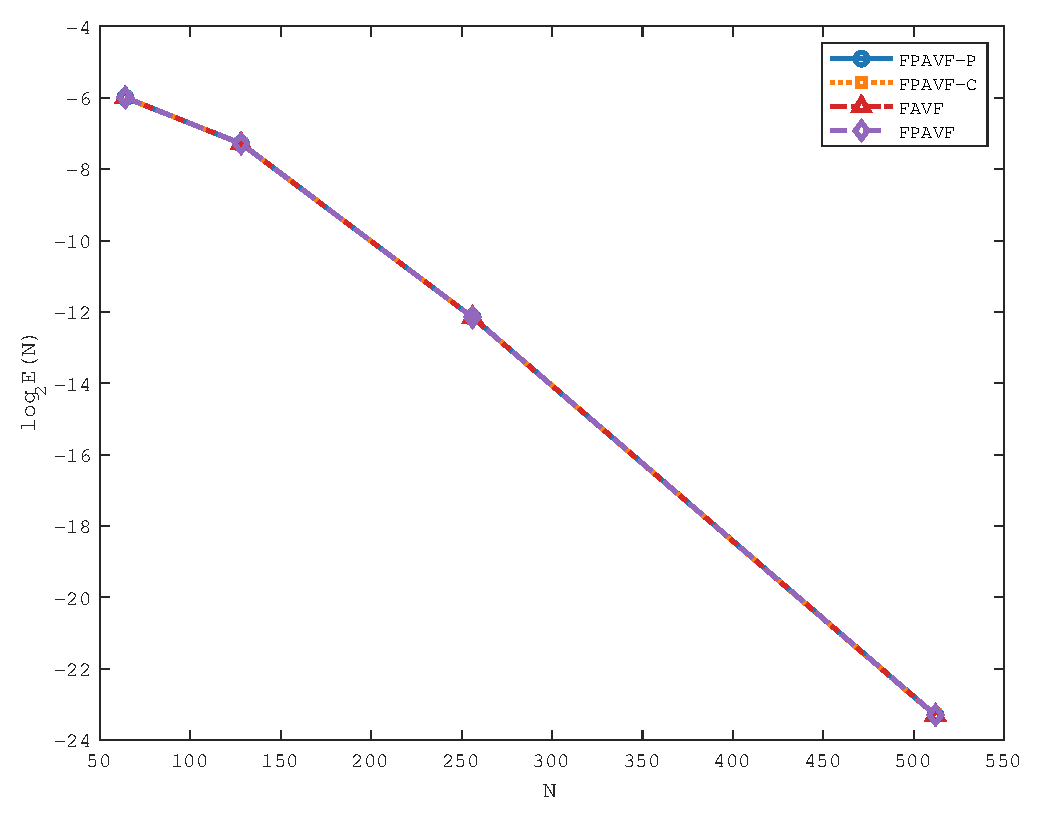
\includegraphics[width=0.35\textwidth]{./figure/exp1_s1.5.eps}
		%\centerline{($b$) Spatial accuracy with $\tau = 10^{-3}.$}
		}\subfigure[$N=128$]{ \centering
		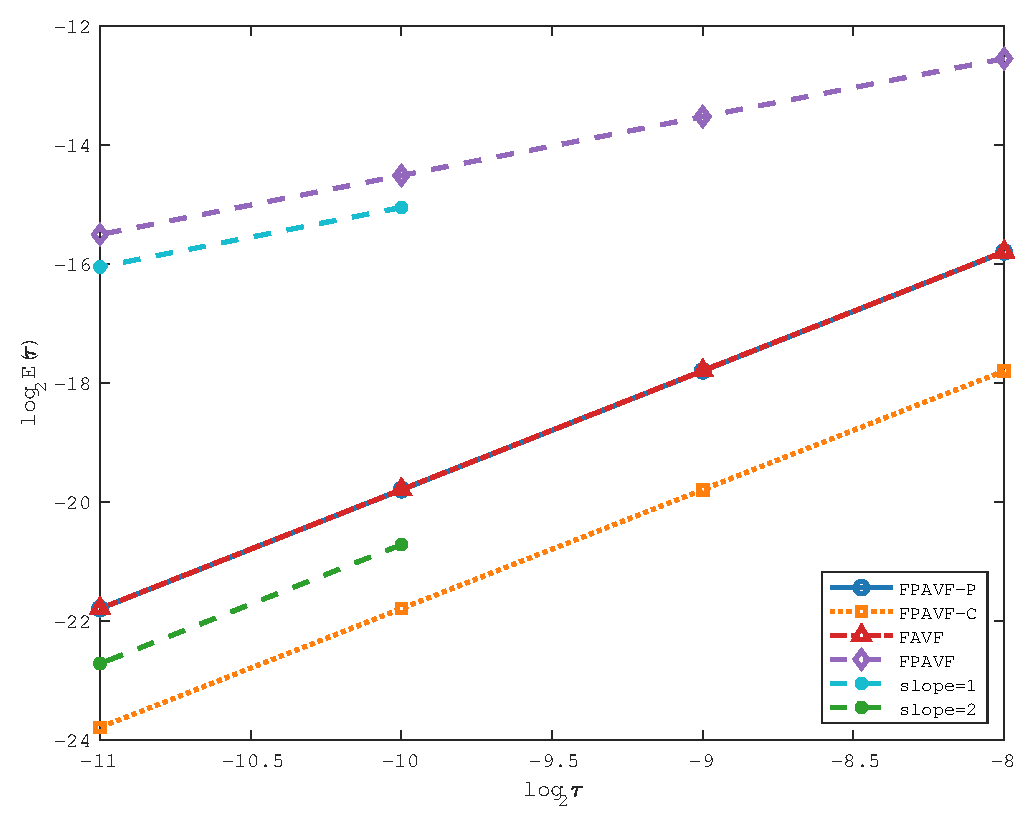
\includegraphics[width=0.35\textwidth]{./figure/exp1_t1.5.eps}
		%\centerline{($a$) Temporal accuracy with $N=128.$}
		}
		% \caption{Convergence orders of four schemes for Example \ref{exp_PAVF:2} with $\alpha=1.5$.}
		\caption{当$\alpha=1.5$时,算例 \ref{exp_PAVF:2} 中四种格式的收敛阶.}
		 \label{fig_PAVF:1}
		\end{center}
		\end{figure}
		
		\begin{figure}[H]
		\begin{center}
		\subfigure[$\tau=1/1000$]{ \centering
		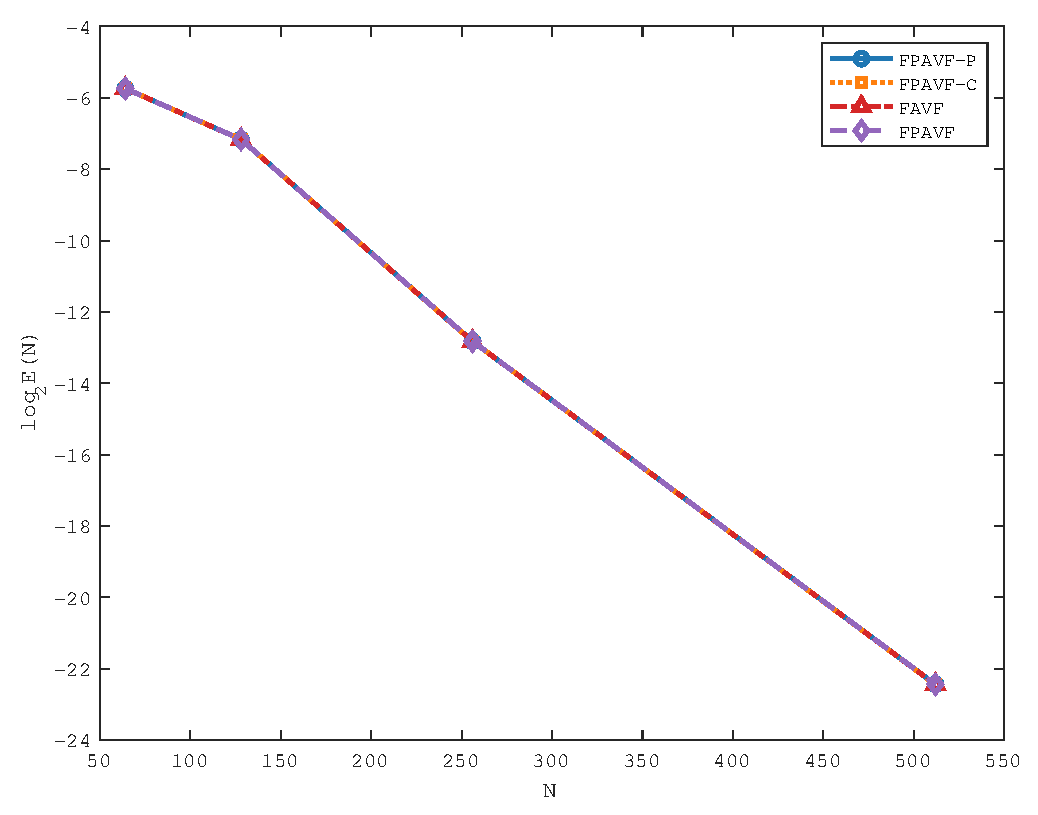
\includegraphics[width=0.35\textwidth]{./figure/exp1_s2.eps}
		%\centerline{($b$) Spatial accuracy with $\tau = 10^{-3}.$}
		}\subfigure[$N=128$]{ \centering
		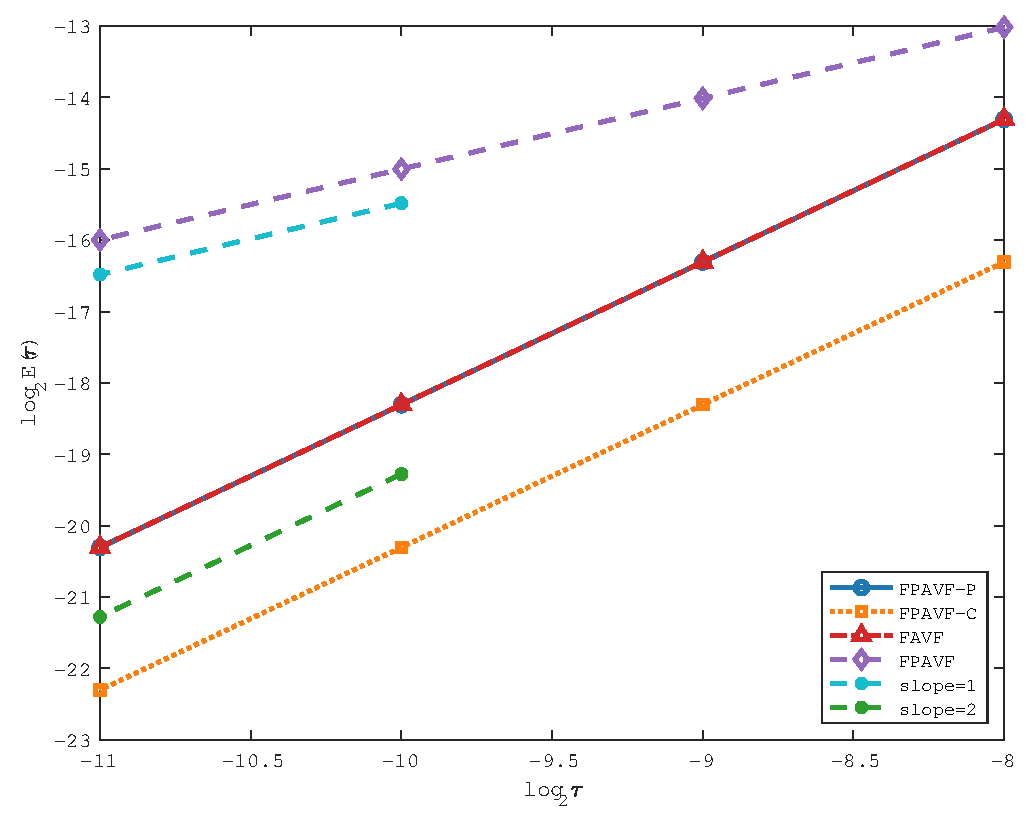
\includegraphics[width=0.35\textwidth]{./figure/exp1_t2.eps}
		%\centerline{($a$) Temporal accuracy with $N=128.$}
		}
		\caption{当$\alpha=2.0$时,算例 \ref{exp_PAVF:2} 中四种格式的收敛阶.}
		% \caption{Convergence orders of four schemes for Example \ref{exp_PAVF:2} with $\alpha=2.0$.} 
		\label{fig_PAVF:2}
		\end{center}
		\end{figure}


		\begin{figure}[H]
			\begin{center}
			\subfigure[$\alpha=1.3$]{ \centering
			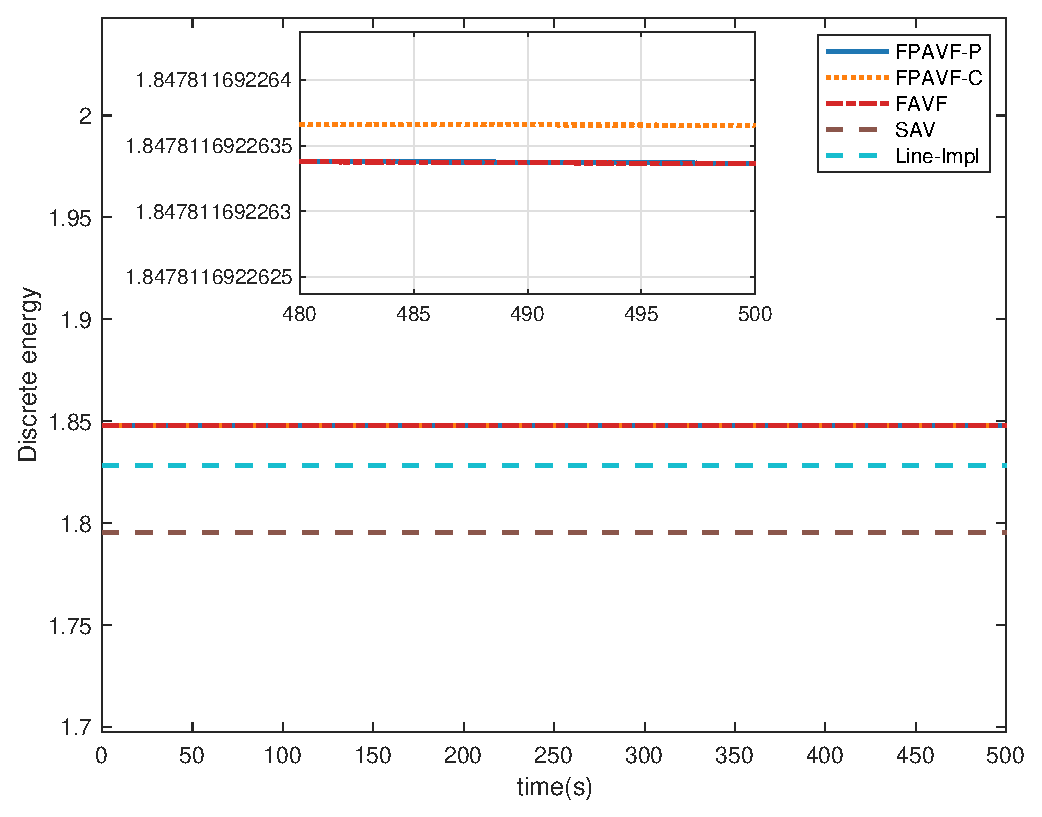
\includegraphics[width=0.4\textwidth]{./figure/exp1_H1.3.eps}
			%\centerline{($a$) $\alpha=1.3$}
			}\subfigure[$\alpha=1.6$]{ \centering
			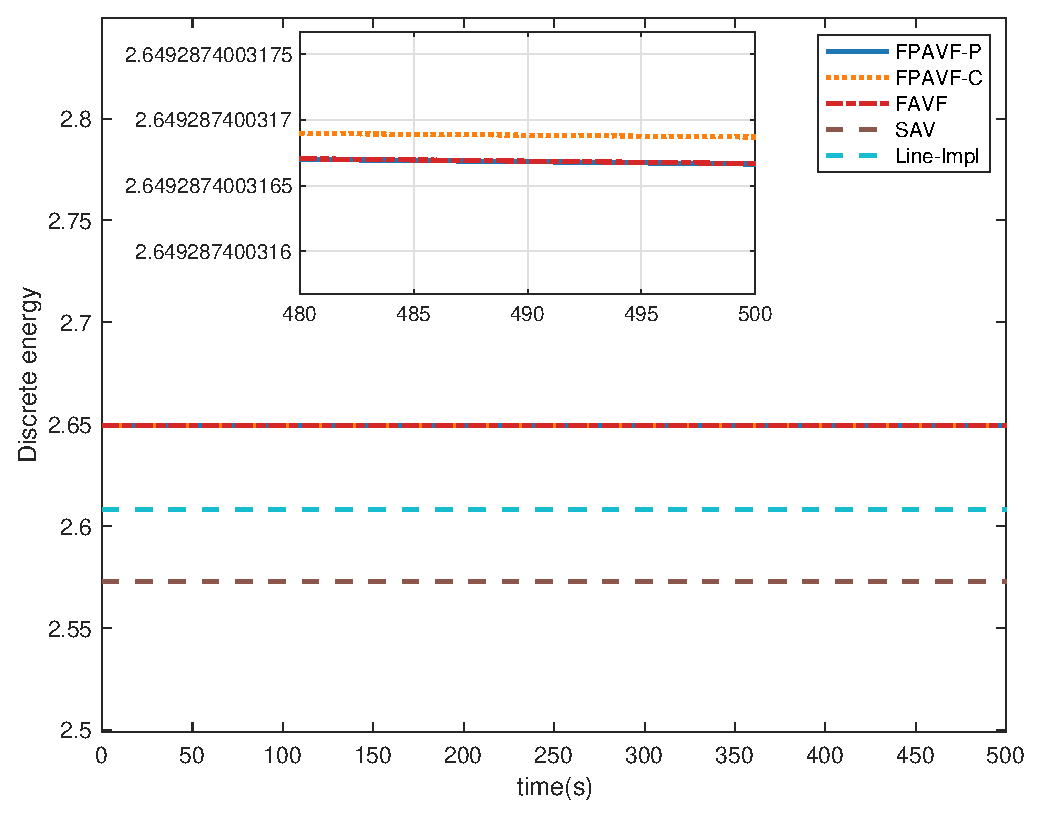
\includegraphics[width=0.4\textwidth]{./figure/exp1_H1.6.eps}
			%\centerline{($b$) $\alpha=1.6$}
			}\\
			\subfigure[$\alpha=1.9$]{ \centering
			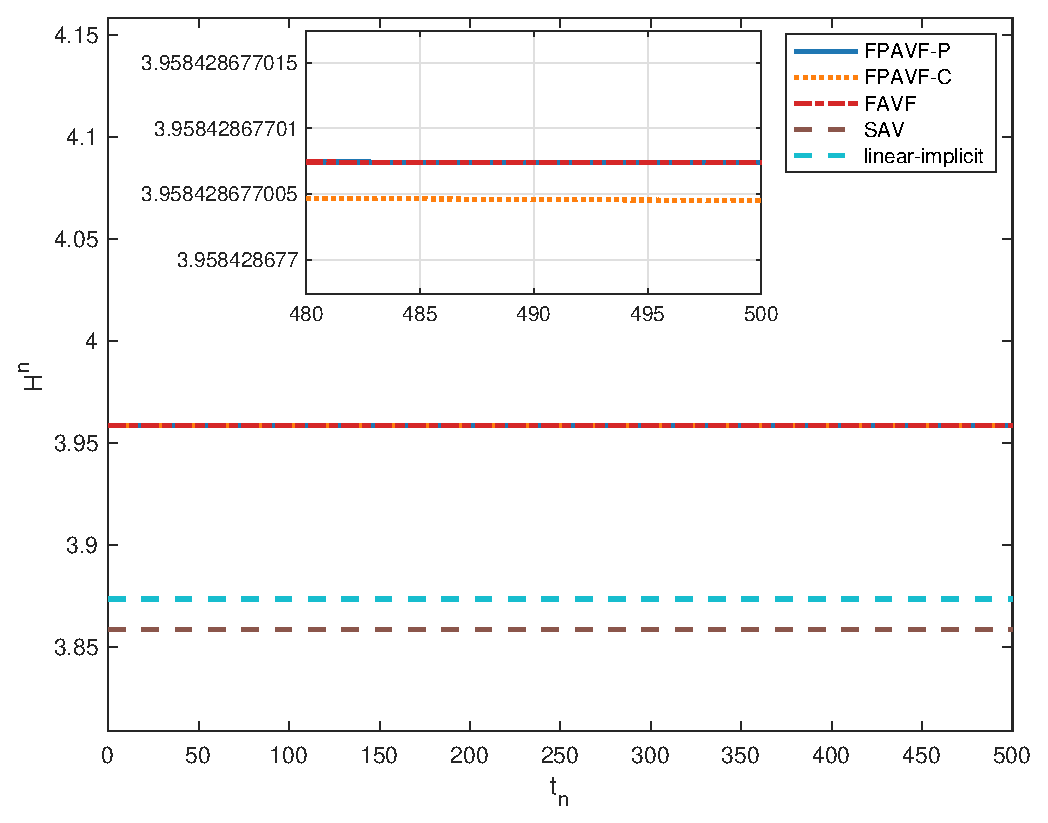
\includegraphics[width=0.4\textwidth]{./figure/exp1_H1.9.eps}
			%\centerline{($d$) $\alpha=2.0$}
			}\subfigure[$\alpha=2.0$]{ \centering
			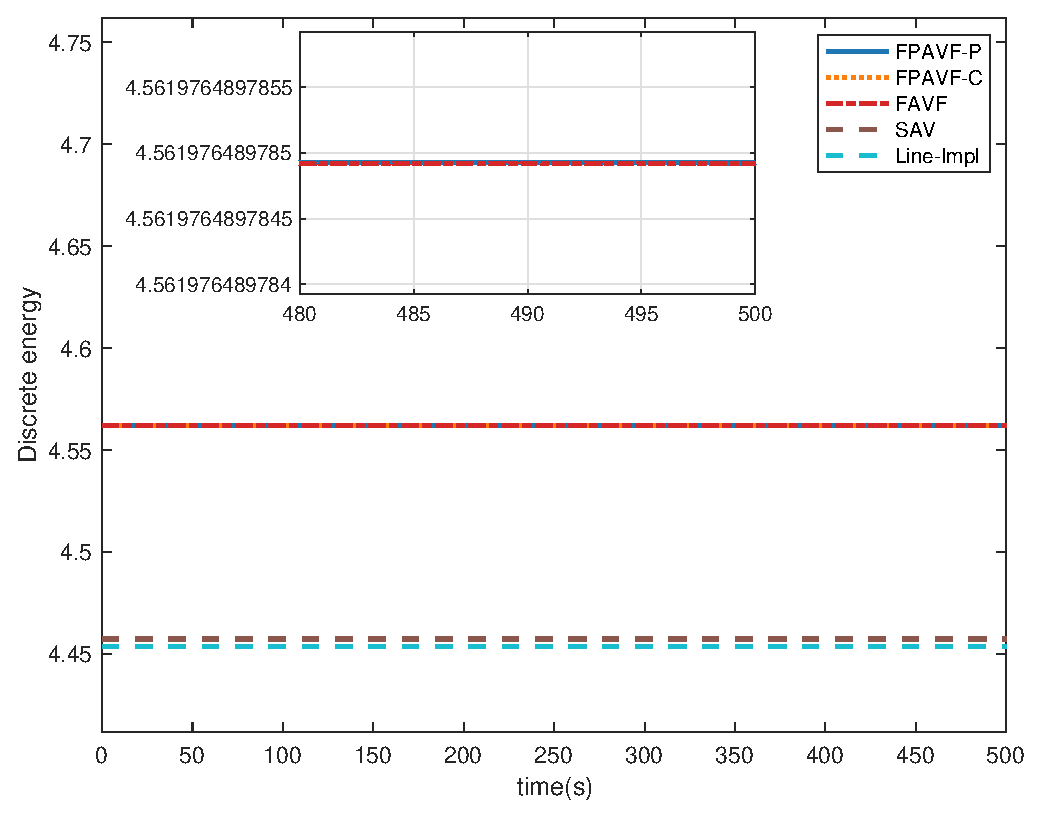
\includegraphics[width=0.4\textwidth]{./figure/exp1_H2.eps}
			%\centerline{($d$) $\alpha=2.0$}
			}
			% \caption{Discrete energy for different $\alpha$ in Example \ref{exp_PAVF:2} with $N = 512$ and $\tau=0.01$.}
			\caption{当 $N = 512, \tau=0.01$ 时,算例 \ref{exp_PAVF:2}取不同 $\alpha$ 的离散能量.}
			\label{fig_PAVF:3}
			\end{center}
			\end{figure}

图 \ref{fig_PAVF:3} 显示了几种格式在不同 $\alpha$ 值下,通过 $N=512$ 和 $\tau=0.01$ 计算的离散能量演化情况(T=500).
可以观察到,特别是在 $\alpha=2$ 时,FPAVF-P、FPAVF、FAVF 和 FPAVF-C 格式计算得到的离散能量均一致收敛到原始能量,
而 SAV 方法 \cite{chengConvergenceEnergyconservingScheme2022} 和三层线性隐式差分格式 \cite{ranLinearlyImplicitConservative2016} 的性能较差.
这一现象与后两者仅保持修正后的能量而不是原始能量的理论分析是一致的.

	类似地,图 \ref{fig_PAVF:4} 显示了在不同 $\alpha$ 值下,通过 $N=512$ 和 $\tau=0.01$ 计算的离散质量演化情况(T=500).需要强调的是 SAV 方法不具有质量守恒.
可以看到,FPAVF-P 格式收敛到原始质量,其他方法的性能相对较差,特别是 FAVF 格式,而三层线性隐式差分格式保持了修正后的质量.
此外,基于 FPAVF-C 格式的离散质量显示出小幅度的频繁振荡.


\begin{figure}[H]
	\begin{center}
	 \subfigure[$\alpha=1.3$]{ \centering
	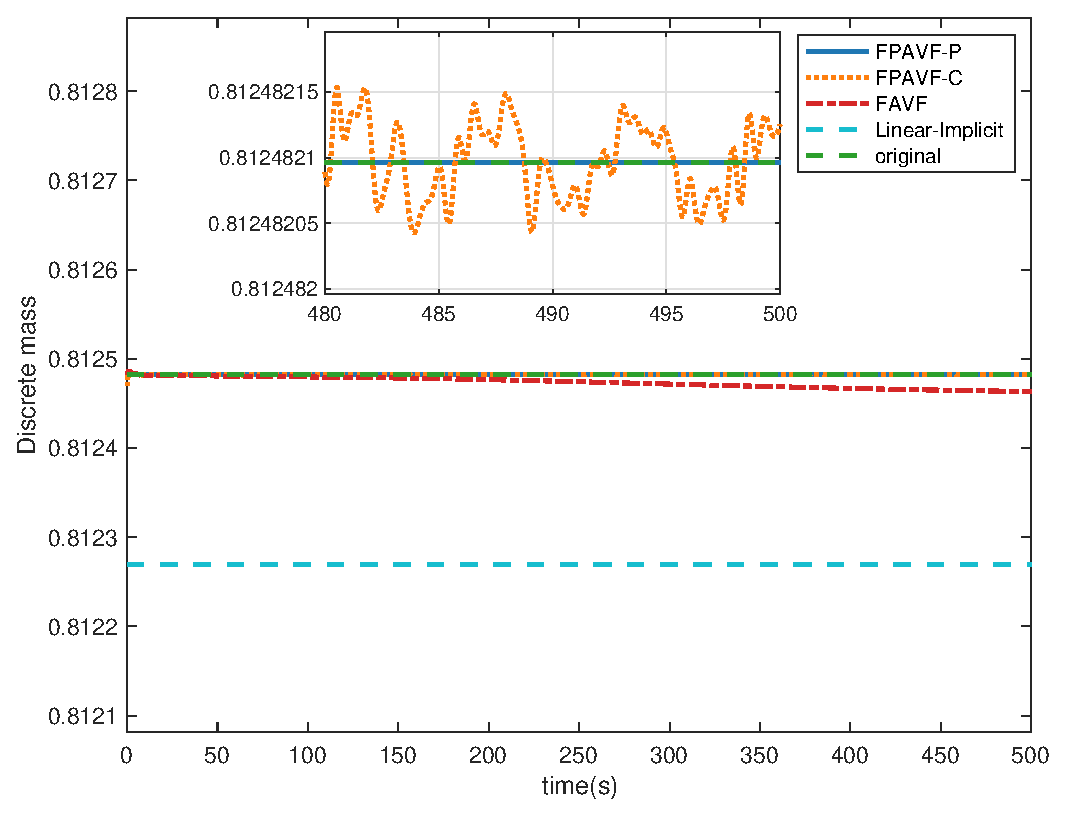
\includegraphics[width=0.4\textwidth]{./figure/exp1_M1.3.eps}
	%\centerline{($a$) $\alpha=1.3$}
	}\subfigure[$\alpha=1.6$]{ \centering
	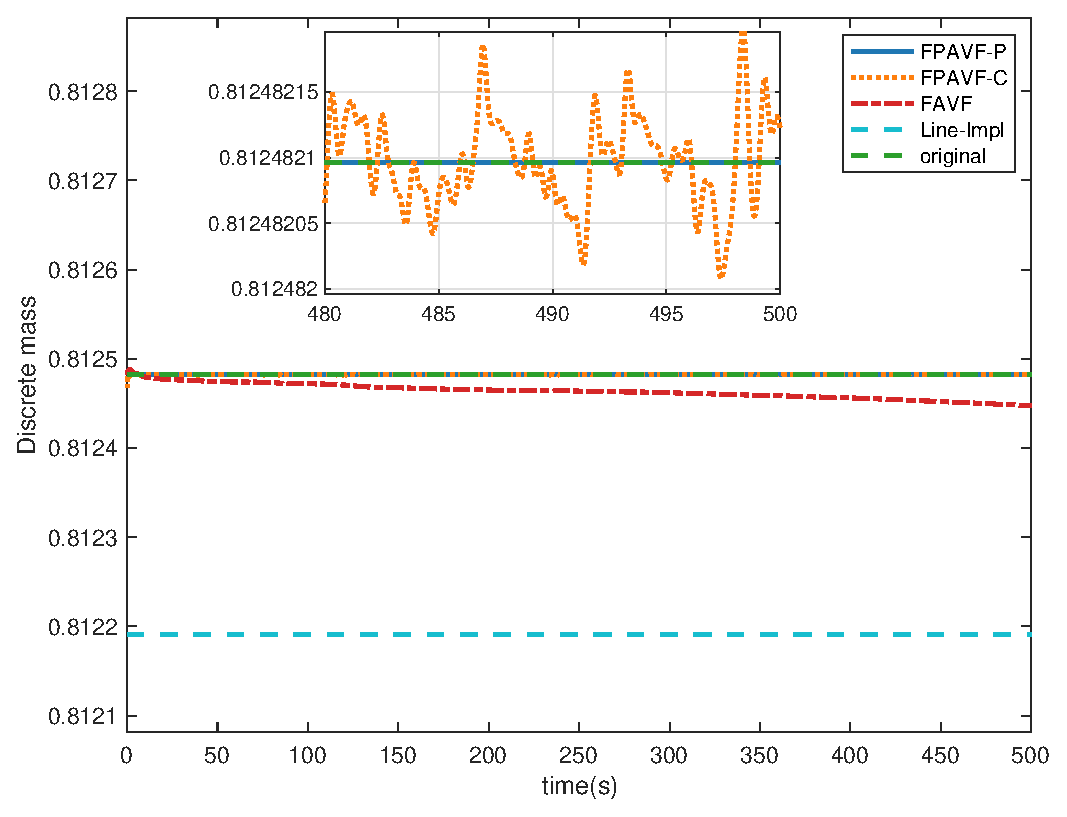
\includegraphics[width=0.4\textwidth]{./figure/exp1_M1.6.eps}
	%\centerline{($b$) $\alpha=1.6$}
	}\\
	 \subfigure[$\alpha=1.9$]{ \centering
	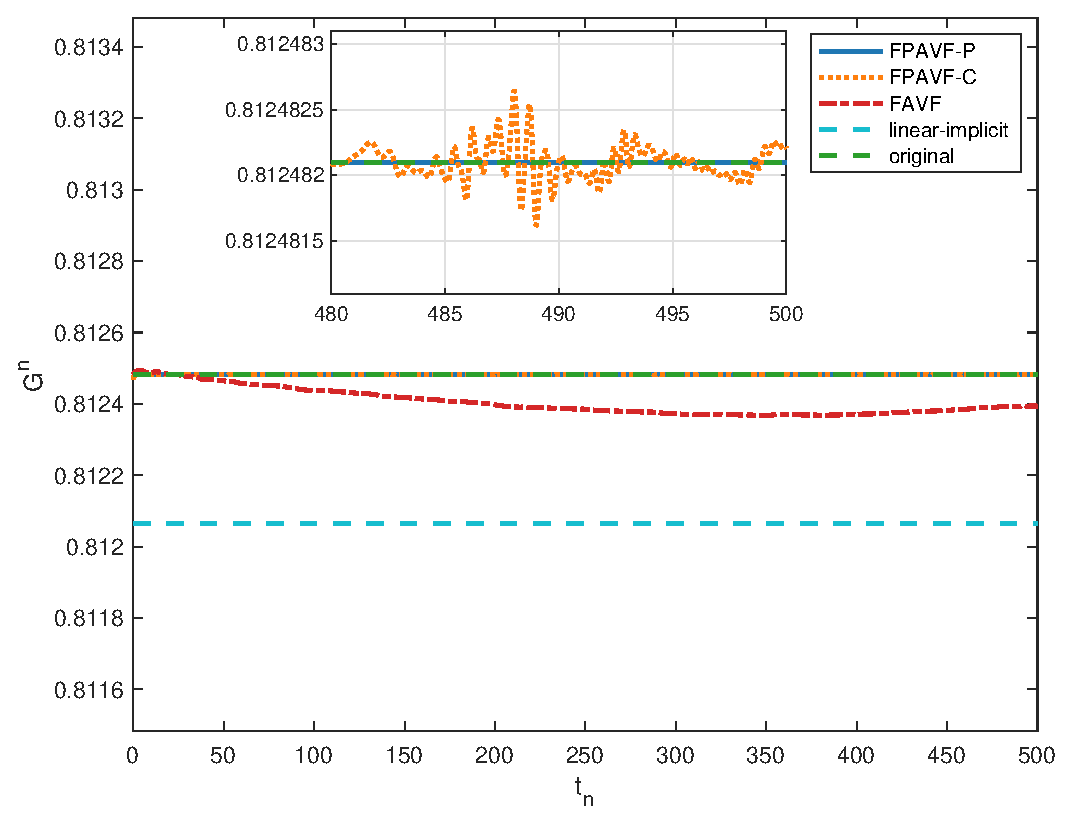
\includegraphics[width=0.4\textwidth]{./figure/exp1_M1.9.eps}
	%\centerline{($c$) $\alpha=1.9$}
	}\subfigure[$\alpha=2.0$]{ \centering
	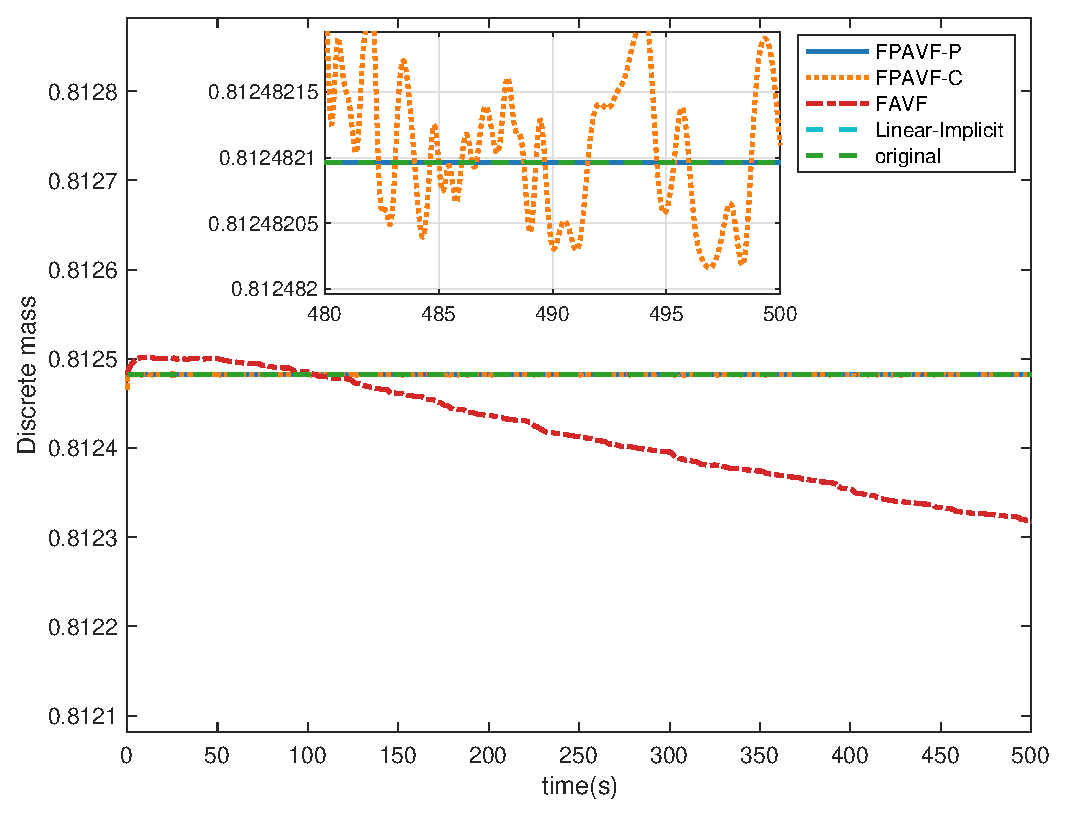
\includegraphics[width=0.4\textwidth]{./figure/exp1_M2.eps}
	%\centerline{($d$) $\alpha=2.0$}
	}
	% \caption{Discrete mass for different $\alpha$ in Example \ref{exp_PAVF:2} with $N = 512$ and $\tau=0.01$.}
	\caption{当 $N = 512, \tau=0.01$ 时,算例 \ref{exp_PAVF:2}取不同 $\alpha$ 的离散质量.}
	 \label{fig_PAVF:4}
	\end{center}
	\end{figure}

	更准确地说,表 \ref{tab_PAVF:1} 到表 \ref{tab_PAVF:4} 显示了不同 $\alpha$ 值下时刻 $t=t_{m}$ 时的离散能量 $H^{m}$ 和离散质量 $G^{m}$ 的值,这些值是通过取 $N=512$ 和 $\tau=0.01$ 获得的.从表 \ref{tab_PAVF:1} 可以看出,提出的四种格式均保持了原始能量,而 SAV 格式和三层线性隐式差分格式仅保持了修正后的能量.类似地,从表 \ref{tab_PAVF:2} 到表 \ref{tab_PAVF:4},观察到 FPAVF-P 格式收敛到原始质量,其他方法性能较差,而三层线性隐式差分格式仅保持了修正后的质量.

	
\begin{table}[H]\footnotesize
	\centering
	% \caption{Discrete energy $H^{m}$ at time $t=t_{m}$ for Example \ref{exp_PAVF:2} when $\alpha=2$.}
	\caption{当 $\alpha=2.0$ 时,算例 \ref{exp_PAVF:2} 在时刻 $t=t_{m}$ 的离散能量 $H^{m}$.}

	  \begin{tabular}{lllllll}
	  \toprule
       $t$   &FAVF   &FPAVF   &FPAVF-C   &SAV    &Linear-Implicit   &FPAVF-P\\
	%   \midrule
	%   0     &4.561976489785   &4.561976489785   &4.561976489785   &4.457414815200   &4.453861069486   &4.561976489785 \\
	%   10    &4.561976489785   &4.561976489785   &4.561976489785   &4.457414815200   &4.453861069486   &4.561976489785 \\
	%   100   &4.561976489785   &4.561976489785   &4.561976489782   &4.457414815197   &4.453861069489   &4.561976489785 \\
	%   200   &4.561976489785   &4.561976489785   &4.561976489779   &4.457414815195   &4.453861069492   &4.561976489785 \\
	%   300   &4.561976489785   &4.561976489785   &4.561976489776   &4.457414815192   &4.453861069494   &4.561976489785 \\
	%   400   &4.561976489785   &4.561976489785   &4.561976489772   &4.457414815190   &4.453861069497   &4.561976489785 \\
	%   500   &4.561976489785   &4.561976489785   &4.561976489768   &4.457414815187   &4.453861069500   &4.561976489785 \\
	%   \midrule
	\midrule
	0     &\textcolor{purple}{4.561976489}785   &\textcolor{purple}{4.561976489}785   &\textcolor{purple}{4.561976489}785   &\textcolor{purple}{4}.457414815200   &\textcolor{purple}{4}.453861069486   &\textcolor{purple}{4.561976489}785 \\
	10    &\textcolor{purple}{4.561976489}785   &\textcolor{purple}{4.561976489}785   &\textcolor{purple}{4.561976489}785   &\textcolor{purple}{4}.457414815200   &\textcolor{purple}{4}.453861069486   &\textcolor{purple}{4.561976489}785 \\
	100   &\textcolor{purple}{4.561976489}785   &\textcolor{purple}{4.561976489}785   &\textcolor{purple}{4.561976489}782   &\textcolor{purple}{4}.457414815197   &\textcolor{purple}{4}.453861069489   &\textcolor{purple}{4.561976489}785 \\
	200   &\textcolor{purple}{4.561976489}785   &\textcolor{purple}{4.561976489}785   &\textcolor{purple}{4.561976489}779   &\textcolor{purple}{4}.457414815195   &\textcolor{purple}{4}.453861069492   &\textcolor{purple}{4.561976489}785 \\
	300   &\textcolor{purple}{4.561976489}785   &\textcolor{purple}{4.561976489}785   &\textcolor{purple}{4.561976489}776   &\textcolor{purple}{4}.457414815192   &\textcolor{purple}{4}.453861069494   &\textcolor{purple}{4.561976489}785 \\
	400   &\textcolor{purple}{4.561976489}785   &\textcolor{purple}{4.561976489}785   &\textcolor{purple}{4.561976489}772   &\textcolor{purple}{4}.457414815190   &\textcolor{purple}{4}.453861069497   &\textcolor{purple}{4.561976489}785 \\
	500   &\textcolor{purple}{4.561976489}785   &\textcolor{purple}{4.561976489}785   &\textcolor{purple}{4.561976489}768   &\textcolor{purple}{4}.457414815187   &\textcolor{purple}{4}.453861069500   &\textcolor{purple}{4.561976489}785 \\
	\midrule
	  \multicolumn{7}{r}{Original energy:~4.56197648980619} \\
	  \bottomrule
	  \end{tabular}\label{tab_PAVF:1}%
  \end{table}%


\begin{table}[H]\footnotesize
	\centering
	% \caption{Discrete mass $G^{m}$ at time $t=t_{m}$ for Example \ref{exp_PAVF:2} when $\alpha=1.3$.}
	\caption{当 $\alpha=1.3$ 时,算例 \ref{exp_PAVF:2} 在时刻 $t=t_{m}$ 的离散质量 $G^{m}$.}
	  \begin{tabular}{llllll}
	  \toprule
$t$   &FAVF   &FPAVF   &FPAVF-C   &Linear-Implicit   &FPAVF-P\\
	%   \midrule
	%   0     &0.812482096011643   &0.812486108372853   &0.812481093228288   &0.812269212105079   &0.812482096009232 \\
	%   10    &0.812481652913507   &0.815448411130831   &0.812482228623069   &0.812269212105449   &0.812482096009234 \\
	%   100   &0.812479701090339   &0.815337307670638   &0.812482081439882   &0.812269212105119   &0.812482096009236 \\
	%   200   &0.812476755660814   &0.815352772611703   &0.812482091028916   &0.812269212105298   &0.812482096009256 \\
	%   300   &0.812471706145304   &0.815369448311709   &0.812482102752682   &0.812269212105193   &0.812482096009262 \\
	%   400   &0.812466871593141   &0.815375406648485   &0.812482112407629   &0.812269212105361   &0.812482096009263 \\
	%   500   &0.812463332390332   &0.815391313914498   &0.812482125179718   &0.812269212105409   &0.812482096009261 \\
	%   \midrule
	\midrule
	0     &\textcolor{purple}{0.81248}2096011643   &\textcolor{purple}{0.81248}6108372853   &\textcolor{purple}{0.81248}1093228288   &\textcolor{purple}{0.812}269212105079   &\textcolor{purple}{0.812482096009}232 \\
	10    &\textcolor{purple}{0.81248}1652913507   &\textcolor{purple}{0.81}5448411130831   &\textcolor{purple}{0.812482}228623069   &\textcolor{purple}{0.812}269212105449   &\textcolor{purple}{0.812482096009}234 \\
	100   &\textcolor{purple}{0.8124}79701090339   &\textcolor{purple}{0.81}5337307670638   &\textcolor{purple}{0.812482}081439882   &\textcolor{purple}{0.812}269212105119   &\textcolor{purple}{0.812482096009}236 \\
	200   &\textcolor{purple}{0.8124}76755660814   &\textcolor{purple}{0.81}5352772611703   &\textcolor{purple}{0.812482}091028916   &\textcolor{purple}{0.812}269212105298   &\textcolor{purple}{0.812482096009}256 \\
	300   &\textcolor{purple}{0.8124}71706145304   &\textcolor{purple}{0.81}5369448311709   &\textcolor{purple}{0.812482}102752682   &\textcolor{purple}{0.812}269212105193   &\textcolor{purple}{0.812482096009}262 \\
	400   &\textcolor{purple}{0.8124}66871593141   &\textcolor{purple}{0.81}5375406648485   &\textcolor{purple}{0.812482}112407629   &\textcolor{purple}{0.812}269212105361   &\textcolor{purple}{0.812482096009}263 \\
	500   &\textcolor{purple}{0.8124}63332390332   &\textcolor{purple}{0.81}5391313914498   &\textcolor{purple}{0.812482}125179718   &\textcolor{purple}{0.812}269212105409   &\textcolor{purple}{0.812482096009}261 \\
	\midrule
	  \multicolumn{6}{r}{Original mass:~0.812482096009503} \\
	  \bottomrule
	  \end{tabular}\label{tab_PAVF:2}%
  \end{table}%


\begin{table}[H]\footnotesize
	\centering
	% \caption{Discrete mass $G^{m}$ at time $t=t_{m}$ for Example \ref{exp_PAVF:2} when $\alpha=1.6$.}
	\caption{当 $\alpha=1.6$ 时,算例 \ref{exp_PAVF:2} 在时刻 $t=t_{m}$ 的离散质量 $G^{m}$.}
	\begin{tabular}{llllll}
	  \toprule
$t$   &FAVF   &FPAVF   &FPAVF-C   &Linear-Implicit   &FPAVF-P\\
	%   \midrule
	%   0     &0.812482096014526   &0.812487932904355   &0.812480637459791   &0.812191342790779   &0.812482096009232 \\
	%   10    &0.812479542844467   &0.815290680597744   &0.812482338980161   &0.812191342790869   &0.812482096009234 \\
	%   100   &0.812471993678066   &0.814964610988901   &0.812482077830270   &0.812191342790519   &0.812482096009245 \\
	%   200   &0.812465076996841   &0.814934135072654   &0.812482168949170   &0.812191342790438   &0.812482096009252 \\
	%   300   &0.812461964307183   &0.815026734196011   &0.812482132284732   &0.812191342790211   &0.812482096009255 \\
	%   400   &0.812456227758388   &0.815045189971354   &0.812482132454783   &0.812191342790067   &0.812482096009255 \\
	%   500   &0.812447472460440   &0.815097180030255   &0.812482122664758   &0.812191342789578   &0.812482096009251 \\
	%   \midrule
	\midrule
	0     &\textcolor{purple}{0.81248}2096014526   &\textcolor{purple}{0.81248}7932904355   &\textcolor{purple}{0.81248}0637459791   &\textcolor{purple}{0.812}191342790779   &\textcolor{purple}{0.812482096009}232 \\
	10    &\textcolor{purple}{0.8124}79542844467   &\textcolor{purple}{0.81}5290680597744   &\textcolor{purple}{0.812482}338980161   &\textcolor{purple}{0.812}191342790869   &\textcolor{purple}{0.812482096009}234 \\
	100   &\textcolor{purple}{0.8124}71993678066   &\textcolor{purple}{0.81}4964610988901   &\textcolor{purple}{0.812482}077830270   &\textcolor{purple}{0.812}191342790519   &\textcolor{purple}{0.812482096009}245 \\
	200   &\textcolor{purple}{0.8124}65076996841   &\textcolor{purple}{0.81}4934135072654   &\textcolor{purple}{0.812482}168949170   &\textcolor{purple}{0.812}191342790438   &\textcolor{purple}{0.812482096009}252 \\
	300   &\textcolor{purple}{0.8124}61964307183   &\textcolor{purple}{0.81}5026734196011   &\textcolor{purple}{0.812482}132284732   &\textcolor{purple}{0.812}191342790211   &\textcolor{purple}{0.812482096009}255 \\
	400   &\textcolor{purple}{0.8124}56227758388   &\textcolor{purple}{0.81}5045189971354   &\textcolor{purple}{0.812482}132454783   &\textcolor{purple}{0.812}191342790067   &\textcolor{purple}{0.812482096009}255 \\
	500   &\textcolor{purple}{0.8124}47472460440   &\textcolor{purple}{0.81}5097180030255   &\textcolor{purple}{0.812482}122664758   &\textcolor{purple}{0.812}191342789578   &\textcolor{purple}{0.812482096009}251 \\
	\midrule
	  \multicolumn{6}{r}{Original mass:~0.812482096009503} \\
	  \bottomrule
	  \end{tabular}\label{tab_PAVF:3}%
  \end{table}%


\begin{table}[H]\footnotesize
	\centering
	% \caption{Discrete mass $G^{m}$ at time $t=t_{m}$ for Example \ref{exp_PAVF:2} when $\alpha=2$.}
	\caption{当 $\alpha=2.0$ 时,算例 \ref{exp_PAVF:2} 在时刻 $t=t_{m}$ 的离散质量 $G^{m}$.}
	\begin{tabular}{llllll}
	  \toprule
$t$   &FAVF   &FPAVF   &FPAVF-C   &Linear-Implicit   &FPAVF-P\\
	%   \midrule
	%   0     &0.812482096027426   &0.812492566135382   &0.812479480708946   &0.812007279829162   &0.812482096009232 \\
	%   10    &0.812501574603936   &0.815690689466538   &0.812482208549750   &0.812007279829185   &0.812482096009233 \\
	%   100   &0.812485179319911   &0.815559529804266   &0.812482224295188   &0.812007279829068   &0.812482096009234 \\
	%   200   &0.812436598720768   &0.815737264057778   &0.812482177481325   &0.812007279828906   &0.812482096009234 \\
	%   300   &0.812395565737519   &0.815914179675223   &0.812482122649446   &0.812007279828999   &0.812482096009235 \\
	%   400   &0.812353830841431   &0.816227202656059   &0.812482101787071   &0.812007279828969   &0.812482096009235 \\
	%   500   &0.812317849493374   &0.816336221770707   &0.812482109657662   &0.812007279829037   &0.812482096009234 \\
	%   \midrule
	\midrule
	0     &\textcolor{purple}{0.81248}2096027426   &\textcolor{purple}{0.8124}92566135382   &\textcolor{purple}{0.8124}79480708946   &\textcolor{purple}{0.812}007279829162   &\textcolor{purple}{0.812482096009}232 \\
	10    &\textcolor{purple}{0.8125}01574603936   &\textcolor{purple}{0.81}5690689466538   &\textcolor{purple}{0.812482}208549750   &\textcolor{purple}{0.812}007279829185   &\textcolor{purple}{0.812482096009}233 \\
	100   &\textcolor{purple}{0.81248}5179319911   &\textcolor{purple}{0.81}5559529804266   &\textcolor{purple}{0.812482}224295188   &\textcolor{purple}{0.812}007279829068   &\textcolor{purple}{0.812482096009}234 \\
	200   &\textcolor{purple}{0.8124}36598720768   &\textcolor{purple}{0.81}5737264057778   &\textcolor{purple}{0.812482}177481325   &\textcolor{purple}{0.812}007279828906   &\textcolor{purple}{0.812482096009}234 \\
	300   &\textcolor{purple}{0.812}395565737519   &\textcolor{purple}{0.81}5914179675223   &\textcolor{purple}{0.812482}122649446   &\textcolor{purple}{0.812}007279828999   &\textcolor{purple}{0.812482096009}235 \\
	400   &\textcolor{purple}{0.812}353830841431   &\textcolor{purple}{0.81}6227202656059   &\textcolor{purple}{0.812482}101787071   &\textcolor{purple}{0.812}007279828969   &\textcolor{purple}{0.812482096009}235 \\
	500   &\textcolor{purple}{0.812}317849493374   &\textcolor{purple}{0.81}6336221770707   &\textcolor{purple}{0.812482}109657662   &\textcolor{purple}{0.812}007279829037   &\textcolor{purple}{0.812482096009}234 \\
	\midrule
	  \multicolumn{6}{r}{Original mass:~0.812482096009503} \\
	  \bottomrule
	  \end{tabular}\label{tab_PAVF:4}%
  \end{table}%

  对于 $\alpha\neq 2$的原始能量计算比较困难, 于是从相对误差的角度验证了离散守恒定律,见图 \ref{fig_PAVF:5} - \ref{fig_PAVF:6}.
  同样,图中显示 FPAVF-P 格式在保持原始质量守恒方面具有最佳性能.随着 $\alpha$ 的增加,它在保持原始能量方面的性能将更好.这些观察与之前的理论结果一致.

  \begin{figure}[H]
	\begin{center}
	 \subfigure[$\alpha=1.3$]{ \centering
	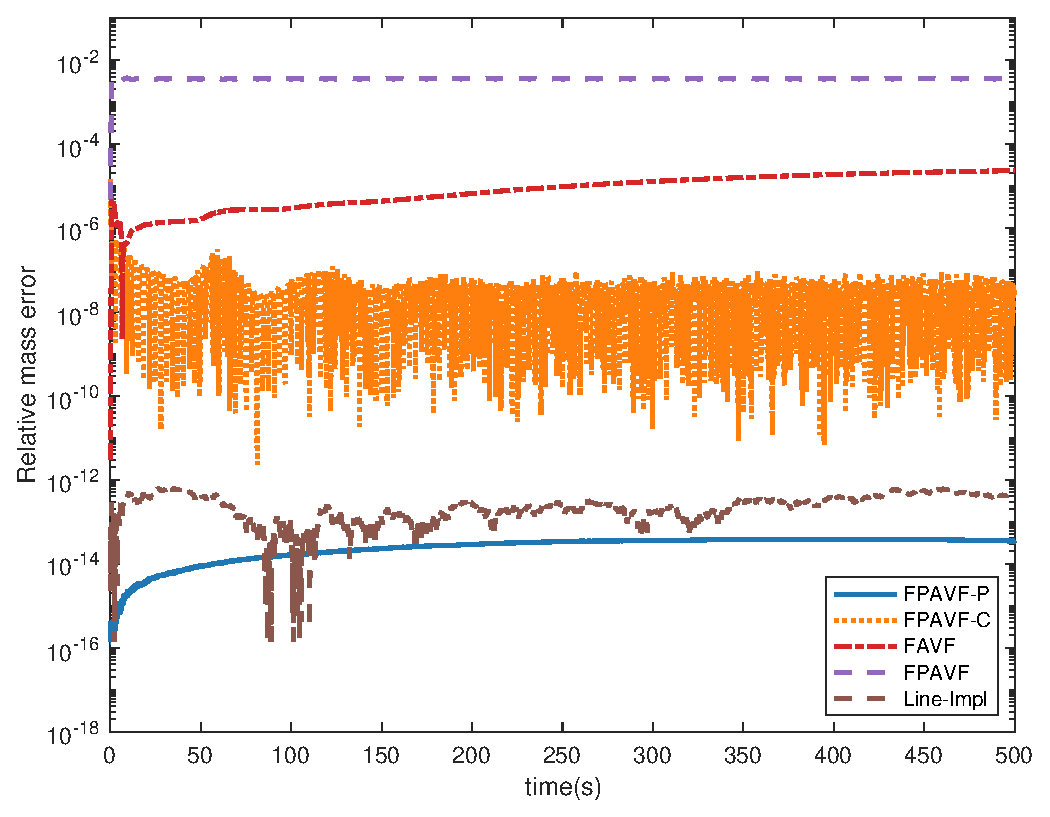
\includegraphics[width=0.3\textwidth]{./figure/exp1_RM1.3.eps}
	%\centerline{($a$) $\alpha=1.3$}
	}\subfigure[$\alpha=1.6$]{ \centering
	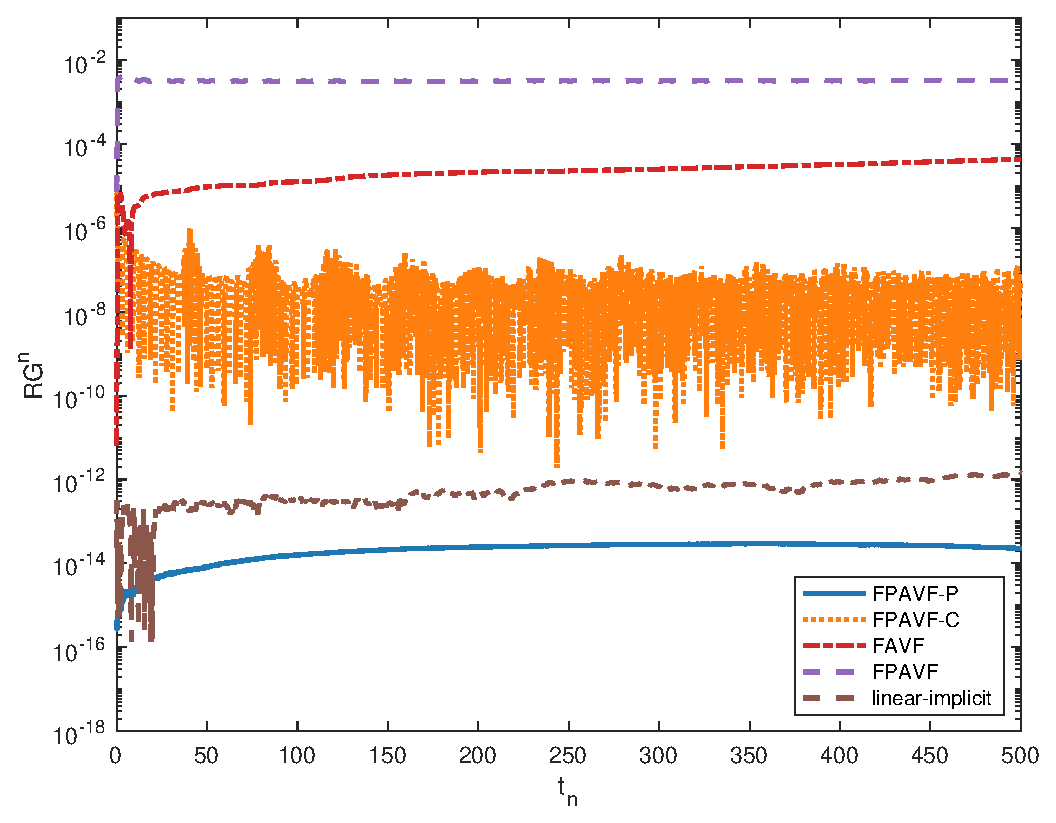
\includegraphics[width=0.3\textwidth]{./figure/exp1_RM1.6.eps}
	%\centerline{($b$) $\alpha=1.6$}
	}\subfigure[$\alpha=1.9$]{ \centering
	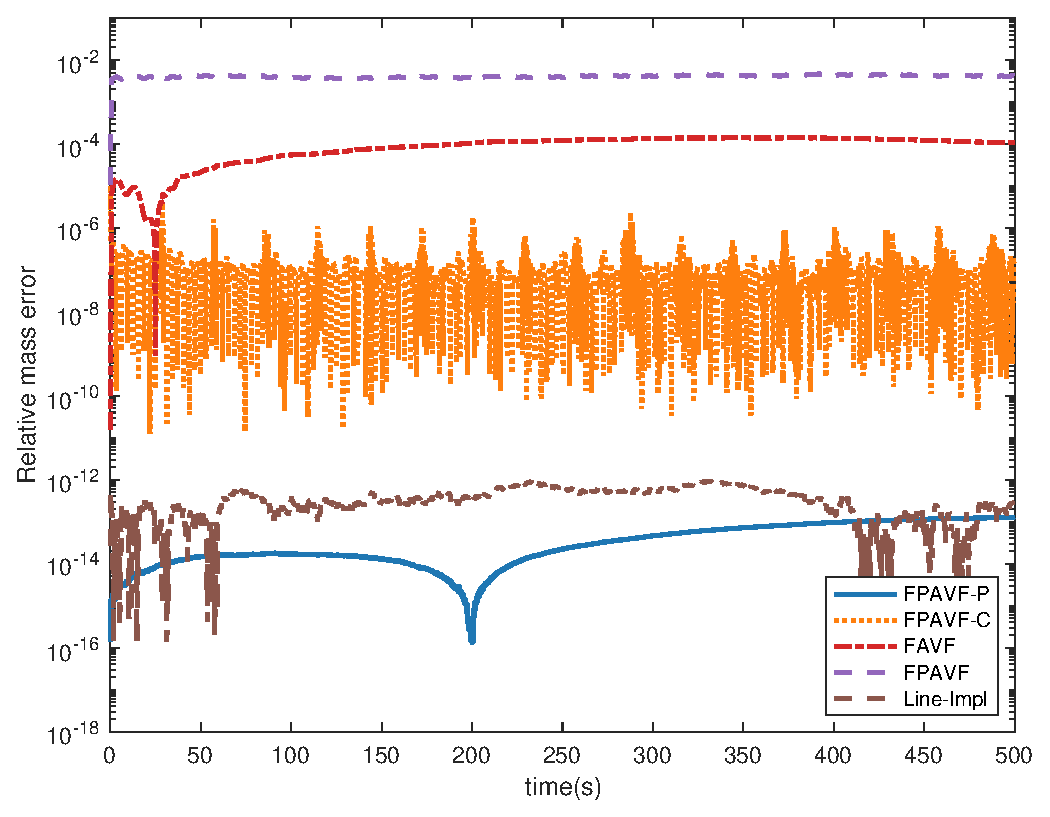
\includegraphics[width=0.3\textwidth]{./figure/exp1_RM1.9.eps}
	%\centerline{($c$) $\alpha=1.9$}
	}
	% \caption{The relative errors of discrete mass for different $\alpha$ in Example \ref{exp_PAVF:2} with $N = 512$ and $\tau=0.01$.}
	\caption{当 $N = 512, \tau=0.01$ 时,算例 \ref{exp_PAVF:2}取不同 $\alpha$ 的相对质量误差}
	\label{fig_PAVF:5}
	\end{center}
	\end{figure}
	
	\begin{figure}[H]
	\begin{center}
	 \subfigure[$\alpha=1.3$]{ \centering
	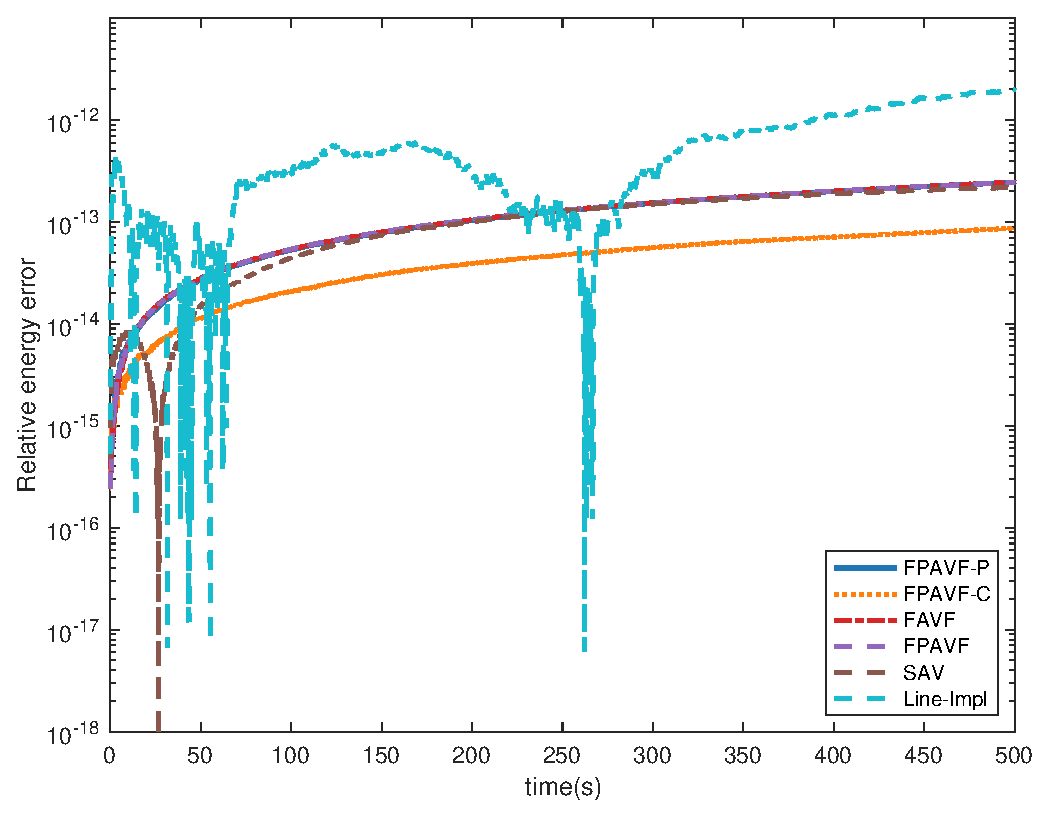
\includegraphics[width=0.3\textwidth]{./figure/exp1_RH1.3.eps}
	%\centerline{($a$) $\alpha=1.3$}
	}\subfigure[$\alpha=1.6$]{ \centering
	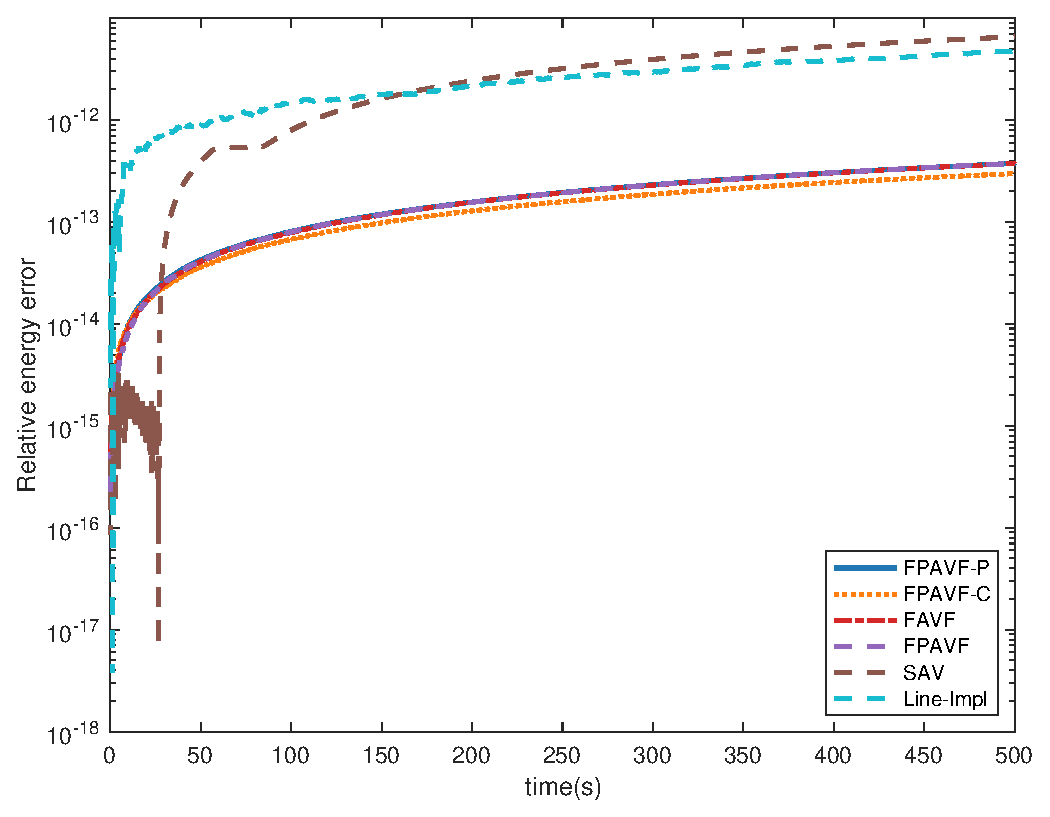
\includegraphics[width=0.3\textwidth]{./figure/exp1_RH1.6.eps}
	%\centerline{($b$) $\alpha=1.6$}
	} \subfigure[$\alpha=1.9$]{ \centering
	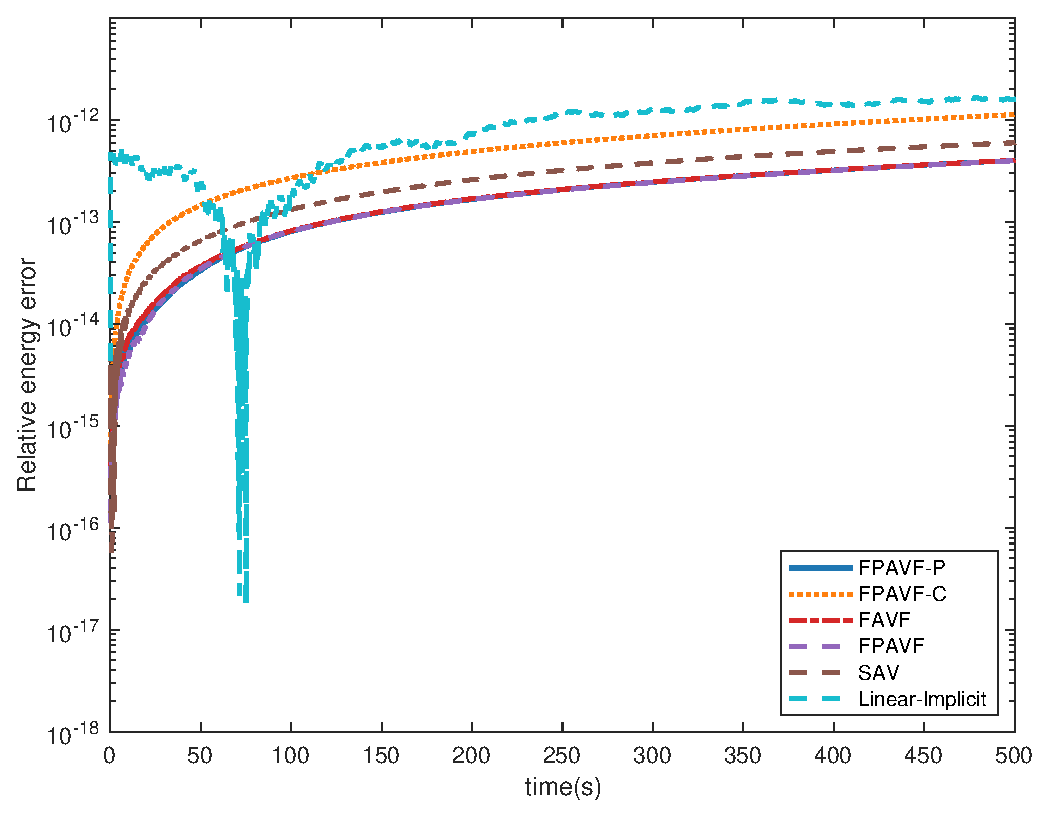
\includegraphics[width=0.3\textwidth]{./figure/exp1_RH1.9.eps}
	%\centerline{($c$) $\alpha=1.9$}
	} 
	% \caption{The relative errors of discrete energy for different $\alpha$ in Example \ref{exp_PAVF:2} with $N = 512$ and $\tau=0.01$.} 
	\caption{当 $N = 512, \tau=0.01$ 时,算例 \ref{exp_PAVF:2}取不同 $\alpha$ 的相对能量误差}\label{fig_PAVF:6}
	\end{center}
	\end{figure}
	\begin{example}\label{exp_PAVF:4}
		考虑带有初始值的二维非线性分数薛定谔波动方程 \eqref{eq_SAVRRK:1}-\eqref{eq_SAVRRK:3}
		\begin{equation}\label{eq_PAVF_110}
		u(x,y, 0)=\mbox{sech}\left(x^2+y^2\right), u_t(x,y, 0)=\sin (x+y) \mbox{sech}\left(-2(x^2+y^2)\right), (x,y,t)\in  \Omega\times[0, T],
		\end{equation}
		其中 $\Omega=[-5,5] \times[-5,5]$.
		\end{example}

	类似于一维情况, 首先计算 FPAVF-P、FPAVF、FAVF 和 FPAVF-C 格式在 $T=1$时 $\alpha=1.5$ 和 $\alpha=2.0$  的收敛阶.
	如图 \ref{fig_PAVF:7} - \ref{fig_PAVF:8} 所示.可以清晰地观察到这四种格式在空间方向都具有谱精度,而 FPAVF 格式在时间方向表现出一阶精度,其他格式在时间方向表现出二阶精度.

	
\begin{figure}[H]
	\begin{center}
	\subfigure[$\tau=1/1000$]{ \centering
	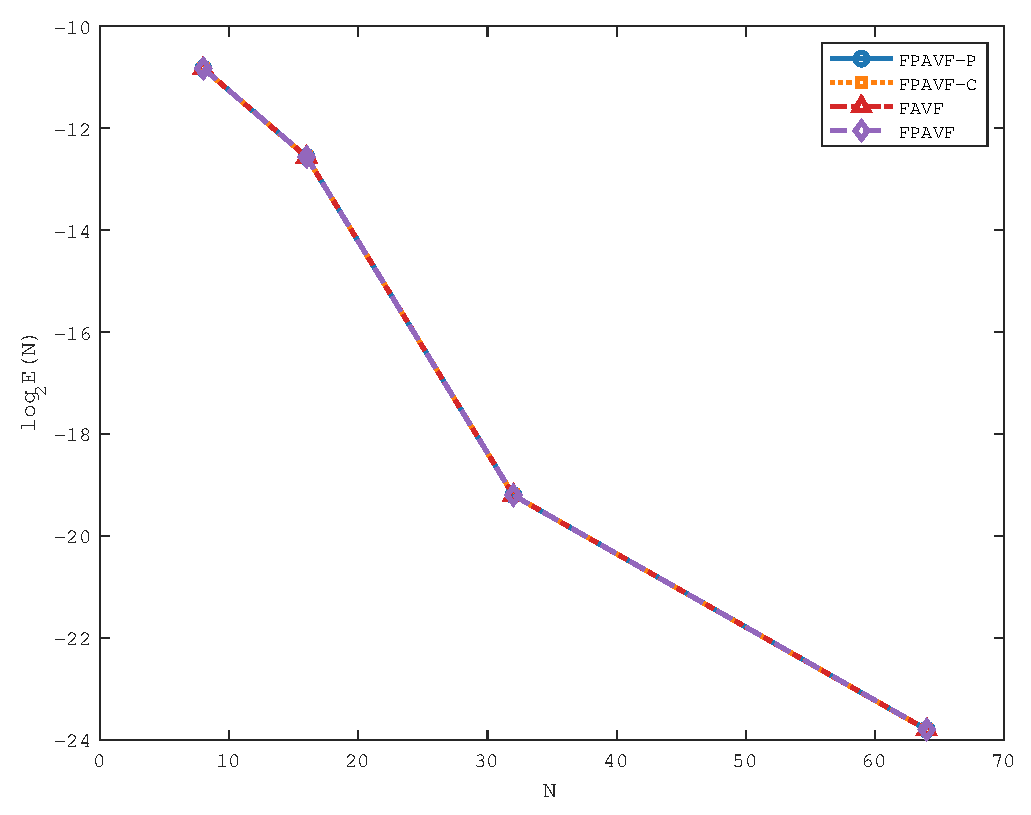
\includegraphics[width=0.35\textwidth]{./figure/exp2_s1.5.eps}
	%\centerline{($b$) Spatial accuracy with $\tau = 10^{-3}.$}
	}\subfigure[$N=16$]{ \centering
	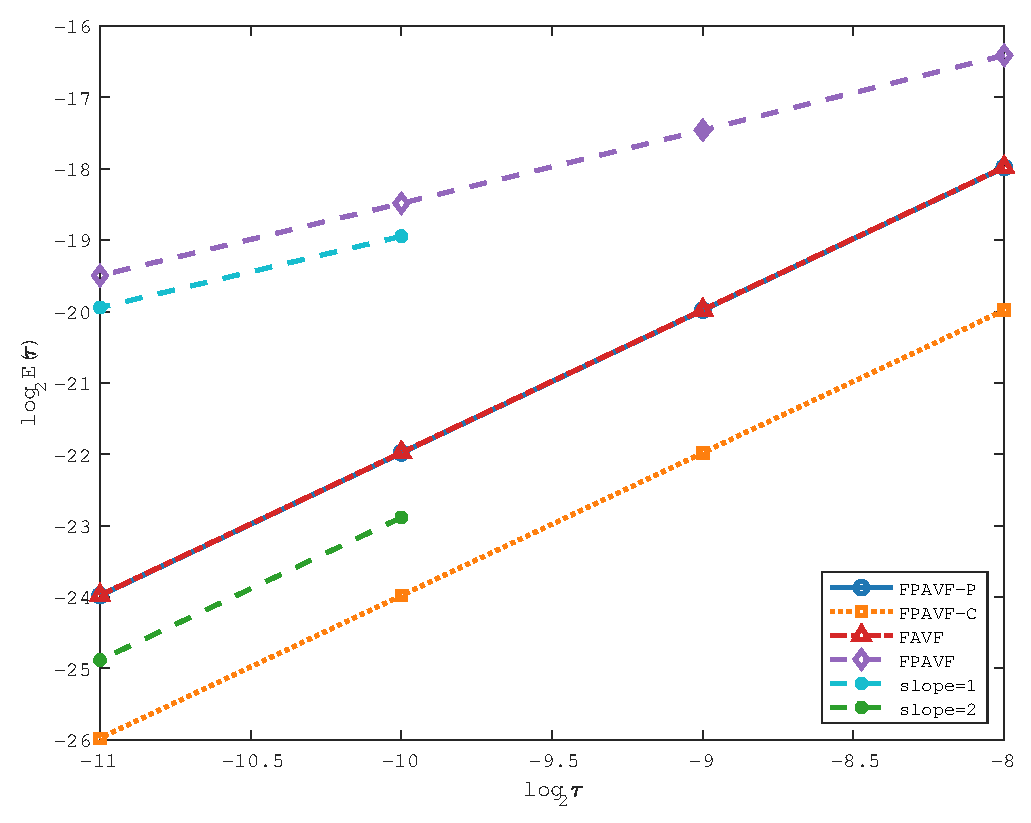
\includegraphics[width=0.35\textwidth]{./figure/exp2_t1.5.eps}
	%\centerline{($a$) Temporal accuracy with $N=128.$}
	}
	% \caption{Convergence orders of four schemes for Example \ref{exp_PAVF:4} with $\alpha=1.5$.} 
	\caption{当$\alpha=1.5$时,算例 \ref{exp_PAVF:4} 中四种格式的收敛阶.}
	\label{fig_PAVF:7}
	\end{center}
	\end{figure}
	
	\begin{figure}[H]
	\begin{center}
	\subfigure[$\tau=1/1000$]{ \centering
	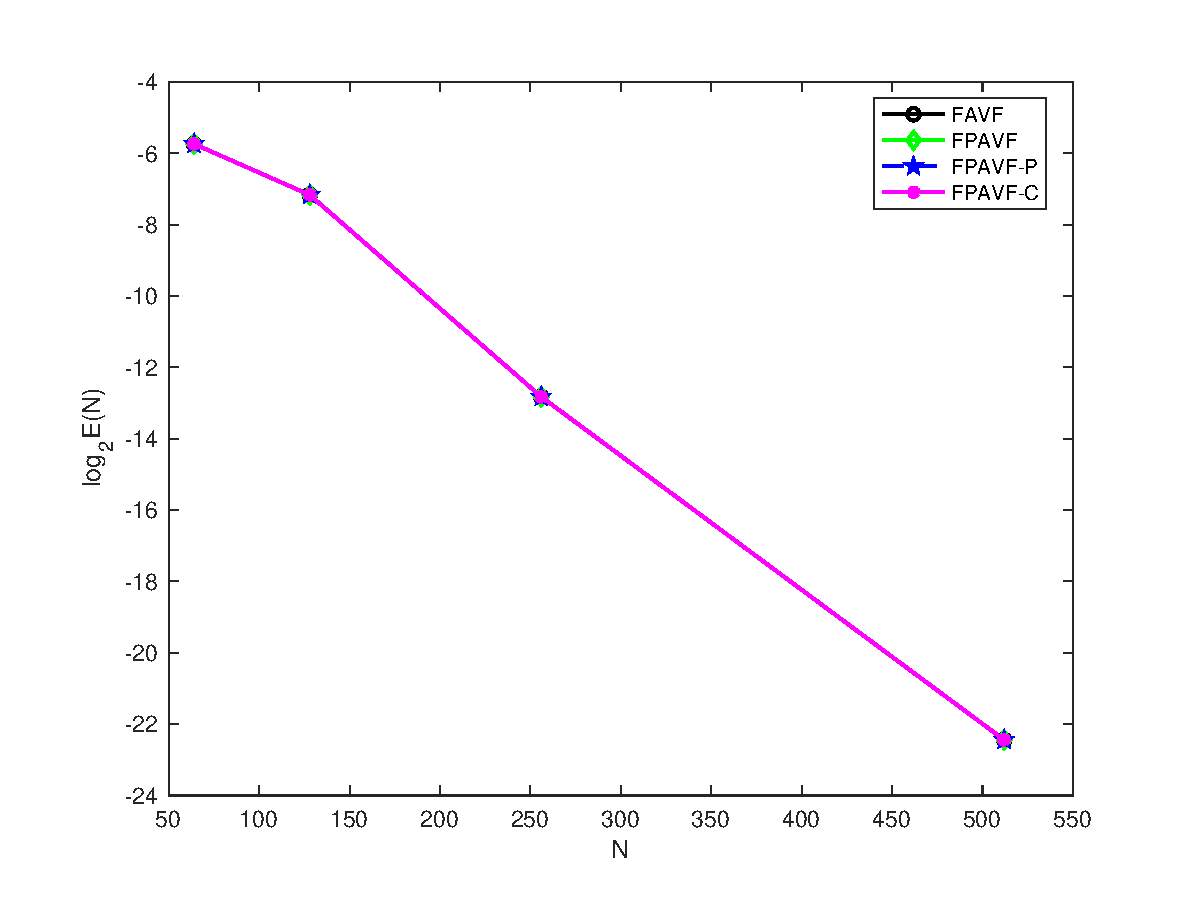
\includegraphics[width=0.35\textwidth]{./figure/exp2_s2.eps}
	%\centerline{($b$) Spatial accuracy with $\tau = 10^{-3}.$}
	}\subfigure[$N=16$]{ \centering
	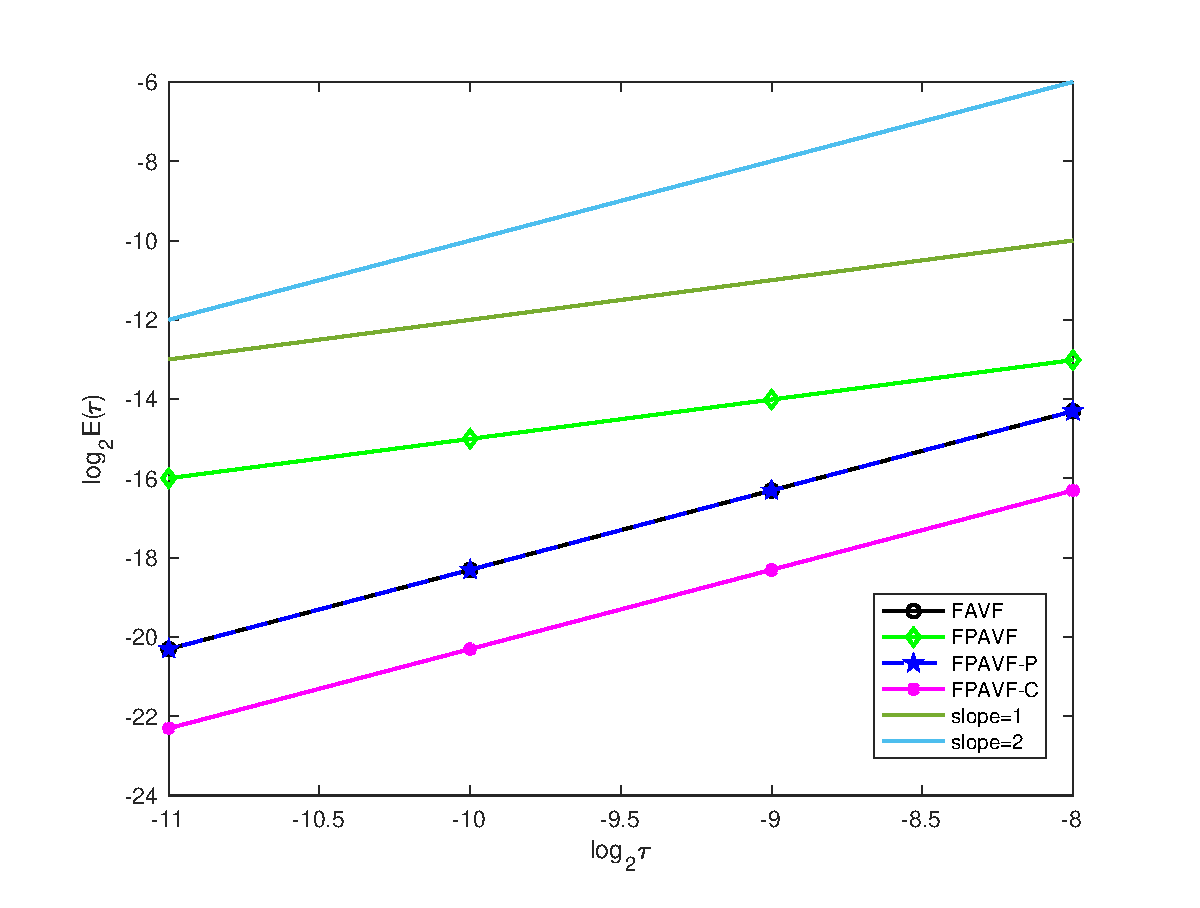
\includegraphics[width=0.35\textwidth]{./figure/exp2_t2.eps}
	%\centerline{($a$) Temporal accuracy with $N=128.$}
	}
	% \caption{Convergence orders of four schemes for Example \ref{exp_PAVF:4} with $\alpha=2.0$.}
	\caption{当$\alpha=2.0$时,算例 \ref{exp_PAVF:4} 中四种格式的收敛阶.}
	 \label{fig_PAVF:8}
	\end{center}
	\end{figure}

	注意到原始质量 $G(t)$ 与 $\alpha$ 无关,通过高斯数值积分,得到了任何 $\alpha$ 下的原始质量 $G(0)=3.14159265323701$.
	类似地,可以得到 $\alpha=2$ 时的原始能量 $E(0)=3.22697078976648$.

\begin{figure}[H]
	\begin{center}
	 \subfigure[$\alpha=1.3$]{ \centering
	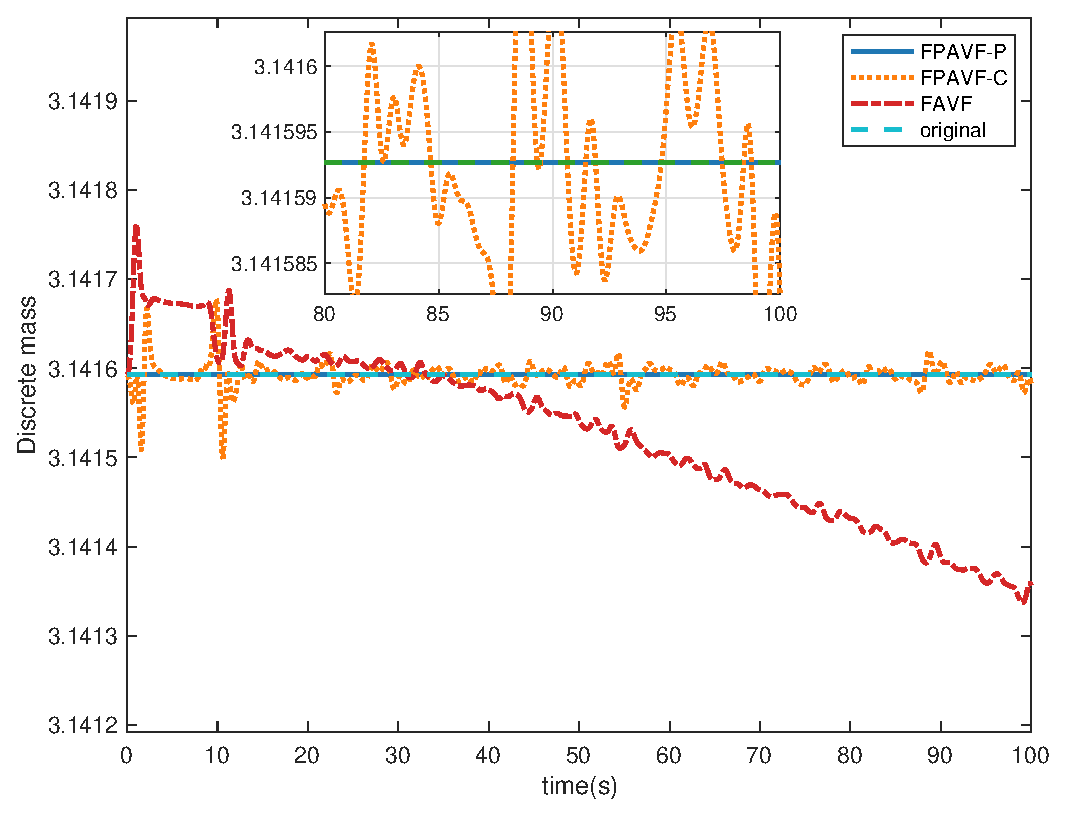
\includegraphics[width=0.3\textwidth]{./figure/exp2_M1.3.eps}
	%\centerline{($a$) $\alpha=1.3$}
	}\subfigure[$\alpha=1.6$]{ \centering
	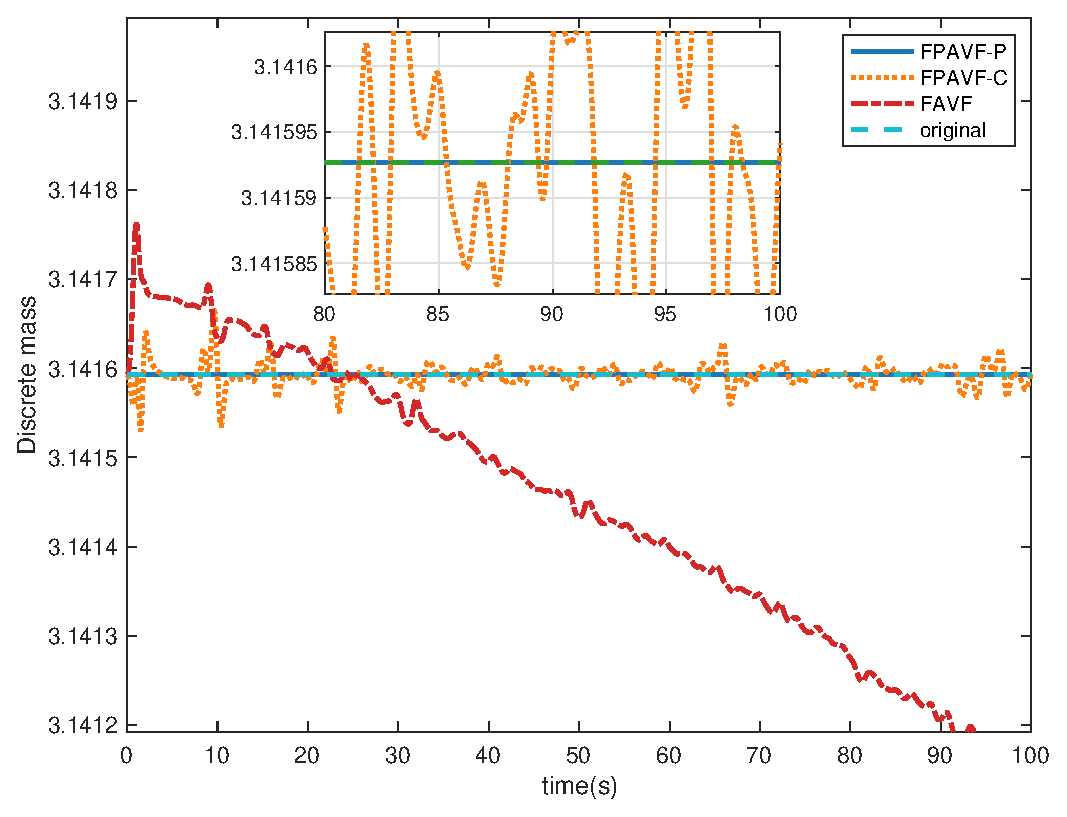
\includegraphics[width=0.3\textwidth]{./figure/exp2_M1.6.eps}
	%\centerline{($b$) $\alpha=1.6$}
	}\\
	 \subfigure[$\alpha=1.9$]{ \centering
	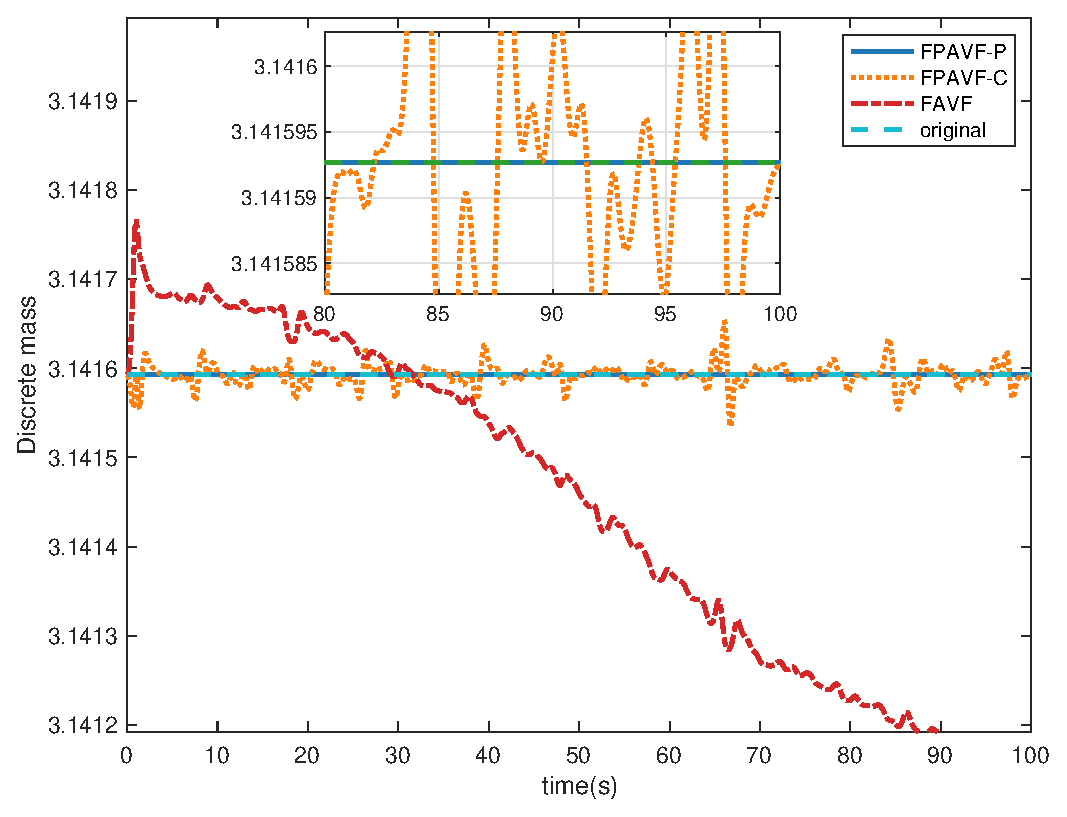
\includegraphics[width=0.3\textwidth]{./figure/exp2_M1.9.eps}
	%\centerline{($c$) $\alpha=1.9$}
	}\subfigure[$\alpha=2.0$]{ \centering
	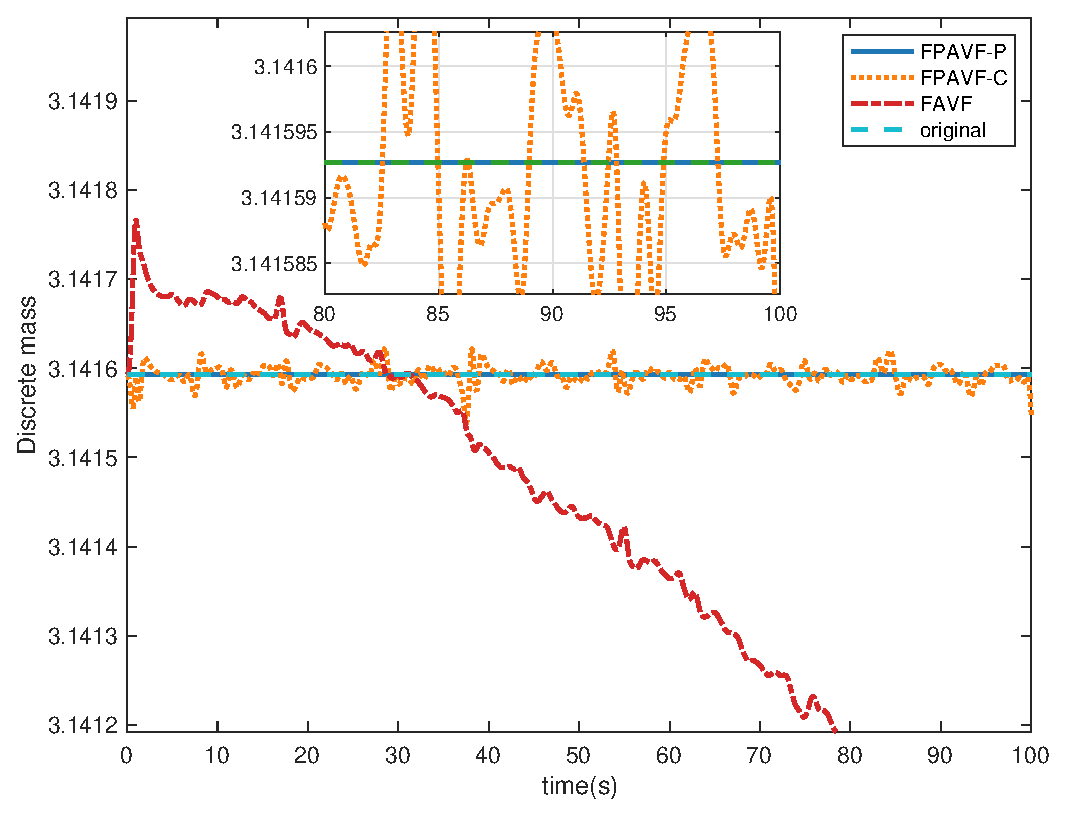
\includegraphics[width=0.3\textwidth]{./figure/exp2_M2.eps}
	%\centerline{($d$) $\alpha=2.0$}
	}
	% \caption{Discrete mass for different $\alpha$ in Example \ref{exp_PAVF:4} with $N = 64$ and $\tau=0.01$.} 
	\caption{当  $N = 64, \tau=0.01$ 时,算例 \ref{exp_PAVF:4}取不同 $\alpha$ 的离散质量.}
	\label{fig_PAVF:9}
	\end{center}
	\end{figure}

\begin{figure}[H]
	\begin{center}
	\subfigure[$\alpha=1.3$]{ \centering
	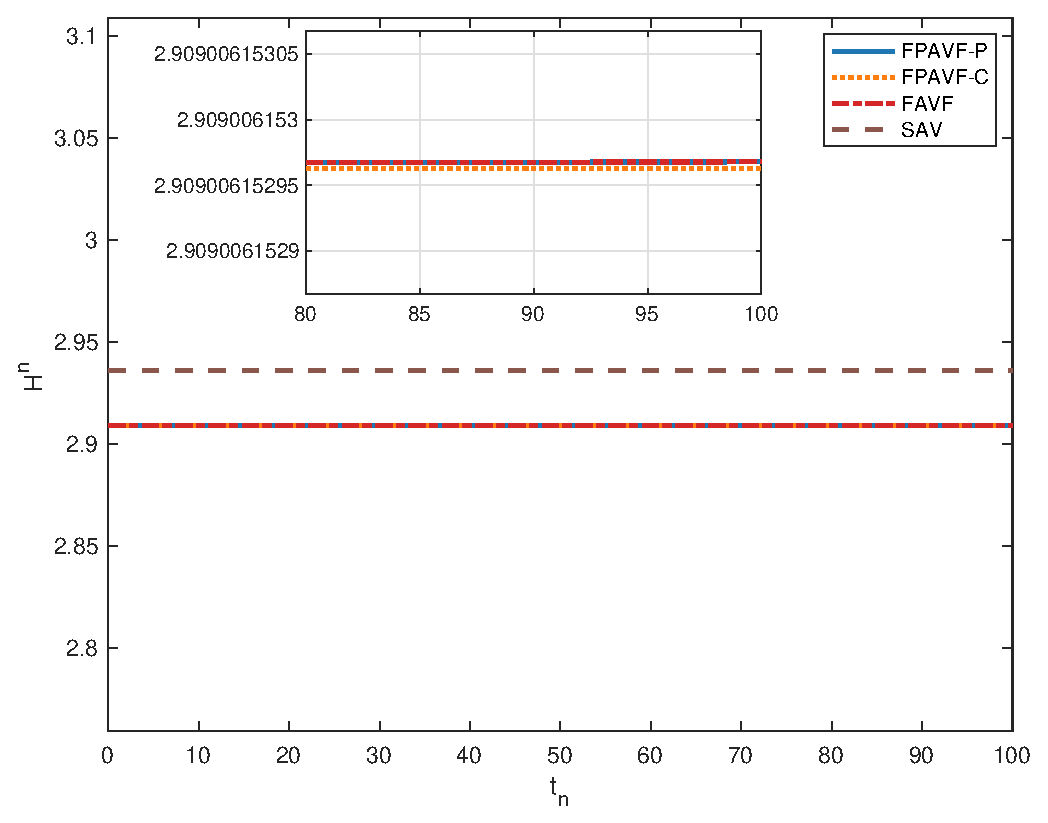
\includegraphics[width=0.3\textwidth]{./figure/exp2_H1.3.eps}
	%\centerline{($a$) $\alpha=1.3$}
	}\subfigure[$\alpha=1.6$]{ \centering
	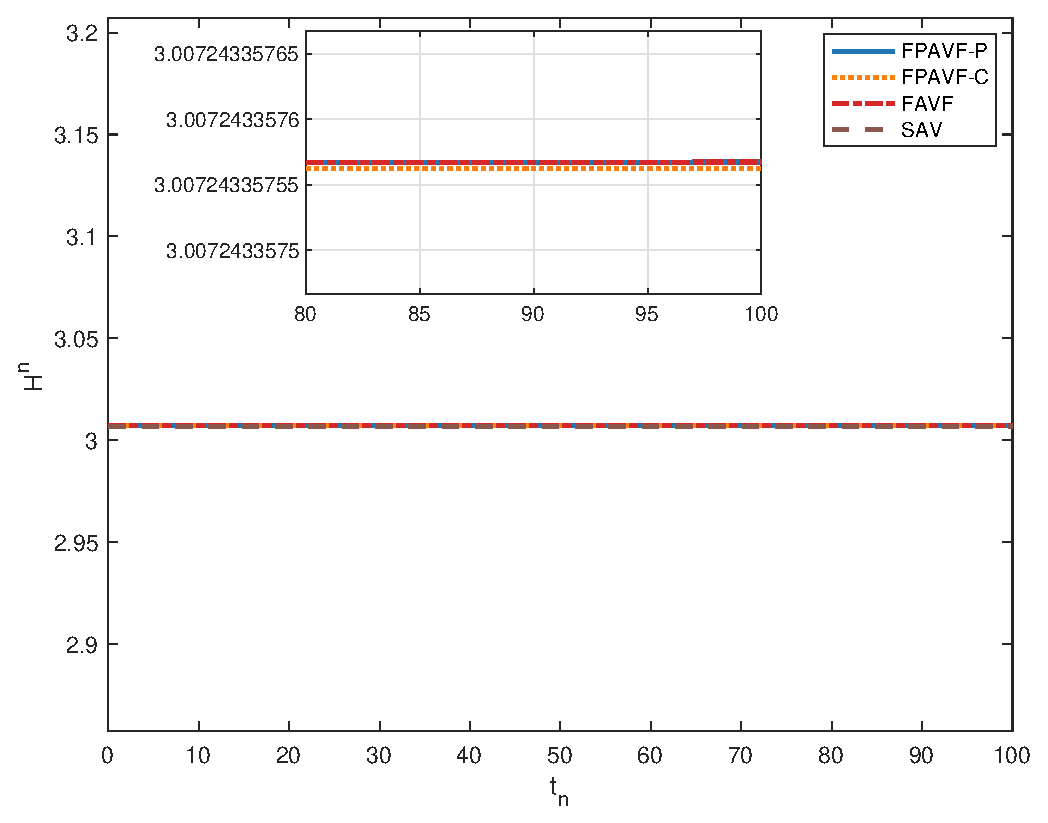
\includegraphics[width=0.3\textwidth]{./figure/exp2_H1.6.eps}
	%\centerline{($b$) $\alpha=1.6$}
	}\\
	\subfigure[$\alpha=1.9$]{ \centering
	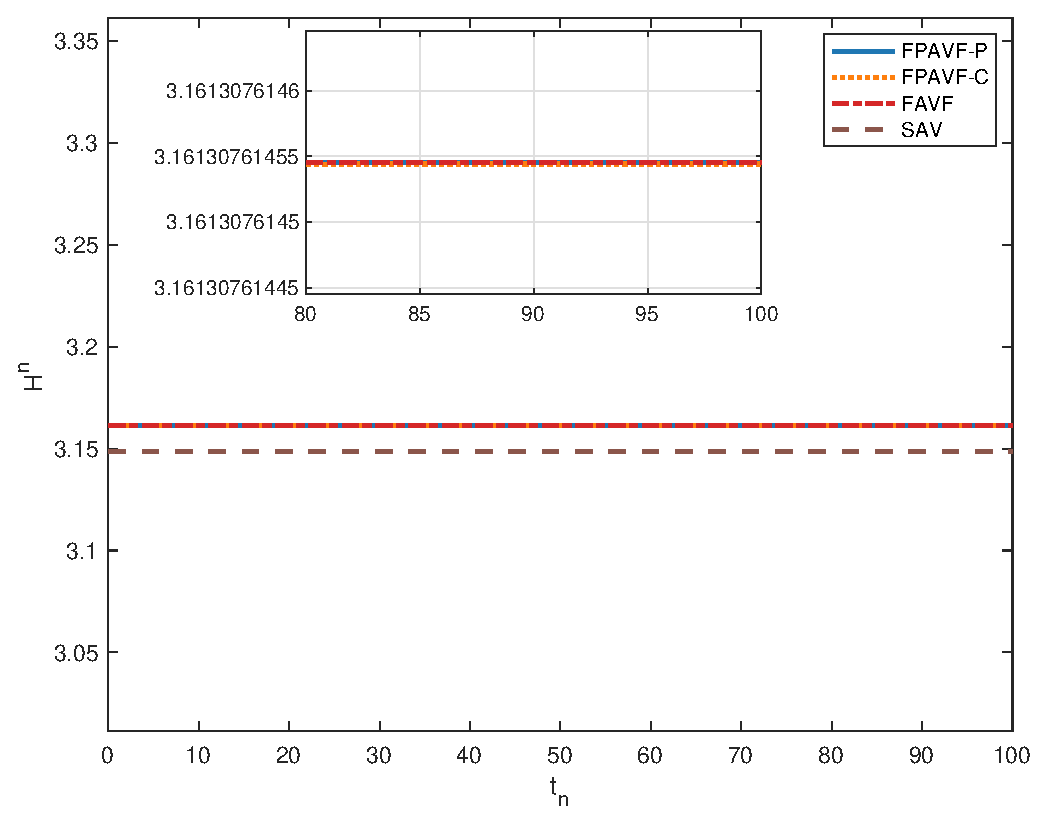
\includegraphics[width=0.3\textwidth]{./figure/exp2_H1.9.eps}
	%\centerline{($d$) $\alpha=2.0$}
	}\subfigure[$\alpha=2.0$]{ \centering
	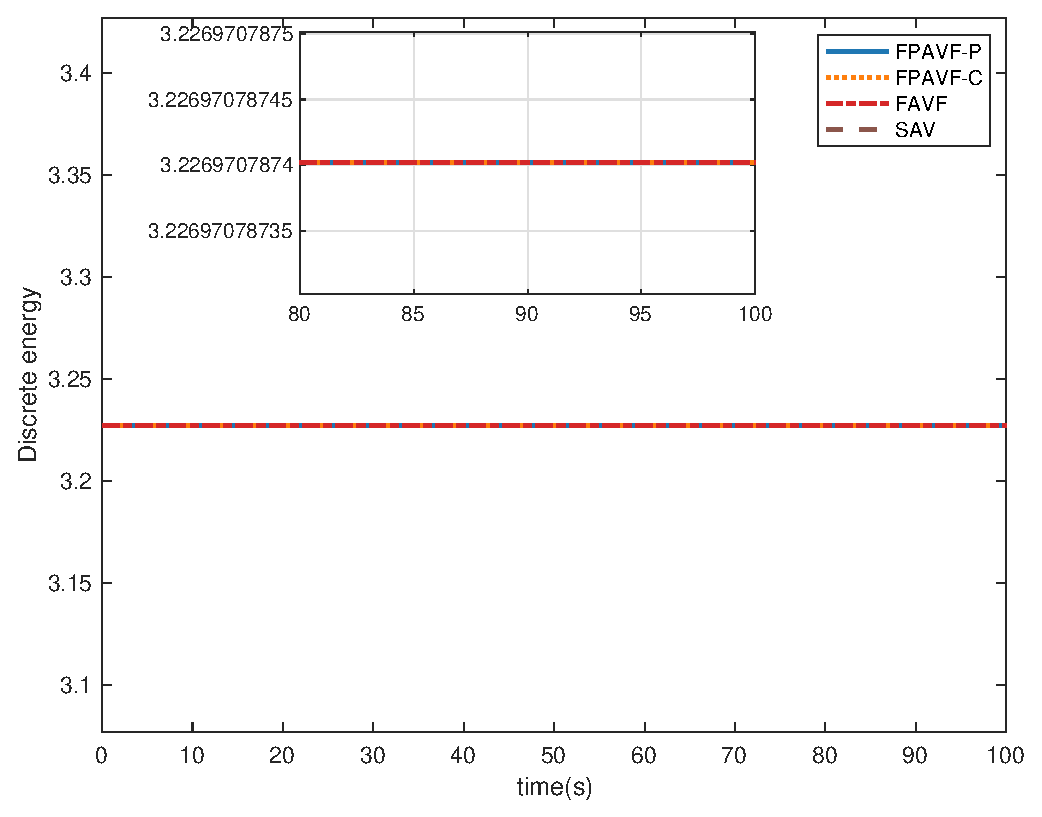
\includegraphics[width=0.3\textwidth]{./figure/exp2_H2.eps}
	%\centerline{($d$) $\alpha=2.0$}
	}
	% \caption{Discrete energy for different $\alpha$ in Example \ref{exp_PAVF:4} with $N = 64$ and $\tau=0.01$.} 
	\caption{当  $N = 64, \tau=0.01$ 时,算例 \ref{exp_PAVF:4}取不同 $\alpha$ 的离散能量.}
	\label{fig_PAVF:10}
	\end{center}
	\end{figure}
	与一维问题不同,二维情况下没有三层线性隐式格式, 因此只比较了 SAV 方法与本文提出的 FPAVF-P、FAVF 和 FPAVF-C 格式的性能.
	图 \ref{fig_PAVF:9} - \ref{fig_PAVF:10} 展示了在不同 $\alpha$ 下通过 $N=64$ 和 $\tau=0.01$ 计算的离散质量和离散能量的演变(T=100).
	图 \ref{fig_PAVF:11} - \ref{fig_PAVF:12} 展示了随时间变化的离散质量和能量相对误差的变化.
	可以观察到,FPAVF-P 格式在原始质量上收敛得很好,其他三种方法性能较差,尤其是 FAVF 格式和 FPAVF 格式(FPAVF格式的结果未显示,因为它更为糟糕).
	本章提出的三种格式都能很好地保持原始能量,而 SAV 方法只能保持一个修正的能量.
	这些现象再次验证了理论结果的正确性.
\begin{figure}[H]
\begin{center}
 \subfigure[$\alpha=1.3$]{ \centering
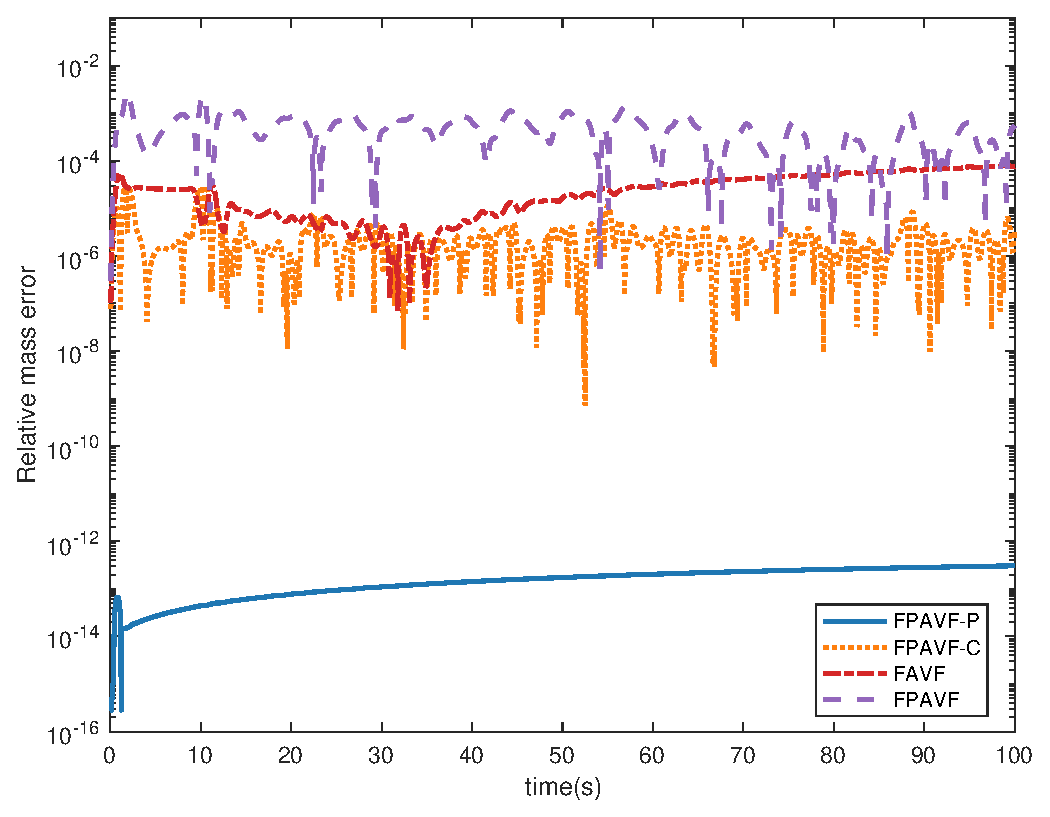
\includegraphics[width=0.3\textwidth]{./figure/exp2_RM1.3.eps}
%\centerline{($a$) $\alpha=1.3$}
}\subfigure[$\alpha=1.6$]{ \centering
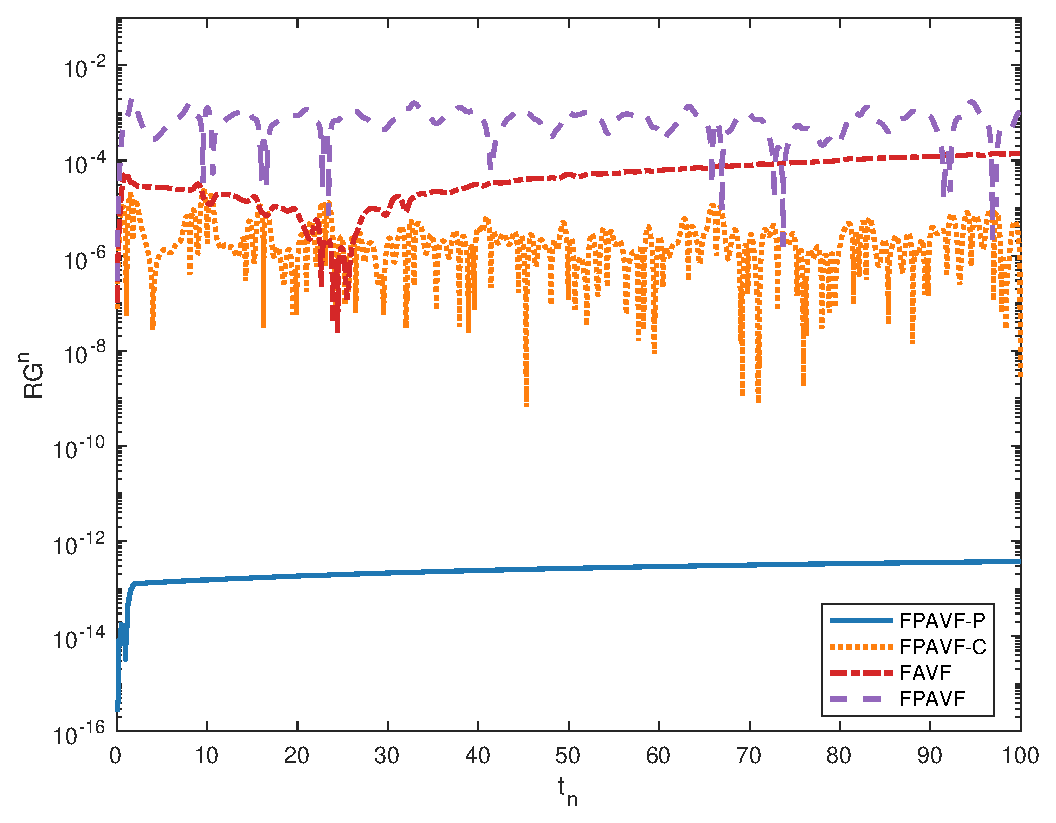
\includegraphics[width=0.3\textwidth]{./figure/exp2_RM1.6.eps}
%\centerline{($b$) $\alpha=1.6$}
}\subfigure[$\alpha=1.9$]{ \centering
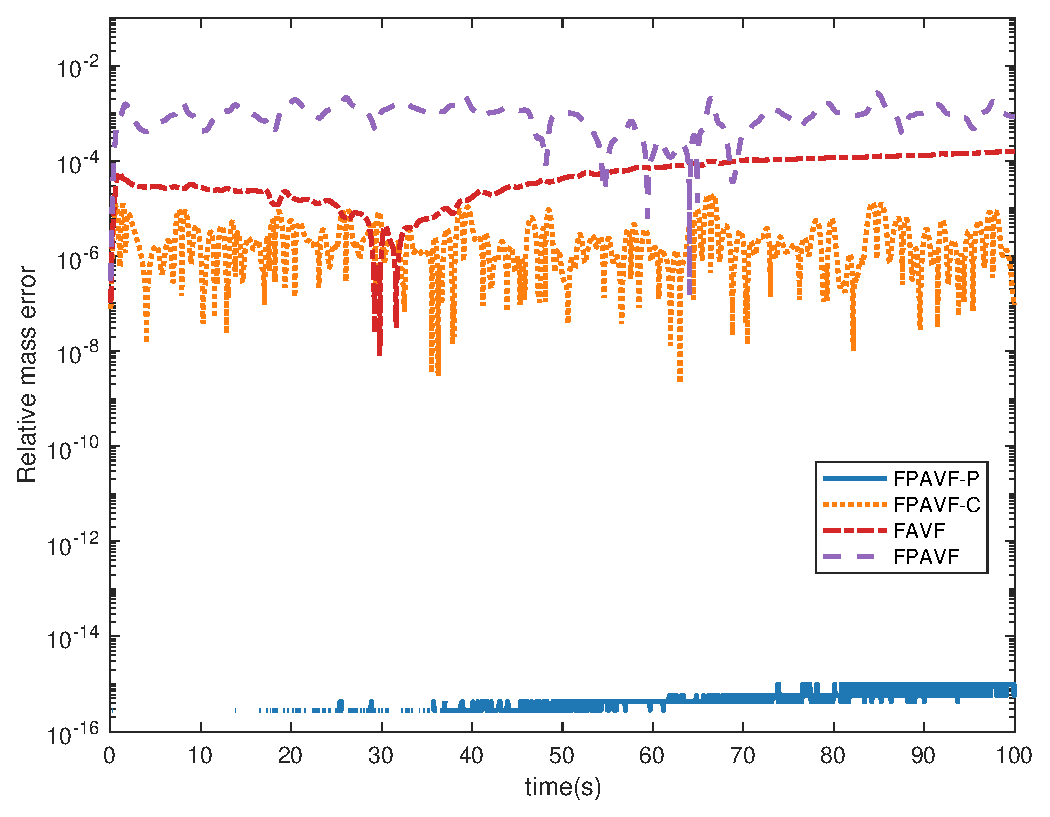
\includegraphics[width=0.3\textwidth]{./figure/exp2_RM1.9.eps}
%\centerline{($c$) $\alpha=1.9$}
}
% \caption{The relative errors of discrete mass for different $\alpha$ in Example \ref{exp_PAVF:4} with $N = 64$ and $\tau=0.01$.} 
\caption{当  $N = 64, \tau=0.01$ 时,算例 \ref{exp_PAVF:4}取不同 $\alpha$ 的相对质量误差}
\label{fig_PAVF:11}
\end{center}
\end{figure}


\begin{figure}[H]
\begin{center}
 \subfigure[$\alpha=1.3$]{ \centering
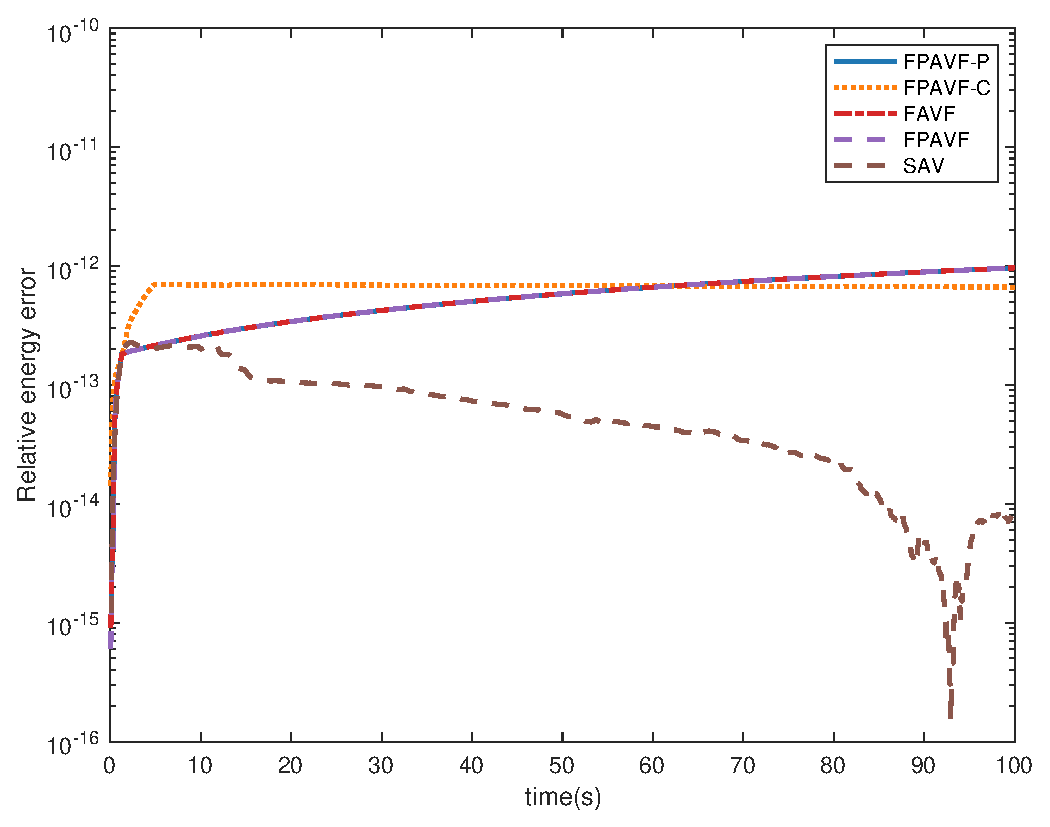
\includegraphics[width=0.3\textwidth]{./figure/exp2_RH1.3.eps}
%\centerline{($a$) $\alpha=1.3$}
}\subfigure[$\alpha=1.6$]{ \centering
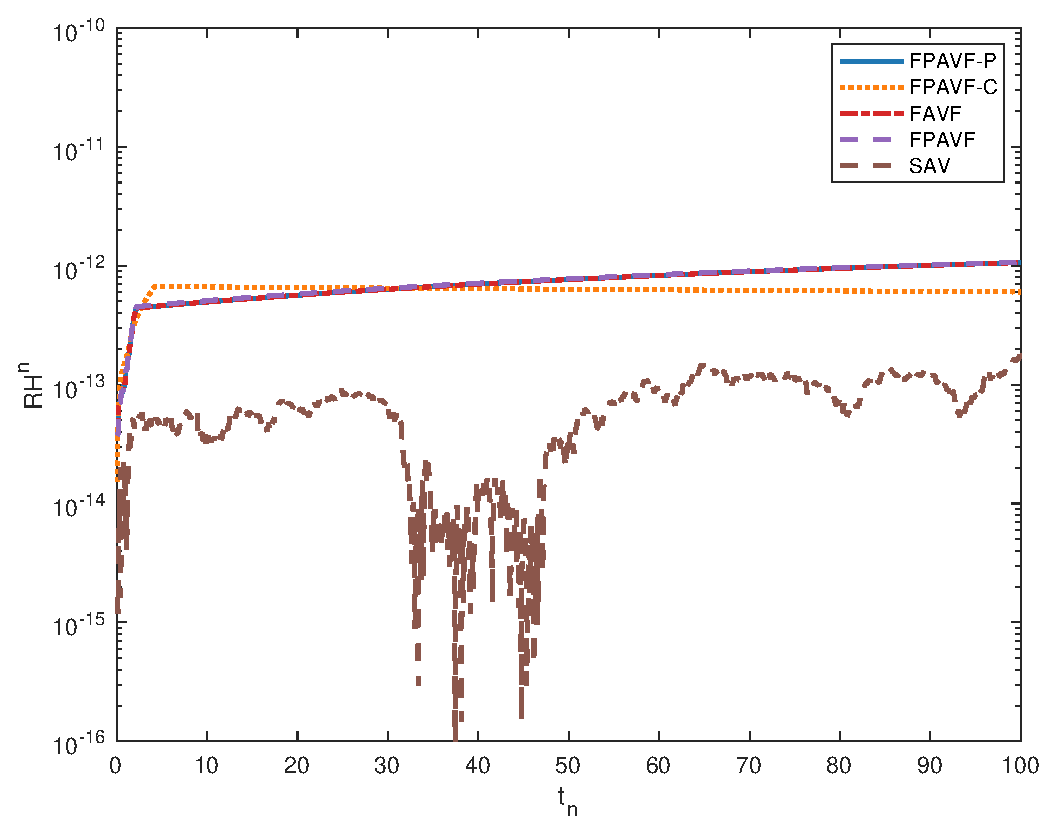
\includegraphics[width=0.3\textwidth]{./figure/exp2_RH1.6.eps}
%\centerline{($b$) $\alpha=1.6$}
} \subfigure[$\alpha=1.9$]{ \centering
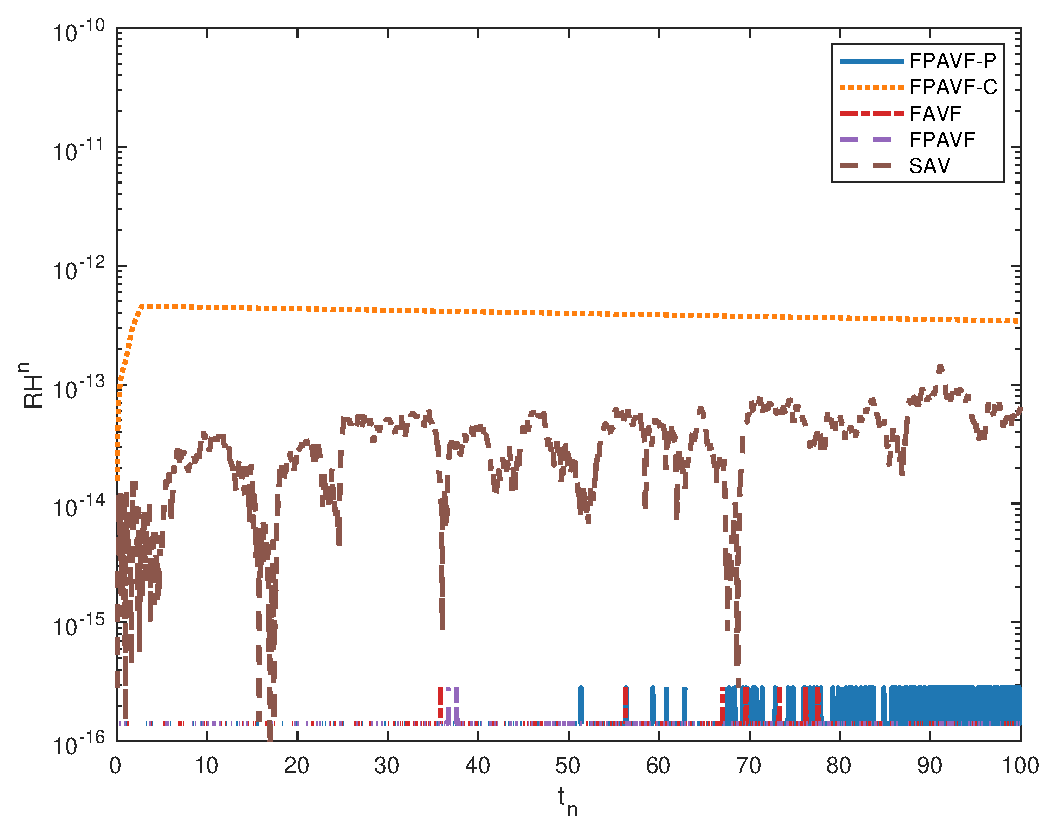
\includegraphics[width=0.3\textwidth]{./figure/exp2_RH1.9.eps}
%\centerline{($c$) $\alpha=1.9$}
}
% \caption{The relative errors of discrete energy for different $\alpha$ in Example \ref{exp_PAVF:4} with $N = 64$ and $\tau=0.01$.} 
\caption{当  $N = 64, \tau=0.01$ 时,算例 \ref{exp_PAVF:4}取不同 $\alpha$ 的相对能量误差}
\label{fig_PAVF:12}
\end{center}
\end{figure}

更详细的比较结果见表 \ref{tab_PAVF:4-1} - \ref{tab_PAVF:4-4},观察这些数据,可得到同样的结论.

\begin{table}[H]\footnotesize
	\centering
	% \caption{Discrete energy $H^{m}$ at time $t=t_{m}$ for Example \ref{exp_PAVF:4} when $\alpha=2$.}
	\caption{当 $\alpha=2.0$ 时,算例 \ref{exp_PAVF:4} 在时刻 $t=t_{m}$ 的离散能量 $H^{m}$.}
	\begin{tabular}{llllll}
	  \toprule
       $t$   &FAVF   &FPAVF   &FPAVF-C   &SAV   &FPAVF-P\\
	%   \midrule
	%   0     & 3.22697078740176 & 3.22697078740176 & 3.22697078740173 & 3.21234862767094 & 3.22697078740176 \\
	%   10    & 3.22697078740176 & 3.22697078740176 & 3.22697078740168 & 3.21234862767062 & 3.22697078740176 \\
	%   20    & 3.22697078740176 & 3.22697078740176 & 3.22697078740172 & 3.21234862767066 & 3.22697078740176 \\
	%   40    & 3.22697078740175 & 3.22697078740176 & 3.22697078740182 & 3.21234862767033 & 3.22697078740176 \\
	%   60    & 3.22697078740176 & 3.22697078740176 & 3.22697078740191 & 3.21234862767035 & 3.22697078740176 \\
	%   80    & 3.22697078740176 & 3.22697078740175 & 3.22697078740199 & 3.21234862767073 & 3.22697078740176 \\
	%   100   & 3.22697078740175 & 3.22697078740176 & 3.22697078740207 & 3.21234862767045 & 3.22697078740176 \\
	%   \midrule
	\midrule
	0     & \textcolor{purple}{3.22697078}740176 & \textcolor{purple}{3.22697078}740176 & \textcolor{purple}{3.22697078}740173 & \textcolor{purple}{3.2}1234862767094 & \textcolor{purple}{3.22697078}740176 \\
	10    & \textcolor{purple}{3.22697078}740176 & \textcolor{purple}{3.22697078}740176 & \textcolor{purple}{3.22697078}740168 & \textcolor{purple}{3.2}1234862767062 & \textcolor{purple}{3.22697078}740176 \\
	20    & \textcolor{purple}{3.22697078}740176 & \textcolor{purple}{3.22697078}740176 & \textcolor{purple}{3.22697078}740172 & \textcolor{purple}{3.2}1234862767066 & \textcolor{purple}{3.22697078}740176 \\
	40    & \textcolor{purple}{3.22697078}740175 & \textcolor{purple}{3.22697078}740176 & \textcolor{purple}{3.22697078}740182 & \textcolor{purple}{3.2}1234862767033 & \textcolor{purple}{3.22697078}740176 \\
	60    & \textcolor{purple}{3.22697078}740176 & \textcolor{purple}{3.22697078}740176 & \textcolor{purple}{3.22697078}740191 & \textcolor{purple}{3.2}1234862767035 & \textcolor{purple}{3.22697078}740176 \\
	80    & \textcolor{purple}{3.22697078}740176 & \textcolor{purple}{3.22697078}740175 & \textcolor{purple}{3.22697078}740199 & \textcolor{purple}{3.2}1234862767073 & \textcolor{purple}{3.22697078}740176 \\
	100   & \textcolor{purple}{3.22697078}740175 & \textcolor{purple}{3.22697078}740176 & \textcolor{purple}{3.22697078}740207 & \textcolor{purple}{3.2}1234862767045 & \textcolor{purple}{3.22697078}740176 \\
	\midrule
	  \multicolumn{6}{r}{Original energy:~3.22697078976648} \\
	  \bottomrule
	  \end{tabular}\label{tab_PAVF:4-1}%
  \end{table}%


  % Table generated by Excel2LaTeX from sheet 'Sheet1'
\begin{table}[H]\footnotesize
	\centering
	% \caption{Discrete mass $G^{m}$ at time $t=t_{m}$ for Example \ref{exp_PAVF:4} when $\alpha=1.3$.}
	\caption{当 $\alpha=1.3$ 时,算例 \ref{exp_PAVF:4} 在时刻 $t=t_{m}$ 的离散质量 $G^{m}$.}
	  \begin{tabular}{lllll}
	  \toprule
$t$   &FAVF   &FPAVF   &FPAVF-C   &FPAVF-P\\
	%   \midrule
	%   0     & 3.14159297667455 & 3.14159361842152 & 3.14159241227909 & 3.14159265358976 \\
	%   10    & 3.14160952253933 & 3.13595374862870 & 3.14166505643569 & 3.14159265358963 \\
	%   20    & 3.14161343543099 & 3.14421089321261 & 3.14158965037808 & 3.14159265358952 \\
	%   40    & 3.14157539023564 & 3.14362067013654 & 3.14159917106759 & 3.14159265358932 \\
	%   60    & 3.14150249358846 & 3.14217508702013 & 3.14159868539556 & 3.14159265358912 \\
	%   80    & 3.14143174175214 & 3.14159826267015 & 3.14158946625201 & 3.14159265358895 \\
	%   100   & 3.14135672071641 & 3.14328710863969 & 3.14158227319751 & 3.14159265358880 \\
	%   \midrule
	\midrule
	0     & \textcolor{purple}{3.141592}97667455 & \textcolor{purple}{3.14159}361842152 & \textcolor{purple}{3.141592}41227909 & \textcolor{purple}{3.141592653}58976 \\
	10    & \textcolor{purple}{3.141}60952253933 & \textcolor{purple}{3.1}3595374862870 & \textcolor{purple}{3.141}66505643569 & \textcolor{purple}{3.141592653}58963 \\
	20    & \textcolor{purple}{3.141}61343543099 & \textcolor{purple}{3.14}421089321261 & \textcolor{purple}{3.1415}8965037808 & \textcolor{purple}{3.141592653}58952 \\
	40    & \textcolor{purple}{3.1415}7539023564 & \textcolor{purple}{3.14}362067013654 & \textcolor{purple}{3.14159}917106759 & \textcolor{purple}{3.141592653}58932 \\
	60    & \textcolor{purple}{3.1415}0249358846 & \textcolor{purple}{3.14}217508702013 & \textcolor{purple}{3.14159}868539556 & \textcolor{purple}{3.141592653}58912 \\
	80    & \textcolor{purple}{3.141}43174175214 & \textcolor{purple}{3.14159}826267015 & \textcolor{purple}{3.1415}8946625201 & \textcolor{purple}{3.141592653}58895 \\
	100   & \textcolor{purple}{3.141}35672071641 & \textcolor{purple}{3.14}328710863969 & \textcolor{purple}{3.1415}8227319751 & \textcolor{purple}{3.141592653}58880 \\
	\midrule
	  \multicolumn{5}{r}{Original mass:~3.14159265323701} \\
	  \bottomrule
	  \end{tabular}\label{tab_PAVF:4-2}%
  \end{table}%

  % Table generated by Excel2LaTeX from sheet 'Sheet1'
\begin{table}[H]\footnotesize
	\centering
	% \caption{Discrete mass $G^{m}$ at time $t=t_{m}$ for Example \ref{exp_PAVF:4} when $\alpha=1.6$.}
	\caption{当 $\alpha=1.6$ 时,算例 \ref{exp_PAVF:4} 在时刻 $t=t_{m}$ 的离散质量 $G^{m}$.}
	 \begin{tabular}{lllll}
	  \toprule
$t$   &FAVF   &FPAVF   &FPAVF-C   &FPAVF-P\\
	%   \midrule
	%   0     & 3.14159297668940 & 3.14159361814729 & 3.14159241218683 & 3.14159265358976 \\
	%   10    & 3.14163389358031 & 3.13754191888209 & 3.14160072631792 & 3.14159265358928 \\
	%   20    & 3.14161716177523 & 3.14433222488425 & 3.14159044899067 & 3.14159265358919 \\
	%   40    & 3.14149554093894 & 3.14475213344308 & 3.14160500647197 & 3.14159265358901 \\
	%   60    & 3.14139997924855 & 3.14288256207779 & 3.14160023436812 & 3.14159265358885 \\
	%   80    & 3.14127488637752 & 3.14241392600216 & 3.14158768432513 & 3.14159265358871 \\
	%   100   & 3.14115287766347 & 3.14489331385338 & 3.14159412822417 & 3.14159265358860 \\
	% 	\midrule
	\midrule
	0     & \textcolor{purple}{3.141592}97668940 & \textcolor{purple}{3.14159}361814729 & \textcolor{purple}{3.141592}41218683 & \textcolor{purple}{3.141592653}58976 \\
	10    & \textcolor{purple}{3.141}63389358031 & \textcolor{purple}{3.13}754191888209 & \textcolor{purple}{3.141}60072631792 & \textcolor{purple}{3.141592653}58928 \\
	20    & \textcolor{purple}{3.141}61716177523 & \textcolor{purple}{3.14}433222488425 & \textcolor{purple}{3.14159}044899067 & \textcolor{purple}{3.141592653}58919 \\
	40    & \textcolor{purple}{3.141}49554093894 & \textcolor{purple}{3.14}475213344308 & \textcolor{purple}{3.141}60500647197 & \textcolor{purple}{3.141592653}58901 \\
	60    & \textcolor{purple}{3.141}39997924855 & \textcolor{purple}{3.14}288256207779 & \textcolor{purple}{3.141}60023436812 & \textcolor{purple}{3.141592653}58885 \\
	80    & \textcolor{purple}{3.141}27488637752 & \textcolor{purple}{3.14}241392600216 & \textcolor{purple}{3.1415}8768432513 & \textcolor{purple}{3.141592653}58871 \\
	100   & \textcolor{purple}{3.141}15287766347 & \textcolor{purple}{3.14}489331385338 & \textcolor{purple}{3.14159}412822417 & \textcolor{purple}{3.141592653}58860 \\
	  \midrule
	  \multicolumn{5}{r}{Original mass:~3.14159265323701} \\
	  \bottomrule
	  \end{tabular}\label{tab_PAVF:4-3}%
  \end{table}%

  % Table generated by Excel2LaTeX from sheet 'Sheet1'
\begin{table}[H]\footnotesize
	\centering
	% \caption{Discrete mass $G^{m}$ at time $t=t_{m}$ for Example \ref{exp_PAVF:4} when $\alpha=2$.}
	\caption{当 $\alpha=2.0$ 时,算例 \ref{exp_PAVF:4} 在时刻 $t=t_{m}$ 的离散质量 $G^{m}$.}
	\begin{tabular}{lllll}
	  \toprule
$t$   &FAVF   &FPAVF   &FPAVF-C   &FPAVF-P\\
	%   \midrule
	%   0     & 3.14159297725470 & 3.14159361919902 & 3.14159241149324 & 3.14159265358976 \\
	%   10    & 3.14168000260412 & 3.14369215006721 & 3.14160070161208 & 3.14159265358976 \\
	%   20    & 3.14164544531849 & 3.14521250122401 & 3.14158745249453 & 3.14159265358976 \\
	%   40    & 3.14150535695500 & 3.14531702832209 & 3.14160031804829 & 3.14159265358976 \\
	%   60    & 3.14136438511727 & 3.14552013864766 & 3.14159560564481 & 3.14159265358976 \\
	%   80    & 3.14118013227991 & 3.14739329967543 & 3.14158800109644 & 3.14159265358976 \\
	%   100   & 3.14101125059928 & 3.15011874273391 & 3.14154787019595 & 3.14159265358976 \\
	%   \midrule
	\midrule
	0     & \textcolor{purple}{3.141592}97725470 & \textcolor{purple}{3.14159}361919902 & \textcolor{purple}{3.141592}41149324 & \textcolor{purple}{3.141592653}58976 \\
	10    & \textcolor{purple}{3.141}68000260412 & \textcolor{purple}{3.14}369215006721 & \textcolor{purple}{3.141}60070161208 & \textcolor{purple}{3.141592653}58976 \\
	20    & \textcolor{purple}{3.141}64544531849 & \textcolor{purple}{3.14}521250122401 & \textcolor{purple}{3.1415}8745249453 & \textcolor{purple}{3.141592653}58976 \\
	40    & \textcolor{purple}{3.1415}0535695500 & \textcolor{purple}{3.14}531702832209 & \textcolor{purple}{3.141}60031804829 & \textcolor{purple}{3.141592653}58976 \\
	60    & \textcolor{purple}{3.141}36438511727 & \textcolor{purple}{3.14}552013864766 & \textcolor{purple}{3.14159}560564481 & \textcolor{purple}{3.141592653}58976 \\
	80    & \textcolor{purple}{3.141}18013227991 & \textcolor{purple}{3.14}739329967543 & \textcolor{purple}{3.1415}8800109644 & \textcolor{purple}{3.141592653}58976 \\
	100   & \textcolor{purple}{3.141}01125059928 & \textcolor{purple}{3.1}5011874273391 & \textcolor{purple}{3.1415}4787019595 & \textcolor{purple}{3.141592653}58976 \\
	\midrule
	  \multicolumn{5}{r}{Original mass:~3.14159265323701} \\
	  \bottomrule
	  \end{tabular}\label{tab_PAVF:4-4}%
  \end{table}%

  最后,分别在图 \ref{fig_PAVF:13}-\ref{fig_PAVF:16} 中展示了 $\alpha=1.3,1.6,1.99,2$ 时波的演化过程(取$N=128$ 、 $\tau=0.01$).
  可以观察到,阶数 $\alpha$ 将显著影响波的形状,当 $\alpha$ 变大时,波的形状变化更快.特别地,当 $\alpha \rightarrow 2$ 时,数值解收敛到经典的非线性薛定谔波动方程 \cite{zhangConservativeNumericalScheme2003,liCompactFiniteDifference2012,wangAnalysisNewConservative2006}.

  \begin{figure}[H]
	\begin{center}
	 \subfigure[$t=0s$]{ \centering
	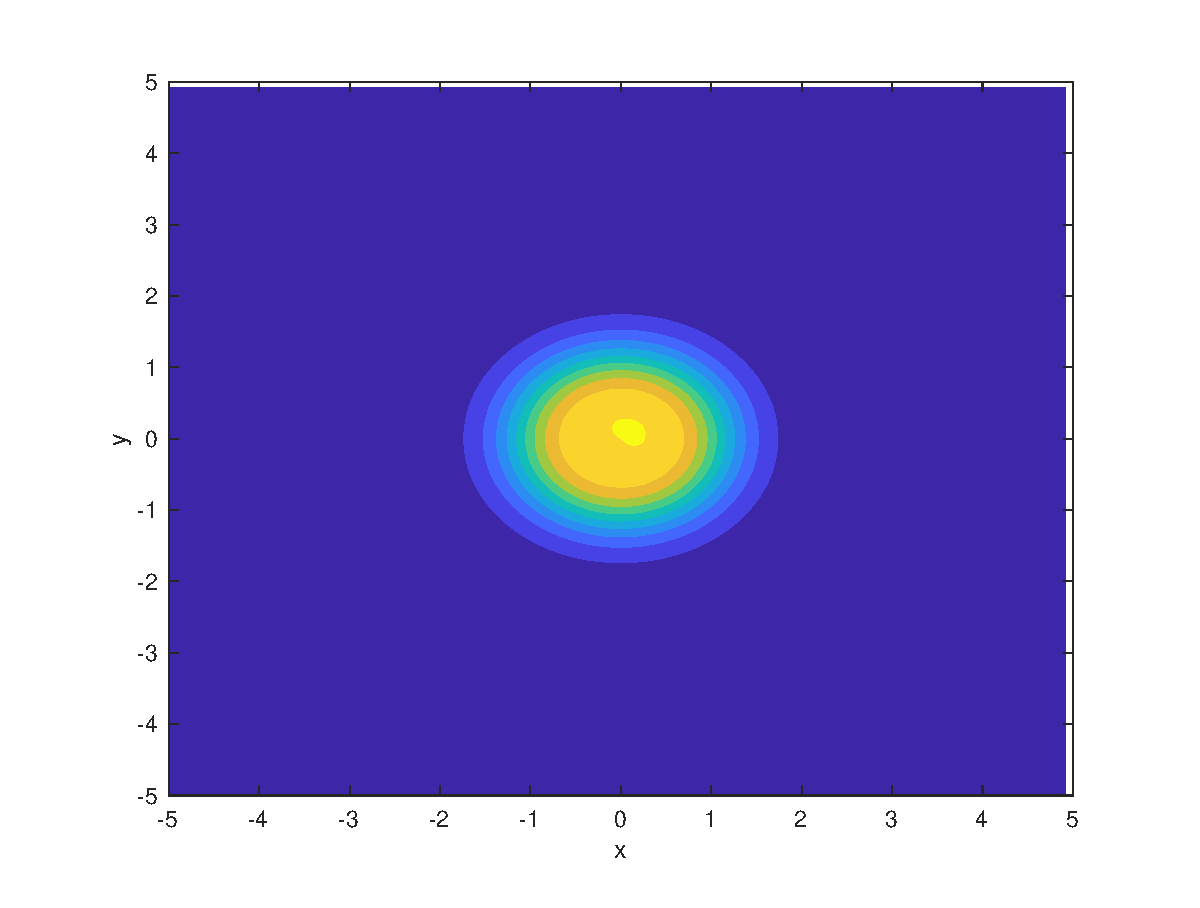
\includegraphics[width=0.3\textwidth]{./figure/exp2_contour3_p0.eps}
	}\subfigure[$t=1s$]{ \centering
	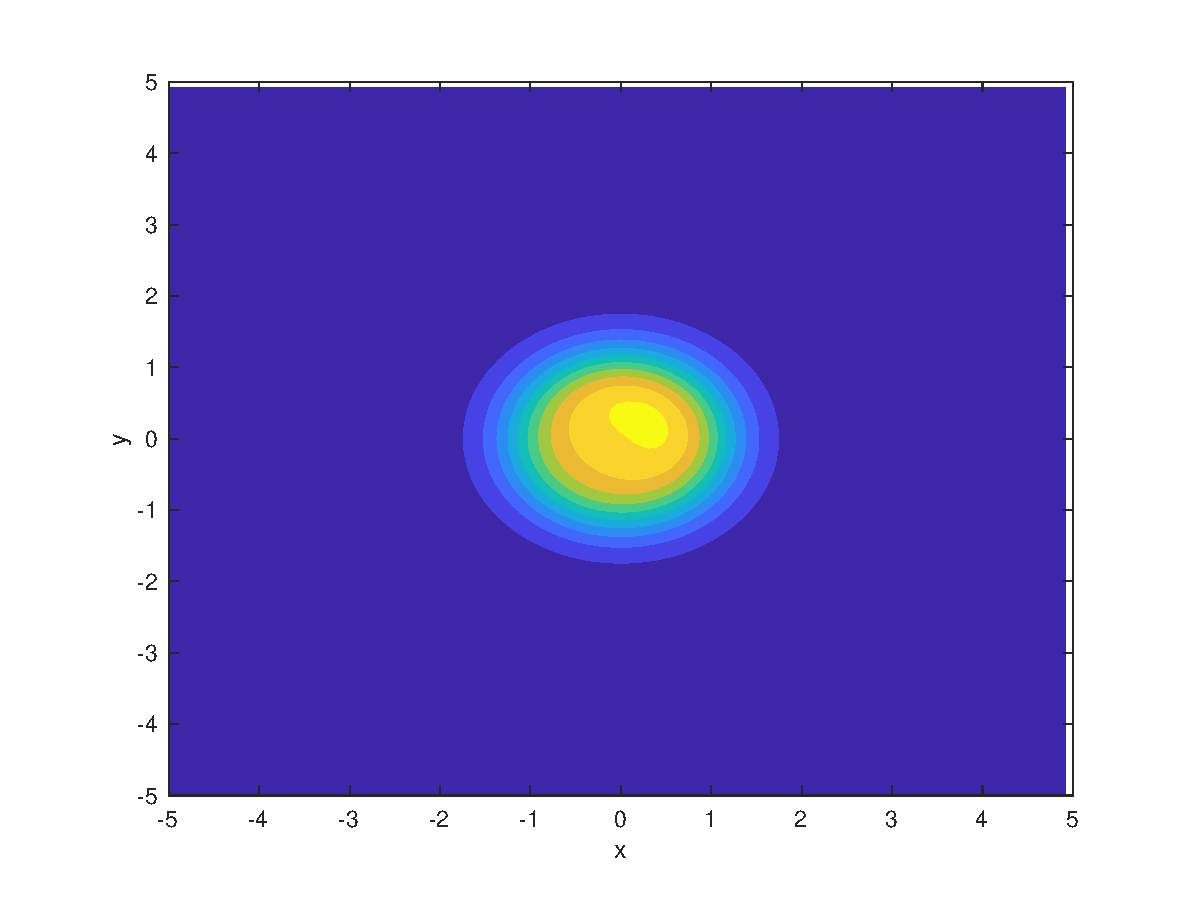
\includegraphics[width=0.3\textwidth]{./figure/exp2_contour3_p1.eps}
	} \subfigure[$t=5s$]{ \centering
	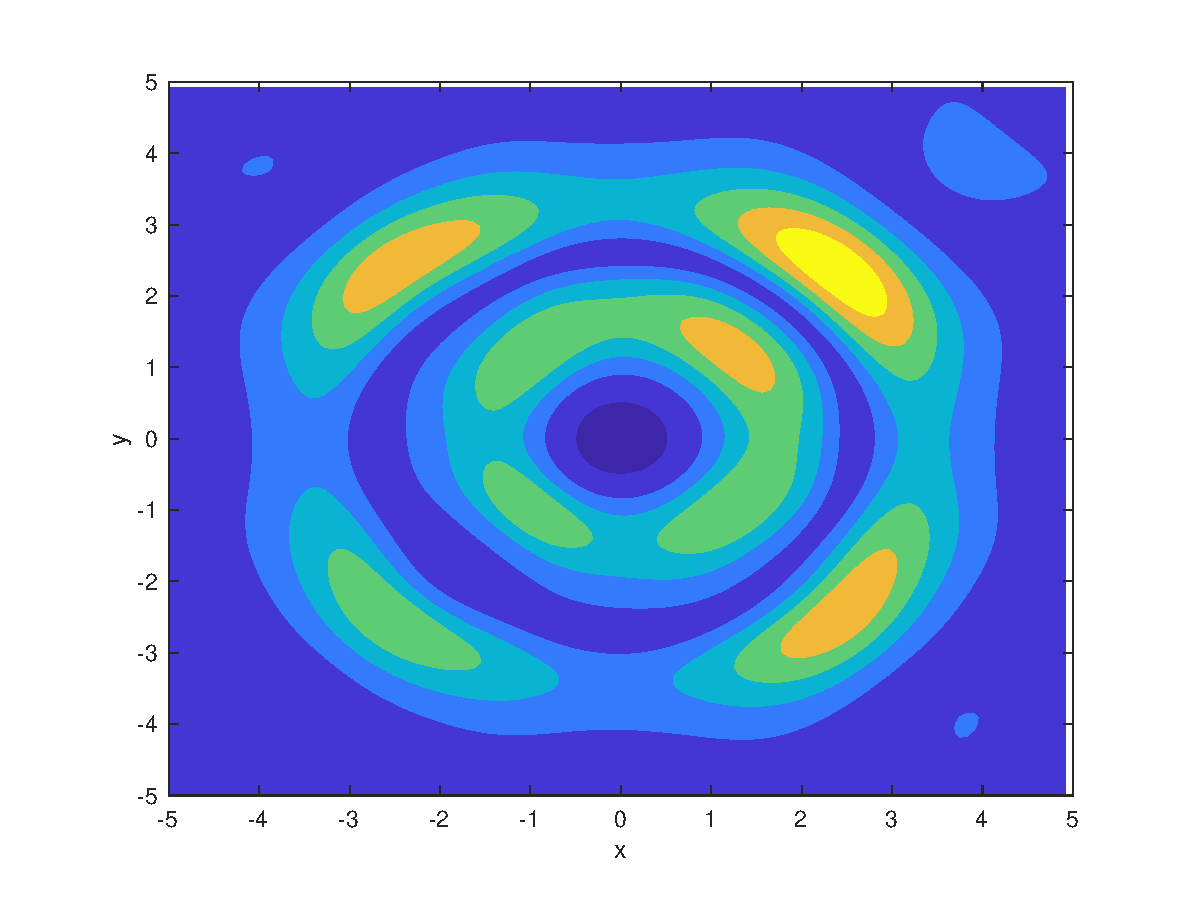
\includegraphics[width=0.3\textwidth]{./figure/exp2_contour3_p5.eps}
	}\\
	\subfigure[$t=10s$]{ \centering
	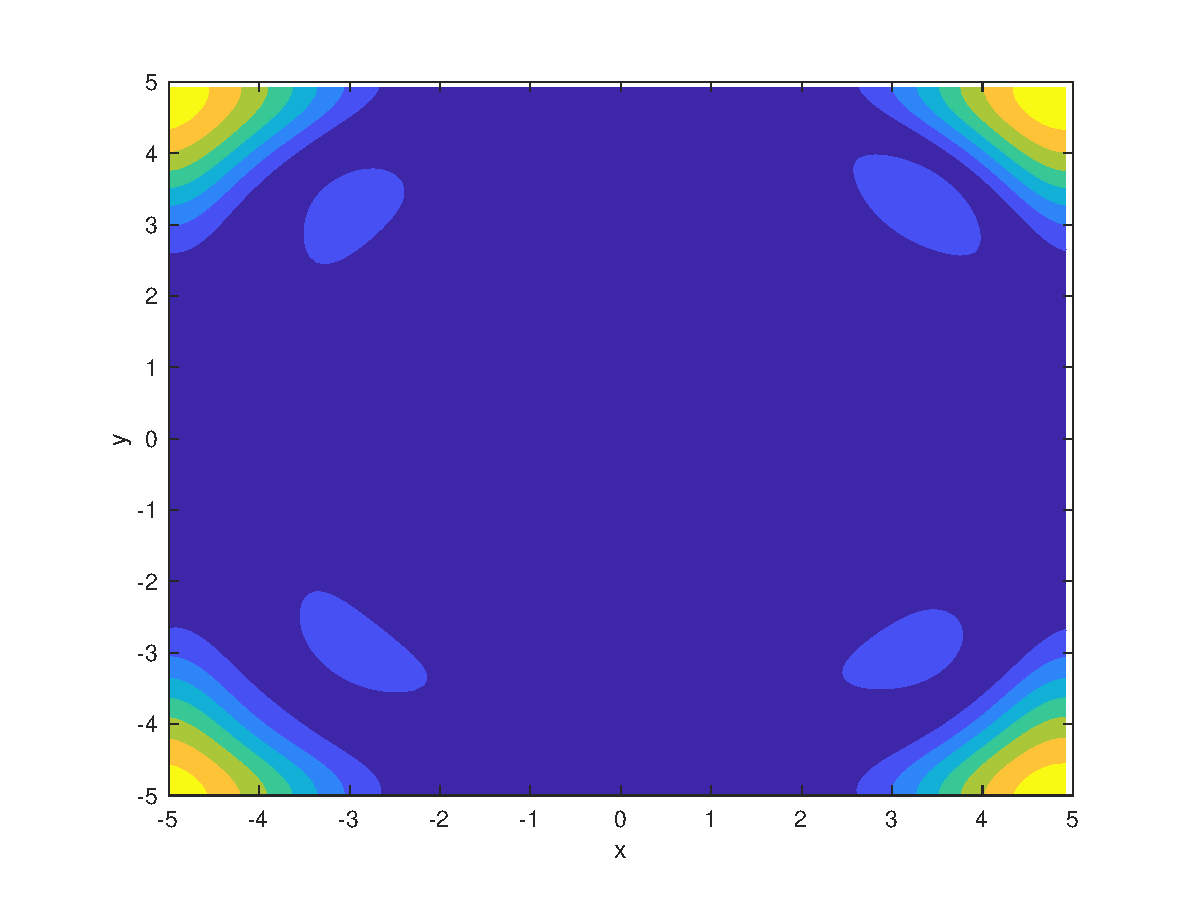
\includegraphics[width=0.3\textwidth]{./figure/exp2_contour3_p10.eps}
	}\subfigure[$t=50s$]{ \centering
	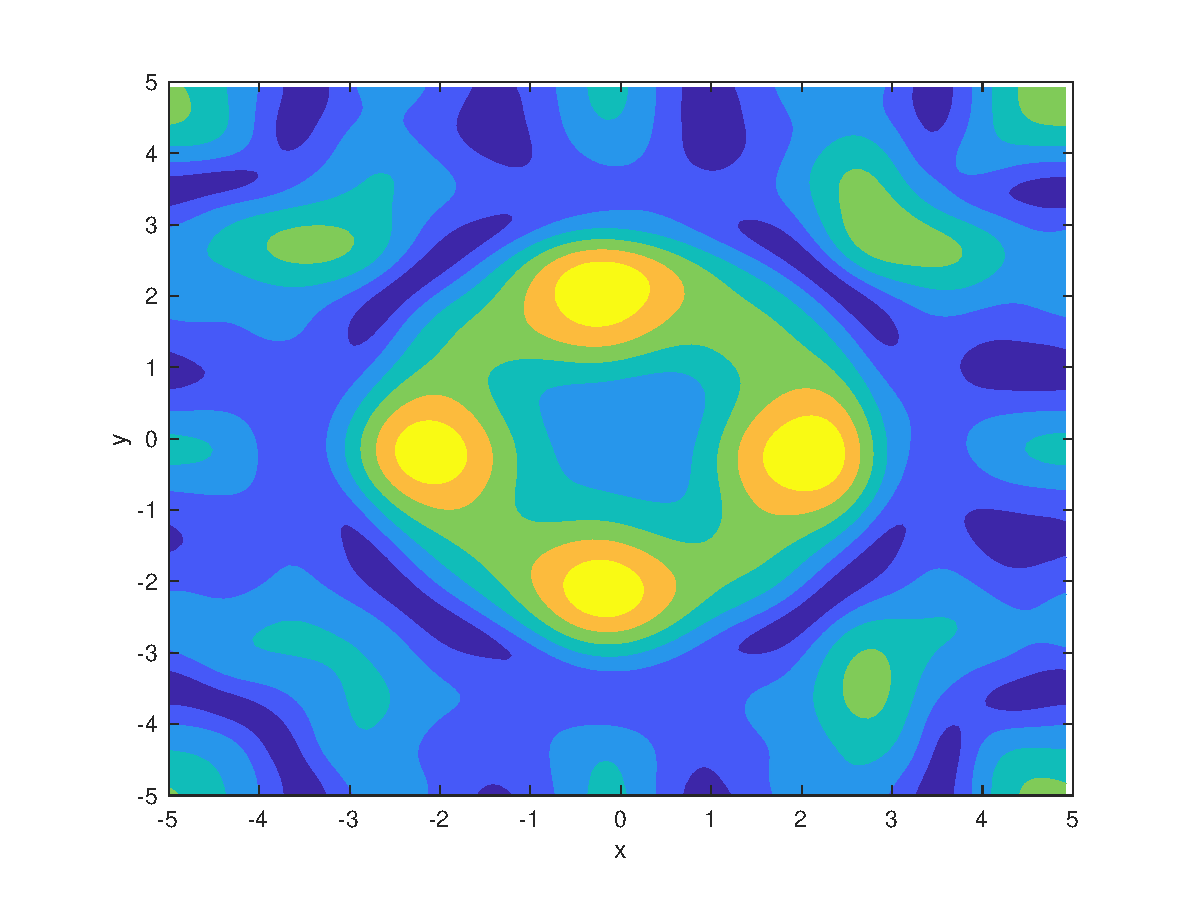
\includegraphics[width=0.3\textwidth]{./figure/exp2_contour3_p50.eps}
	} \subfigure[$t=100s$]{ \centering
	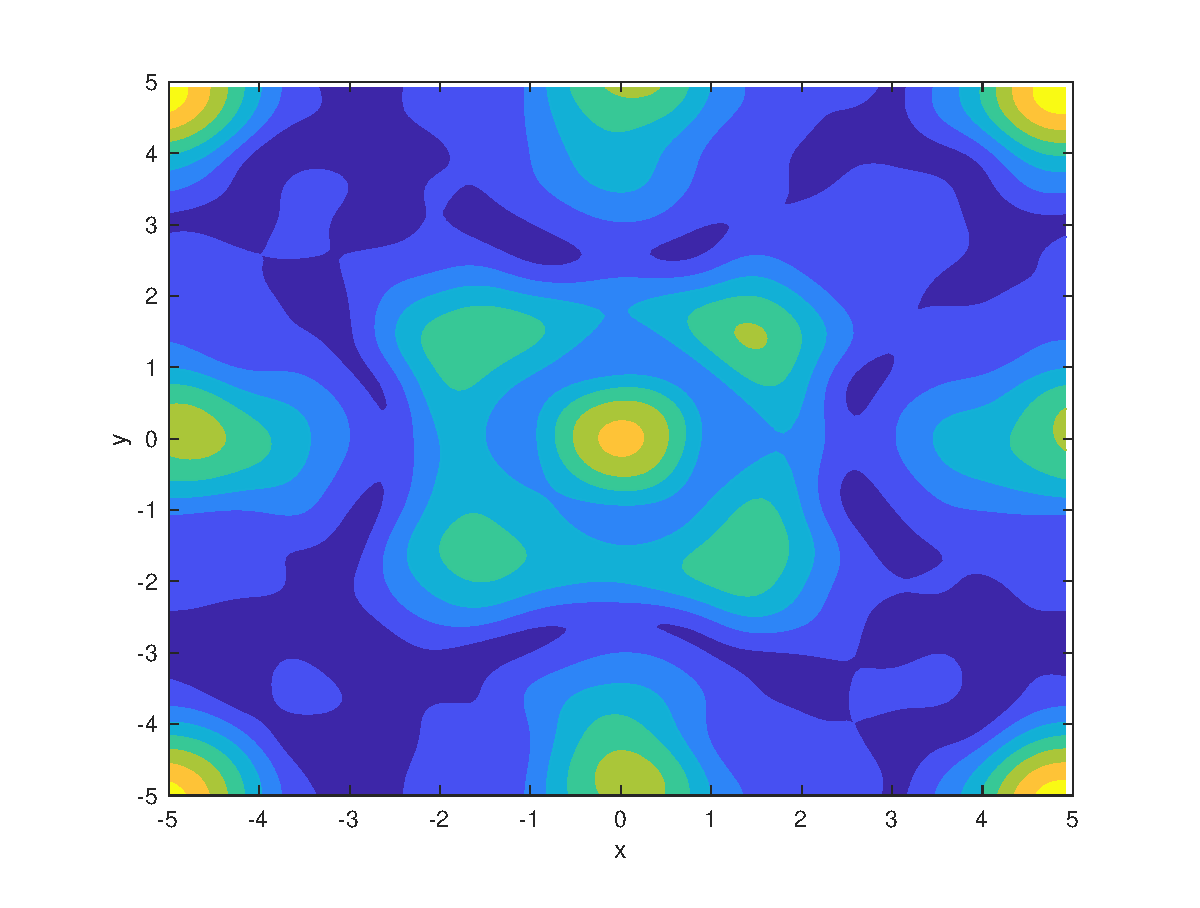
\includegraphics[width=0.3\textwidth]{./figure/exp2_contour3_p100.eps}
	}
	\caption{当$\alpha=1.3$ 时, 算例 \ref{exp_PAVF:4}的波传播图.}
	% \caption{The pictures of wave propagation for Example \ref{exp_PAVF:4} with $\alpha=1.3.$}
	\label{fig_PAVF:13}
	\end{center}
	\end{figure}

	\begin{figure}[H]
		\begin{center}
		 \subfigure[$t=0s$]{ \centering
		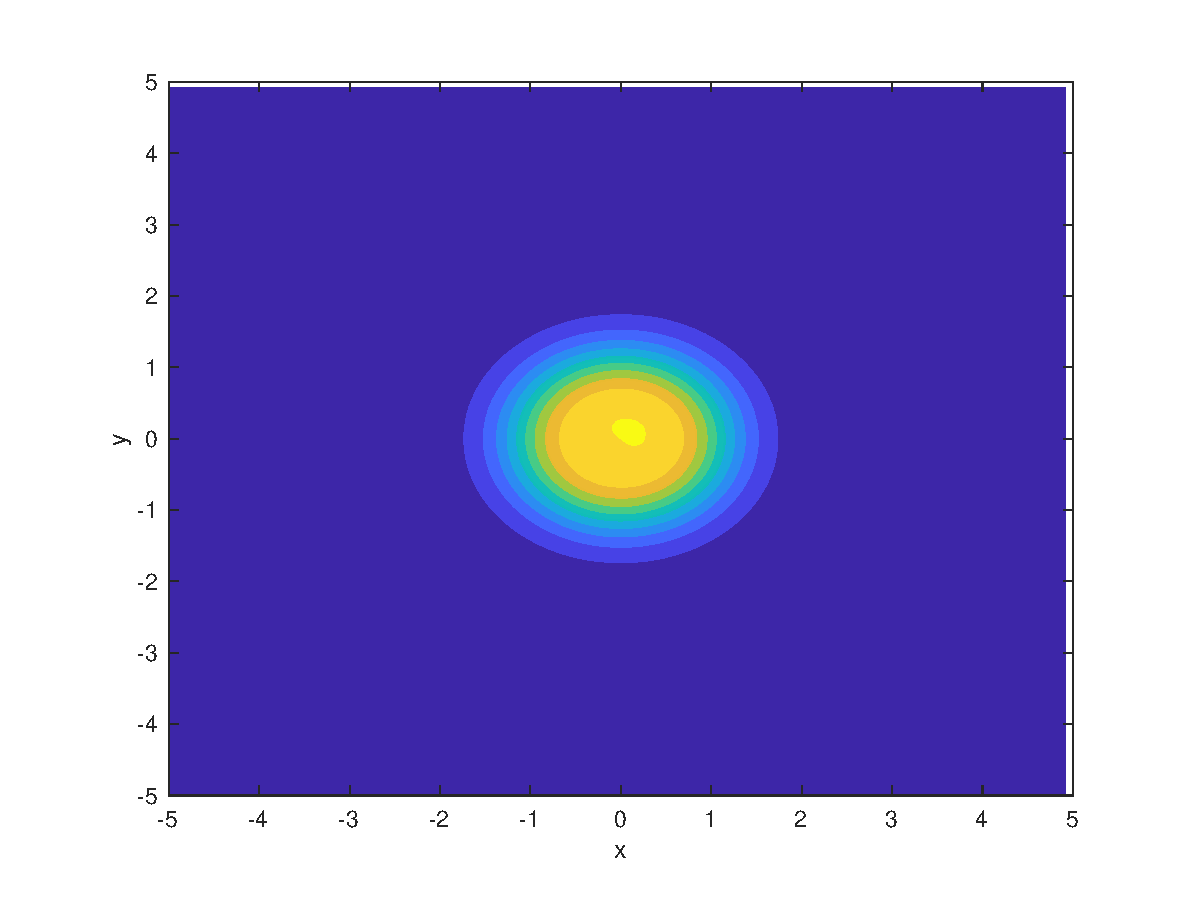
\includegraphics[width=0.3\textwidth]{./figure/exp2_contour6_p0.eps}
		}\subfigure[$t=1s$]{ \centering
		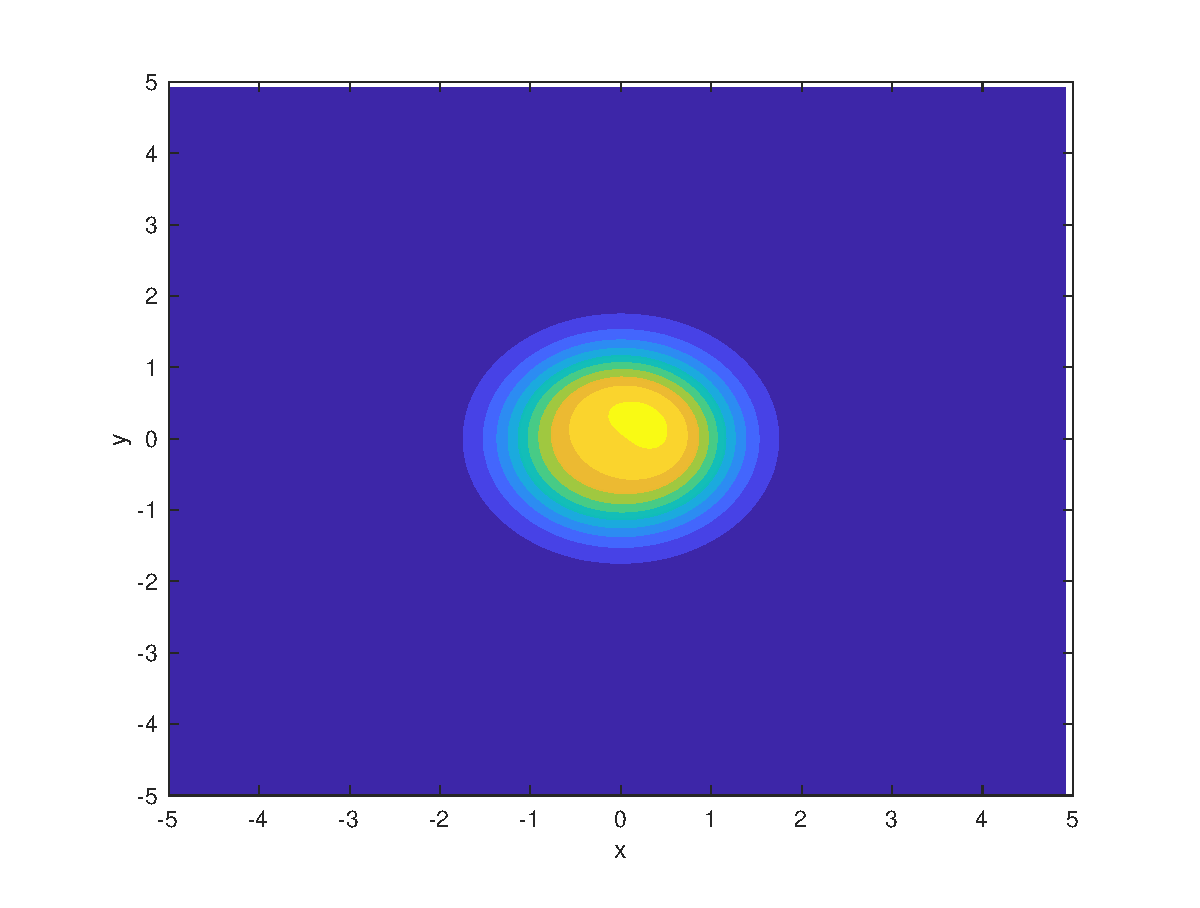
\includegraphics[width=0.3\textwidth]{./figure/exp2_contour6_p1.eps}
		} \subfigure[$t=5s$]{ \centering
		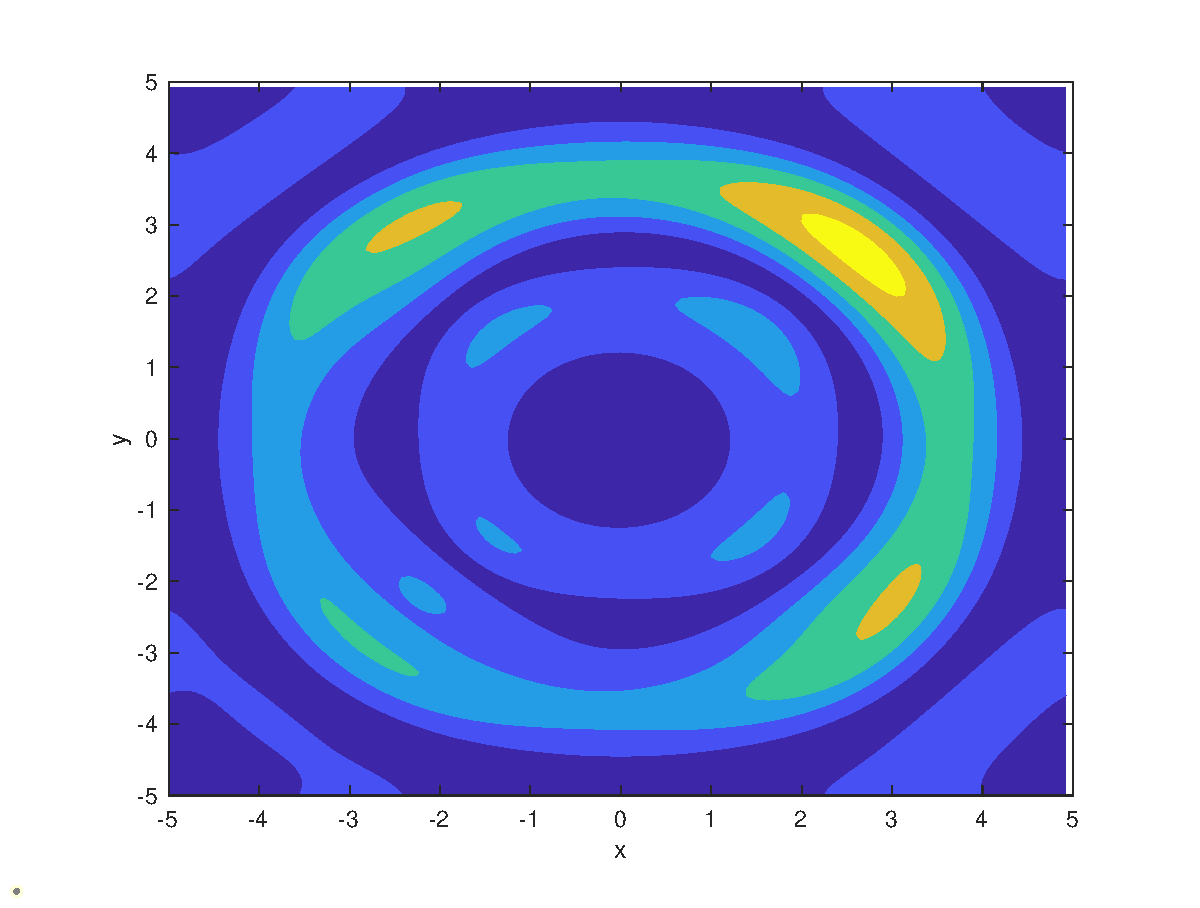
\includegraphics[width=0.3\textwidth]{./figure/exp2_contour6_p5.eps}
		}\\
		\subfigure[$t=10s$]{ \centering
		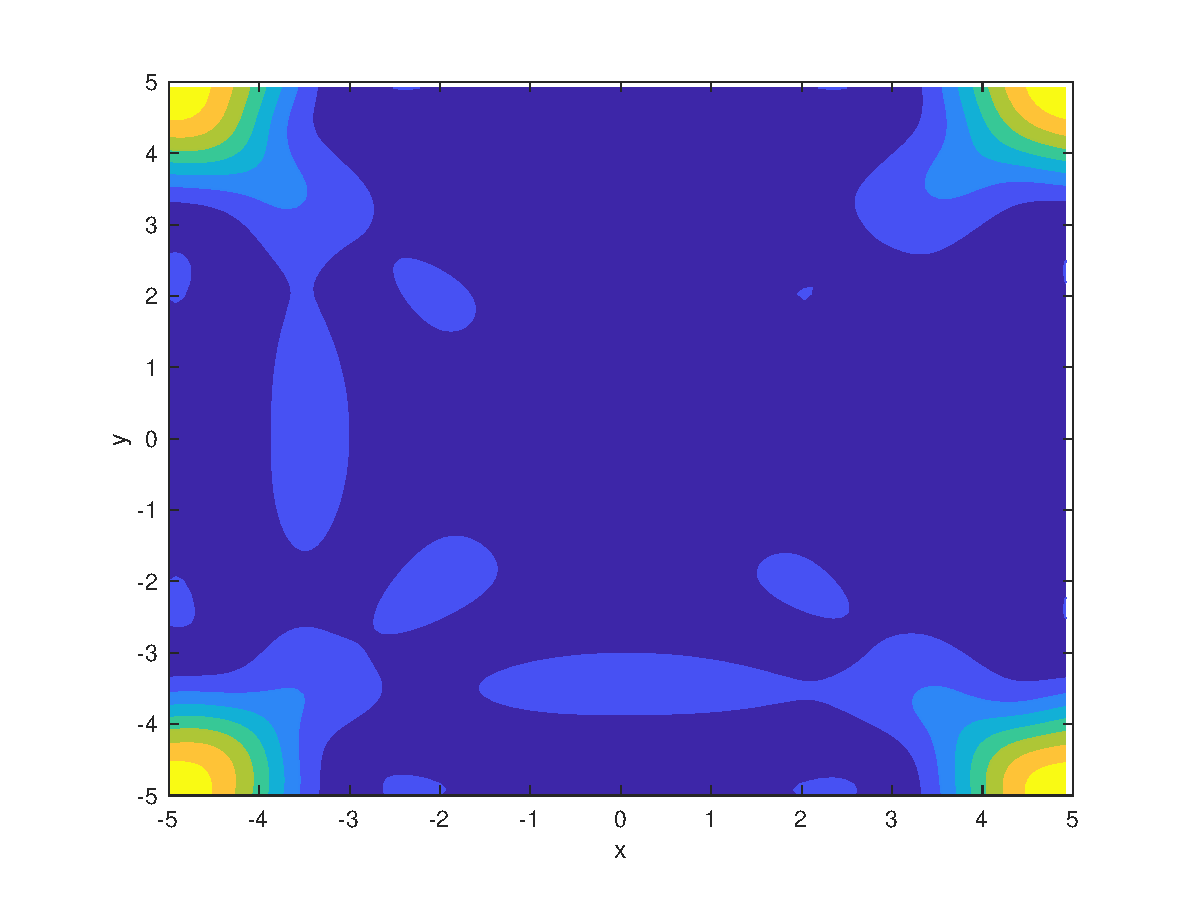
\includegraphics[width=0.3\textwidth]{./figure/exp2_contour6_p10.eps}
		}\subfigure[$t=50s$]{ \centering
		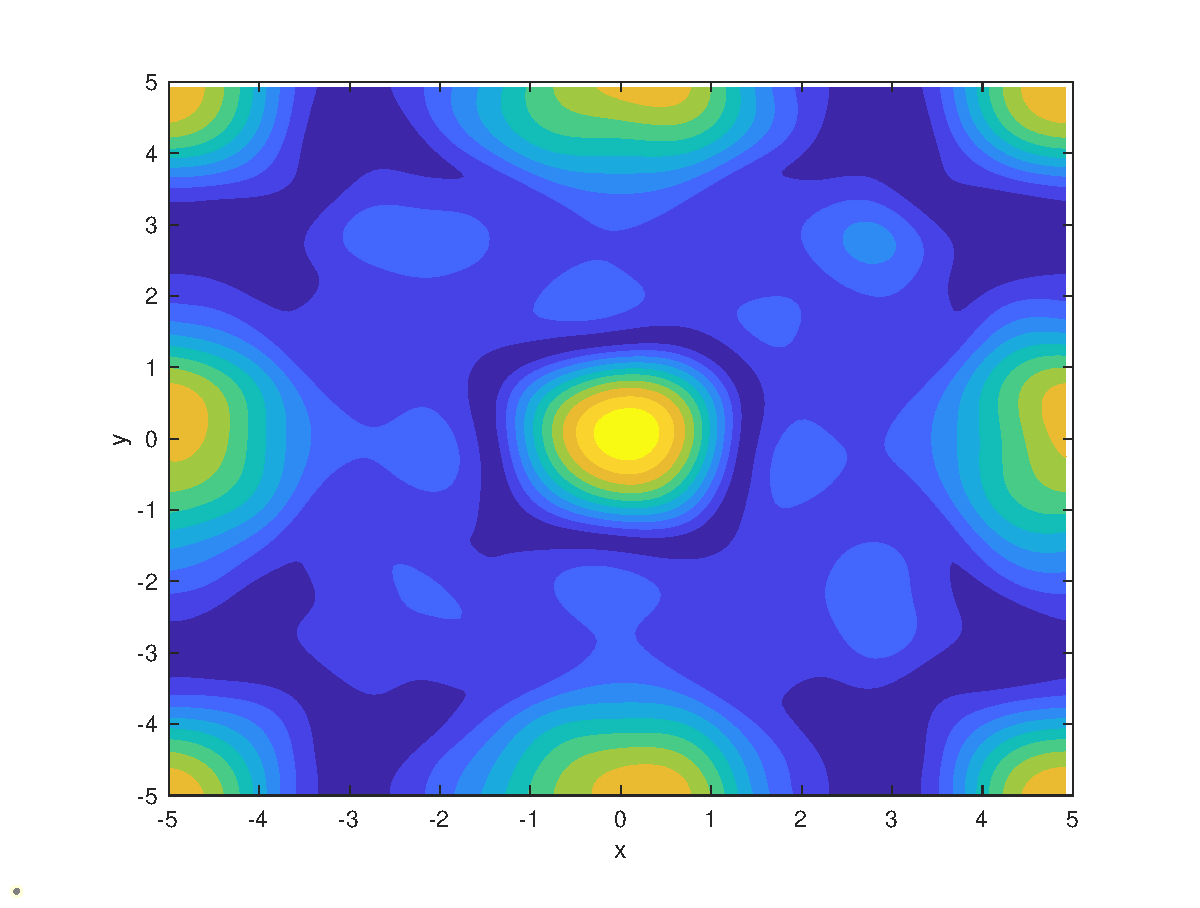
\includegraphics[width=0.3\textwidth]{./figure/exp2_contour6_p50.eps}
		} \subfigure[$t=100s$]{ \centering
		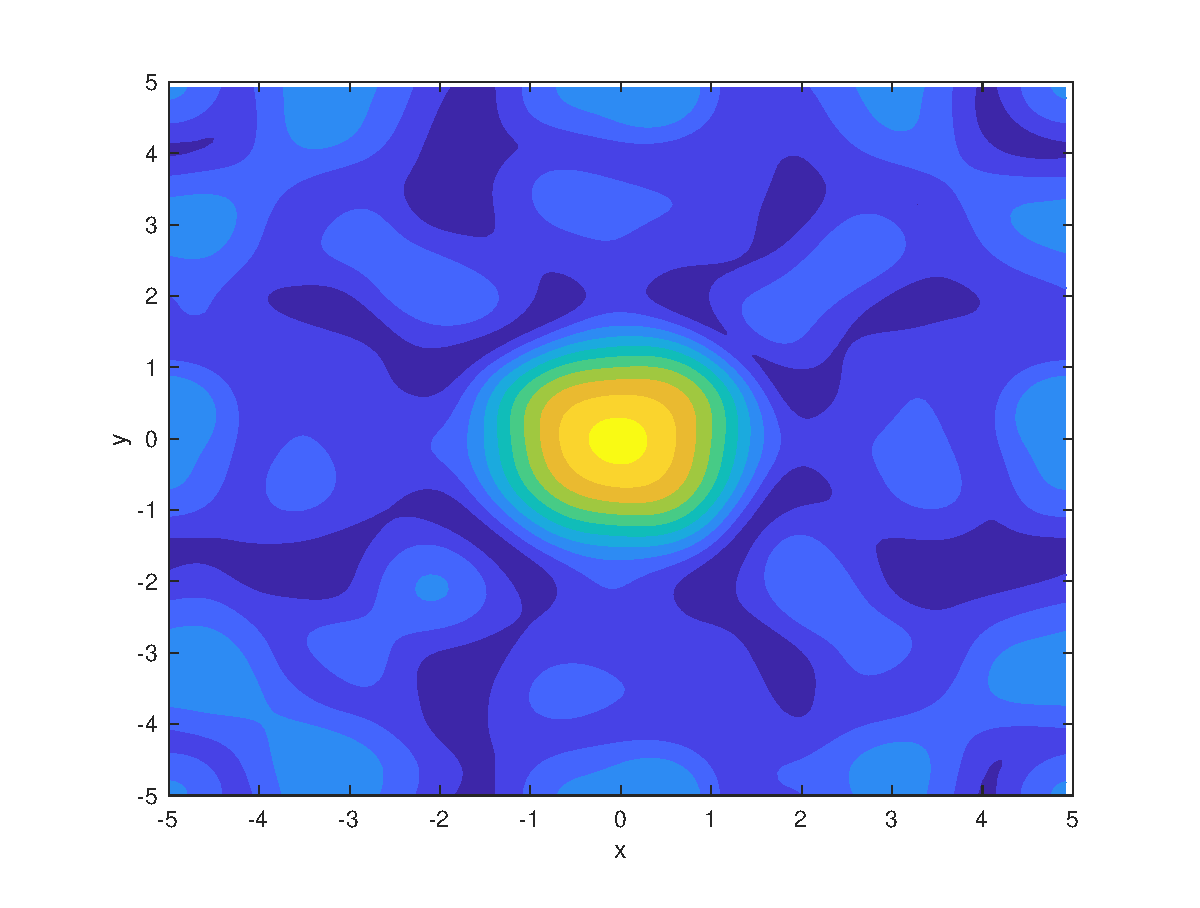
\includegraphics[width=0.3\textwidth]{./figure/exp2_contour6_p100.eps}
		}
		% \caption{The pictures of wave propagation for Example \ref{exp_PAVF:4} with $\alpha=1.6.$}
		\caption{ 当$\alpha=1.6$ 时, 算例 \ref{exp_PAVF:4}的波传播图.}
		\label{fig_PAVF:14}
		\end{center}
		\end{figure}

		\begin{figure}[H]
			\begin{center}
			 \subfigure[$t=0s$]{ \centering
			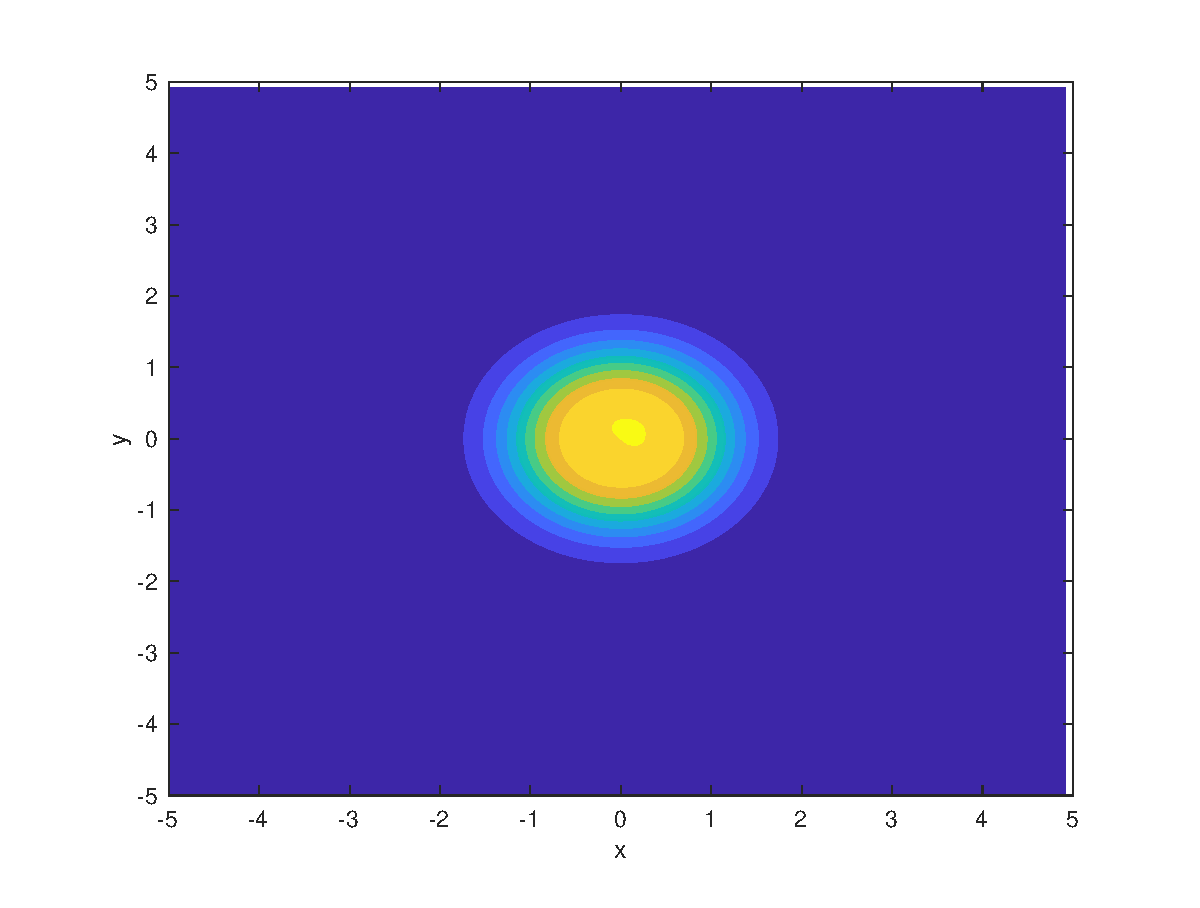
\includegraphics[width=0.3\textwidth]{./figure/exp2_contour99_p0.eps}
			}\subfigure[$t=1s$]{ \centering
			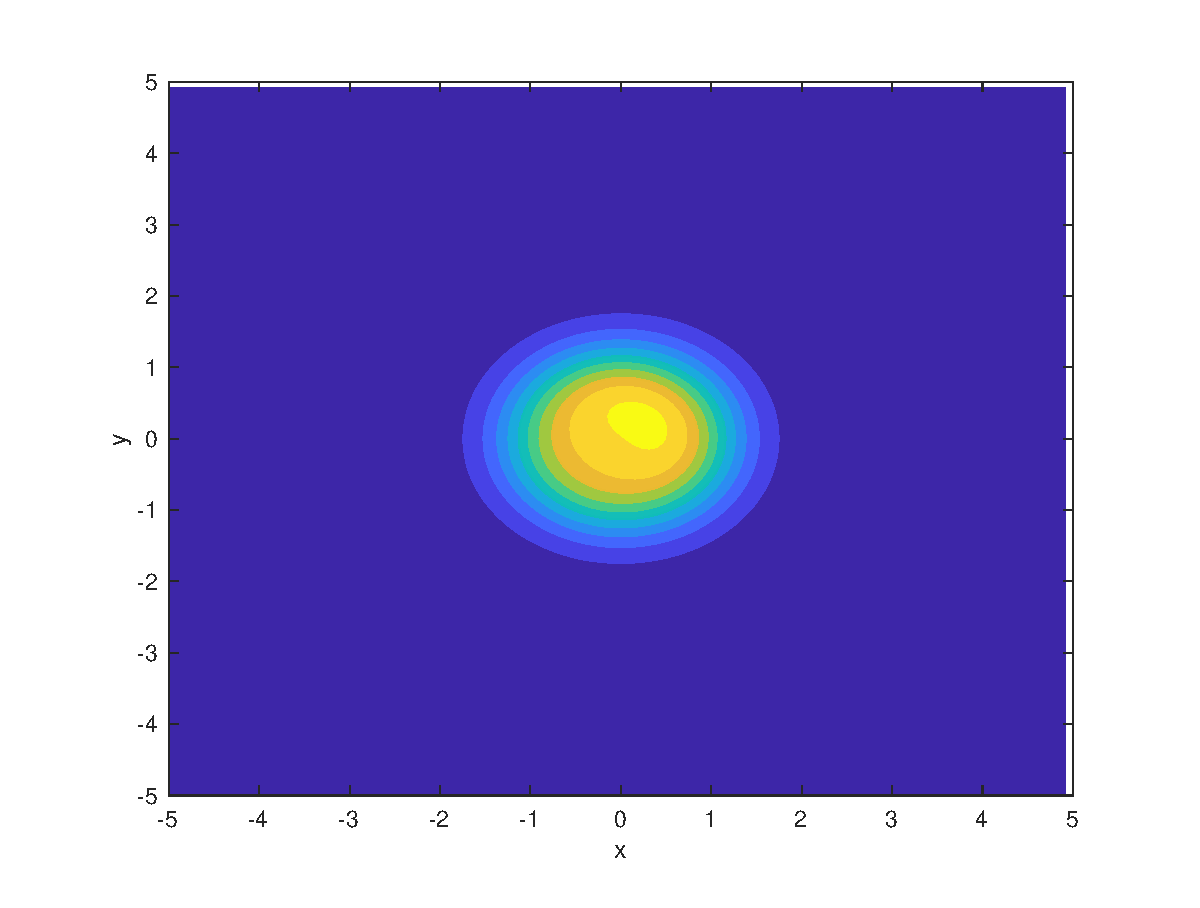
\includegraphics[width=0.3\textwidth]{./figure/exp2_contour99_p1.eps}
			} \subfigure[$t=5s$]{ \centering
			\includegraphics[width=0.3\textwidth]{./figure/exp2_contour99_p5.eps}
			}\\
			\subfigure[$t=10s$]{ \centering
			\includegraphics[width=0.3\textwidth]{./figure/exp2_contour99_p10.eps}
			}\subfigure[$t=50s$]{ \centering
			\includegraphics[width=0.3\textwidth]{./figure/exp2_contour99_p50.eps}
			} \subfigure[$t=100s$]{ \centering
			\includegraphics[width=0.3\textwidth]{./figure/exp2_contour99_p100.eps}
			}
			% \caption{The pictures of wave propagation for Example \ref{exp_PAVF:4} with $\alpha=1.99.$}
			\caption{当$\alpha=1.99$ 时, 算例 \ref{exp_PAVF:4}的波传播图.}
			\label{fig_PAVF:15}
			\end{center}
			\end{figure}
		
		%---------------------------------------------------------------------------------------------------------------------------
		\begin{figure}[H]
			\begin{center}
			 \subfigure[$t=0s$]{ \centering
			\includegraphics[width=0.3\textwidth]{./figure/exp2_contour2_p0.eps}
			}\subfigure[$t=1s$]{ \centering
			\includegraphics[width=0.3\textwidth]{./figure/exp2_contour2_p1.eps}
			} \subfigure[$t=5s$]{ \centering
			\includegraphics[width=0.3\textwidth]{./figure/exp2_contour2_p5.eps}
			}\\
			\subfigure[$t=10s$]{ \centering
			\includegraphics[width=0.3\textwidth]{./figure/exp2_contour2_p10.eps}
			}\subfigure[$t=50s$]{ \centering
			\includegraphics[width=0.3\textwidth]{./figure/exp2_contour2_p50.eps}
			} \subfigure[$t=100s$]{ \centering
			\includegraphics[width=0.3\textwidth]{./figure/exp2_contour2_p100.eps}
			}
			% \caption{The pictures of wave propagation for Example \ref{exp_PAVF:4} with $\alpha=2.$}
			\caption{当$\alpha=2.0$ 时, 算例 \ref{exp_PAVF:4}的波传播图.}
			\label{fig_PAVF:16}
			\end{center}
			\end{figure}

\section{小结}\label{Section_PAVF: 5}

在本章中,首先推导出了非线性分数阶薛定谔波动方程的哈密顿系统,基于等价的哈密顿系统,通过将分区平均向量场加方法与傅里叶拟谱方法结合构建了一个保结构数值格式.
理论分析和数值结果表明,所提出的方法能够有效地同时保持原始能量和质量.
